\documentclass[12pt]{article}

\usepackage{graphicx}
\usepackage{url}
\usepackage{chapterbib}
\usepackage[utf8]{inputenc}
\usepackage[english]{babel}
\usepackage[T1]{fontenc}
\usepackage{amsfonts}
\usepackage{xfrac}
\usepackage{amsmath,amssymb,amsthm}
\usepackage{fancyhdr}
\usepackage{multirow,array}
\usepackage{bbm}
\usepackage{hyperref}
% \usepackage[a4paper, margin=2.2cm]{geometry}
% \usepackage{geometry}[6.5,8]
\usepackage{float}
\usepackage{graphicx}
\graphicspath{ {./images/} }
\newcommand{\indep}{\perp \!\!\! \perp}
\usepackage{graphicx}
\usepackage{blindtext}
\newcommand{\mysection}[2]{\setcounter{section}{#1}\addtocounter{section}{-1}\section{Lecture #1: #2}}
\setcounter{tocdepth}{3}
\restylefloat{table}
\hypersetup{
    colorlinks = true,
    linkcolor = {blue}
}
\usepackage[authoryear,round]{natbib}
\bibliographystyle{plainnat}
\usepackage{pgfplots}
\pgfplotsset{compat=1.16}
\usepackage{tikz}
\usetikzlibrary{arrows.meta,positioning,calc}
\usepackage{caption}
\floatstyle{plaintop}
\restylefloat{table}
\usepackage{stackengine}
\usepackage{booktabs}
\usepackage{bbm}
\usepackage{multicol}
\newcommand{\blind}{0}
\usepackage{float,booktabs,tabularx,array,ragged2e}
\newcolumntype{Y}{>{\RaggedRight\arraybackslash}X}
\captionsetup[table]{position=top}
\usepackage{booktabs}
\usepackage{threeparttable}
\newcommand{\sym}[1]{\ifmmode^{#1}\else\(^{#1}\)\fi}
\usepackage{xcolor}

% ======================================================================
% notation_macros.tex — shared notation for the model & estimation sections
% Informality and financial frictions (Morales & Puggioni)
% \input this file once in the preamble of the main document.
% All definitions are guarded so they do not clash with an existing preamble.
% ======================================================================
 
% ---- theorem environments (guarded: skipped if already defined) ------
\makeatletter
\@ifundefined{proposition}{%
  \newtheorem{proposition}{Proposition}[section]
  \newtheorem{lemma}[proposition]{Lemma}
  \newtheorem{corollary}[proposition]{Corollary}
  \newtheorem{assumption}{Assumption}
  \newtheorem{remark}[proposition]{Remark}
  \newtheorem{definition}[proposition]{Definition}
}{}
\makeatother
 
% ---- generic math operators ------------------------------------------
\providecommand{\E}{\mathbb{E}}
\providecommand{\Prob}{\mathbb{P}}
\providecommand{\R}{\mathbb{R}}
\providecommand{\ind}[1]{\mathbf{1}\{#1\}}
\providecommand{\sgn}{\operatorname{sgn}}
\providecommand{\diff}{\mathrm{d}}
 
% ---- sectors and states ----------------------------------------------
% s \in {i,f}: informal (i), formal (f); "o" = out of the market (inactive)
\providecommand{\infml}{i}
\providecommand{\fml}{f}
\providecommand{\out}{o}
 
% ---- technology and prices -------------------------------------------
% y = theta k^alpha l^nu ; gamma = alpha/(1-nu) is the profit curvature in k
\providecommand{\curv}{\gamma}                    % gamma = alpha/(1-nu)
\providecommand{\prodx}{x}                        % x = theta^{1/(1-nu)}
\providecommand{\prodxhat}{\hat{x}}               % expected profitability index
\providecommand{\wgs}[1]{w_{#1}}                  % effective wage in sector s
 
% ---- profit primitives -----------------------------------------------
\providecommand{\Om}[1]{\Omega_{#1}}              % sector profit shifter
\providecommand{\prof}[1]{\pi_{#1}}               % static profit function
 
% ---- financial parameters --------------------------------------------
\providecommand{\spread}[1]{\phi_{#1}}            % toy model: linear spread phi_s
\providecommand{\spreadlev}[1]{\varsigma_{#1}}    % general: level of the spread
\providecommand{\spreadslope}[1]{\phi_{1#1}}      % general: slope of the spread
\providecommand{\spreadfix}[1]{\phi_{0#1}}        % general: fixed cost of borrowing
\providecommand{\collat}[1]{b_{#1}}               % collateral pledgeability b_s
\providecommand{\Fin}[1]{\Phi_{#1}}               % total financing cost function
 
% ---- user costs -------------------------------------------------------
\providecommand{\Rint}{R^{0}}                     % internal-funds user cost
\providecommand{\Rext}[1]{R_{#1}}                 % external user cost, sector s
 
% ---- costs, taxes, death ---------------------------------------------
\providecommand{\fc}[1]{c_{#1}}                   % per-period fixed cost c_s
\providecommand{\ec}[1]{c^{e}_{#1}}               % entry cost c^e_s
\providecommand{\swc}[1]{c_{#1}}                  % switching costs c_{if}, c_{fi}
\providecommand{\taxy}{\tau_{y}}                  % corporate / output tax
\providecommand{\taxl}{\tau_{\ell}}               % payroll tax
\providecommand{\death}[1]{\lambda_{#1}}          % exogenous death rate
\providecommand{\lwedge}[1]{\eta_{#1}}            % labor-wedge scale (audit cost)
 
% ---- productivity process --------------------------------------------
\providecommand{\pers}[1]{\rho_{#1}}              % AR(1) persistence, sector s
\providecommand{\sdi}[1]{\sigma_{\varepsilon #1}} % innovation s.d., sector s
\providecommand{\sdv}{\sigma_{v}}                 % permanent-component s.d.
\providecommand{\muko}{\mu_{k_0}}                 % entrant wealth: log-mean
\providecommand{\sdko}{\sigma_{k_0}}              % entrant wealth: log-s.d.
 
% ---- value functions and thresholds ----------------------------------
\providecommand{\Uv}[1]{U_{#1}}                   % continuation value by sector
\providecommand{\Vv}[1]{V_{#1}}                   % recursive value by sector
\providecommand{\thF}[1]{\hat{x}^{\mathrm{F}}_{#1}}   % formality threshold
\providecommand{\thX}[1]{\hat{x}^{\mathrm{X}}_{#1}}   % exit threshold
\providecommand{\thE}[1]{\hat{x}^{\mathrm{E}}_{#1}}   % entry threshold
\providecommand{\netw}{n}                         % internal funds at investment stage
\providecommand{\Kop}[1]{\mathcal{K}_{#1}}        % K_s = beta(1-lambda_s)c_s
\providecommand{\Xth}[1]{\mathcal{X}_{#1}}        % master exit/entry threshold


\addtolength{\oddsidemargin}{-.5in}
\addtolength{\evensidemargin}{-1in}
\addtolength{\textwidth}{1in}
\addtolength{\textheight}{1.7in}
\addtolength{\topmargin}{-1in}


\begin{document}


\def\spacingset#1{\renewcommand{\baselinestretch}
{#1}\small\normalsize} \spacingset{1}


%%%%%%%%%%%%%%%%%%%%%%%%%%%%%%%%%%%%%%%%%%%%%%%%%%%%%%%%%%%%

\if0\blind
{
    \title{\bf Formality as a Financing Decision}
  \author{David Morales \thanks{Toulouse School of economics, david.morales@tse-fr} \quad Daniela Puggioni \thanks{Banco de México, dpuggionih@banxico.org.mx}}
  \date{October 2026 \\
  \vspace{3mm}
  \textcolor{lightgray}{Work in Progress. Latest version available
    \href{https://davidsmorales.github.io/files/FinancialFrictions.pdf}{here}%
  }%
}
\maketitle
} \fi

\if1\blind
{
  \bigskip
  \bigskip
  \bigskip
  \begin{center}
    {\LARGE\bf Title}
\end{center}
  \medskip
} \fi

\bigskip

\begin{abstract}
Can bank loans affect the formality decision of informal firms? We match the universe of bank loans, the social security records, and the economic censuses in Mexico to observe formality, loans, and firm transitions. Three facts emerge: three quarters of firms with a bank loan are informal; informal firms pay higher rates, post more collateral and obtain smaller loans; and firms move between formality and informality, both directions. In a dynamic model, firms that need a loan and are near to indifference between formal and informal change their status when the relative terms or availability of loans change. Using leave-one-out shift-share bank credit supply shocks, we find that a ten percent credit supply expansion raises the financial advantage of formal firms and, consequently, increases formalization by 0.5 percent and decreases formal-to-informal transitions by 0.4 percent. Our contribution is to show that bank loans affect informal firms as well as formal ones, and with them the share of formal firms.
% The effects of the financial sector on formal firms are well known in the literature. However, little is known about its effects on the informal sector. This paper closes this gap by asking: Can bank loans affect the formality decision of firms, especially of those already in the informal sector? To answer it, we match the universe of bank loans, the administrative social security records, and the economic censuses in a dataset that contains formality, bank loans, and firm transitions on the same markets over twenty years. We document three stylized facts. First, informal firms are inside the banking system, in contrast to what is commonly assumed. Second, informal firms face worse loan terms than their formal counterparts. Third, firms move regularly between formality and informality, in both directions. The paper builds a dynamic model in which firms choose whether to be formal based on the trade-off between tax costs and financial benefits. The main argument is that firms close to indifference between being formal or informal and in need of a loan reverse their formality status after a relative change in the terms or availability of loans. The empirical strategy uses a Shift-Share design to confirms the model prediction and shows that a credit supply shock raises the financial advantage of formal firms and, consequentially, increases formalization and decreases formal-to-informal transitions. The results imply that policies that affect the relative loan advantage of formal firms, from credit guarantees to bank competition, can shift the share of formal firms. 
\end{abstract}

\noindent\textbf{Keywords:} informality, firm dynamics, financial frictions, credit supply, formalization.
\vfill

\newpage
\spacingset{1.2} 

\section{Introduction}
\label{1}

The effects of the financial sector on formal firms are well known in the literature. However, little is known about its effect on the informal sector. The reason is that there is little data on informality and the financial sector. This paper overcomes this data limitation, uncovers stylized facts linking informality and finance, and addresses the following research question: Can bank loans affect the formality decision of firms, especially of those already in the informal sector? We show that credit supply expansions reach informal firms but improvement in terms and volume is higher for formal ones. This differentiated effect increases the financial advantage of formal firms and changes the two-way formality transitions. A ten percent expansion raises formalization by 0.5 percent and lowers informalization by 0.4 percent.

This paper matches the universe of bank loans to social security administrative records at the firm level to uncover the formality of borrowers, the loan position of formal firms, and the difference in loan terms between formal and informal enterprises. It contains nearly  3.3 million firms, 1.3 million borrowing and 2.2 million formal, across 119 banks between 2005 and 2025 (Appendix~\ref{app:data}). However, informal firms without a bank loan escape this dataset. To overcome this problem, we merge these two datasets to the economic censuses, which is only possible at the market level, to observe all types of firms over time: formal and informal, borrowers and non-borrowers. The resulting dataset is unique because it contains formality, bank loans, and firm transitions on the same markets over twenty years. As a result, we can study a previously unexplored relationship: the effect of bank loans on informal firms. 

With these data, we document three stylized facts. First, informal firms are inside the banking system, in contrast to what is commonly assumed. Figure~\ref{fig:borrowing_shares} reveals that among all the firms holding a bank loan in Mexico, 74 percent are informal\footnote{An establishment is informal when it reports zero social security contributions in the census while earning income, the census classification used throughout the paper (Section~\ref{sec:data}).}. Therefore, informal firms are directly exposed to bank loan conditions. However, because the informal sector is so large, the share of informal firms with a bank loan represents only 5 percent, against 13 percent for formal firms.

\begin{figure}[H]
    \caption{Borrowing shares by formality}
    \label{fig:borrowing_shares}
    \centering
    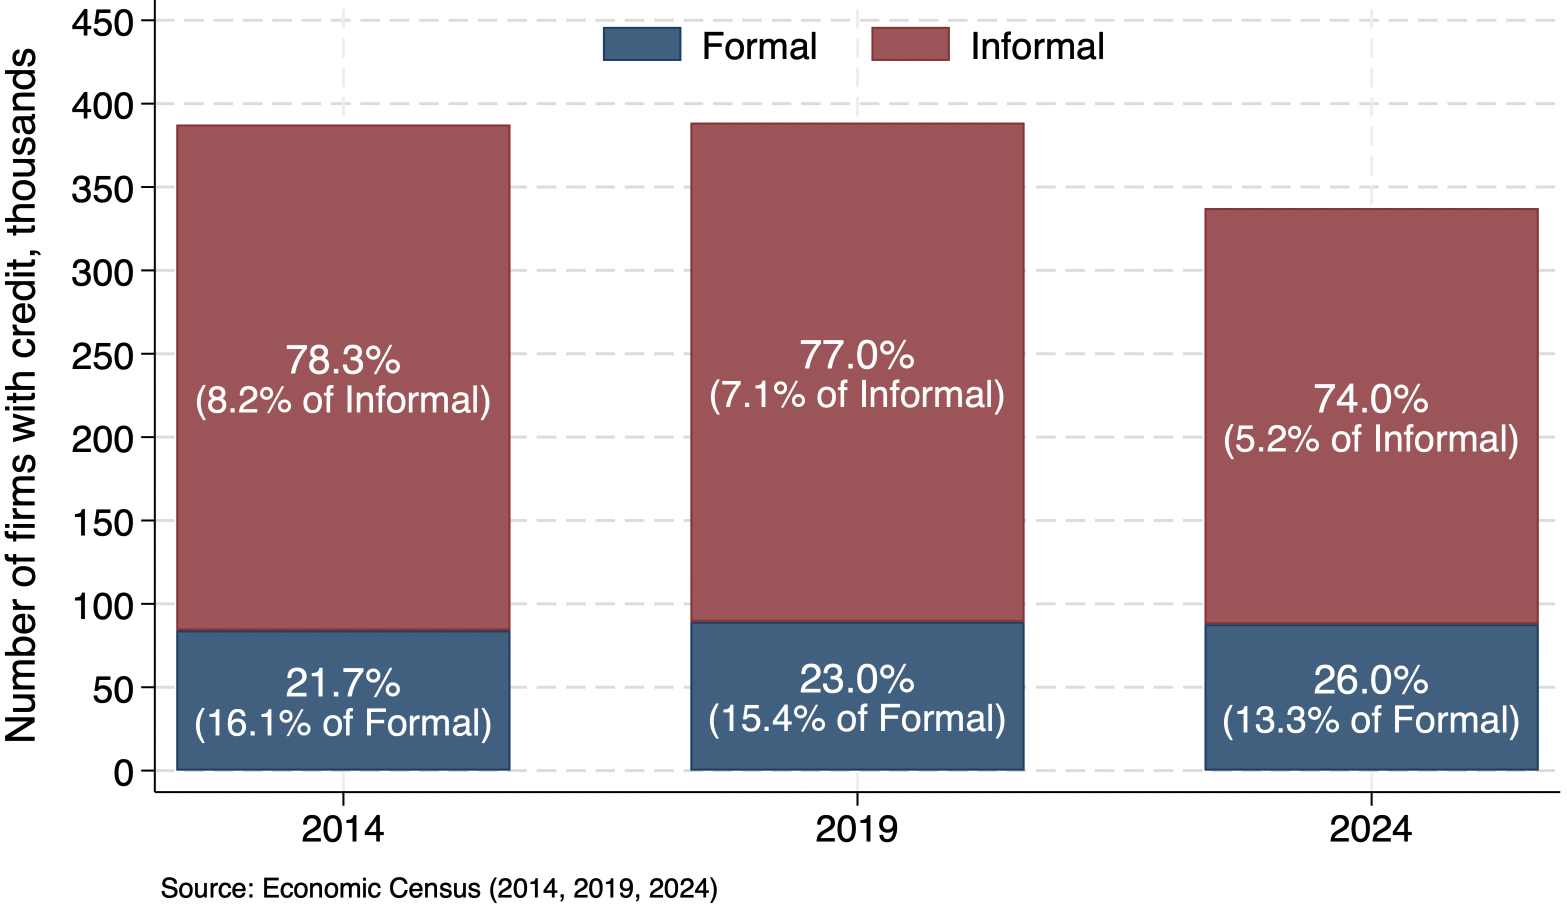
\includegraphics[scale=0.2]{slides_material/firm_dist_g.png}
\end{figure}

Second, informal firms face worse loan terms than their formal counterparts. Table~\ref{tab:desc_firms} demonstrates that, at the median, an informal firms pay an interest rate $0.7$ percentage points higher, need $3$ percentage points more collateral, and obtain $33.2$ thousand dollars smaller loans than a formal firm. These differences hold for the 10th and 90th percentiles\footnote{With the exception of collateral at the 90th percentile} and, in general, for the majority of the distribution. 

Third, formality status is not permanent and it can change, potentially due to changes in the economic environment, like the financial conditions. Table~\ref{firms_transition} shows that between 11.6 and 21.8 percent of formal firms become informal in five years, while between 3.5 and 6.5 percent of informal firms formalize. In contrast to previous work that treats formality as an absorbing state from which firms cannot transition into informality \citep{meghir2015wages, ulyssea2018firms}, we see formality transitions as two-way\footnote{The formal-to-informal and informal-to-formal transitions are not an artifact of the definition of informality. Appendix~\ref{transitions_alternative} documents that these transitions exist under alternative definitions of informality: accounting for the intensive margin (Table~\ref{transition_intensive}), using the social security number (Table~\ref{transition_imss}), or using the tax number (Table~\ref{transition_rfc}).}.

To understand the plausible mechanisms that link formality decisions to the financial sector, we build a parsimonious dynamic model in which firms choose each period between formality, informality, and exit. Formality carries taxes and higher operating costs but better financial terms (lower marginal loan cost and more pledgeable collateral) while informality saves the taxes and has lower operating costs but faces detection costs that grow with size and worse financial terms. Therefore, the formality decision trades off the tax cost with the financial benefits of being formal. The model predicts that a relative improvement in the terms or availability of loans for formal firms with respect to the informal ones, should increase formalization and decrease formal-to-informal transitions, for firms that need additional loans. 

The model predictions are tested in the empirical section, where the challenge to claim causality is endogeneity in the form of reverse causality (formality affecting financial conditions and not the inverse) and unobserved common characteristics (only productive firms formalize and hold a bank loan). To overcome this challenge we rely on a Leave-One-Out Shift-Share Instrumental Variable (LOO-SSIV) with exogenous shift. 

This method disentangles the changes in credit within firms that borrow from several banks into supply (bank fixed-effects) and demand (firm fixed-effects) \citep{khwaja2008tracing, amiti2018much}, leaving the market of interest outside of the estimation sample. Afterwards, it computes the predetermined bank shares in the market of interest. The final instrumental variable is the aggregation of the shift (bank fixed-effects), weighted by the share (bank market-shares), as in the quasi-experimental Shift-Share framework of \citet{borusyak2022quasi}.\footnote{Inference uses the exposure robust standard errors of \citet{adao2019shiftshare}. As a robustness, we report the wild cluster bootstrap probabilities \citep{cameron2008bootstrap}. The design rests on roughly seventeen effective bank shocks, no single bank carries more than 17 percent of the exposure weight, and the results survive rebuilding the instrument without the largest lender, at a cost in precision (Tables~\ref{shock_stats} and \ref{drop_top_bank_table}).} The instrument is strong, with a first stage $F$ statistic above $265$, and a one standard deviation shock roughly doubles five year market credit.

The model predictions are corroborated. Improving the formal advantage in loan terms and availability increases formalization and reduces formal-to-informal transitions. A credit supply expansion yields $25$ percent less collateral, $19$ percent more credit, and half a percentage point cheaper loans for formal firms four years after the shock; whereas for informal firms the volume response is smaller ($16$ percent), rates do not change ($-0.1$ percentage points, not significant), and collateral falls by less ($13$ percent). The credit supply shock amplifies the formal financial advantage and, in consequence, as predicted by the model, causally raises formalization by $0.5$ percent and lowers formal-to-informal transitions by $0.4$ percent, after a ten percent increase in credit. That is about  $850$ additional transitions from informal to formal and $600$ fewer in the opposite direction across the markets in our sample. The results imply that policies that affect the relative loan advantage of formal firms, from credit guarantees to bank competition, can shift the share of formal firms. These main results are robust to balance, pretrend and placebo tests, the removal of the largest lender and of the largest markets, and a shock-level design with re-identified shocks (Section~\ref{robustness}).

Additionally, for a ten percent increase in credit supply the stock of formal firms rises by $0.5$ percent, the formal entry rises by $0.7$ percent, and exit rises by $0.5$ percent, mostly among informal firms. Regarding the number of firms holding a loan, it increases $0.4$ percent among formal and $0.3$ percent among informal firms. Thus, the shock changes the terms and size of the loan, not who can borrow. On the real side, and less precisely estimated, the formal wage bill rises by $0.2$ percent and the formal employment by $0.2$ percent, whereas the mean wage falls marginally. The value added falls by $0.5$ percent in the informal sector and does not move in the formal one.

The paper's contribution lies in showing that bank loans also affect informal firms, and not only the formal ones, and that this effect has broader implications on formality shares, the labor market, and average productivity. Moreover, we contribute to three literatures, developed in Section~\ref{2}. To the credit supply literature it adds the margin that previous work could not incorporate: informality. To the informality literature it adds a financial lever that moves the formality margin. To the literature on firm dynamics with financial frictions it adds quasi-experimental evidence on how financing terms shape the formality choice in a firm dynamics setting. The main limitation of this work is the absence of general equilibrium effects and competition in the loan, labor, and goods markets. More research is needed to address these limitations and to better understand the effects of the financial sector on informality.

The paper proceeds as follows. Section~\ref{2} reviews the literature. Section~\ref{sec:data} describes the data and Section~\ref{sec:descriptives} the descriptive stylized facts. Section~\ref{sec:toy} builds the dynamic model, Section~\ref{empirical_strategy_section} develops the identification strategy,  and Section~\ref{results} presents the results. Section~\ref{conclusion} concludes.

\section{Literature review} \label{2}

This paper speaks to three literatures. The first traces credit supply shocks to real outcomes. A within firm identification strategy introduced by \citet{khwaja2008tracing} separates bank supply from firm demand using multibank borrowers, \citet{amiti2018much} extend it to granular bank shocks, and \citet{degryse2019identifying} recover shocks from market and sector cells so that single bank firms contribute as well. On the real side, \citet{chodorow2014employment} shows that firms attached to distressed banks cut employment in the United States, \citet{greenstone2020credit} find small aggregate effects of local lending shocks in normal times, and \citet{gutierrez2023credit} show that in Mexico a one standard deviation credit supply shock raises formal employment growth by about 1.4 percentage points.\footnote{The response is not confined to marginal borrowers. \citet{melcangi2024precautionary} shows that even unconstrained firms hoard cash and shed employment in a credit crisis.} These designs share a constraint. Credit registries and social security records observe the formal sector by construction, so the outcome margin stops at the boundary of formality. By matching the universe of business loans to an economic census that counts informal establishments, we move the outcomes past that boundary and find that credit supply operates on the boundary itself. Credit expansions leave the total number of firms unchanged and recompose it instead, with more formal firms, faster formalization, and slower movement back to informality.\footnote{The instrument follows the quasi-experimental Shift-Share framework of \citet{borusyak2022quasi}, with exposure robust inference from \citet{adao2019shiftshare} and diagnostics in the spirit of \citet{goldsmith2020bartik}.}

The second literature studies informality and the policies that move it. The modern reading treats informal firms as a margin of development rather than a tax dodge alone, with \citet{la2014informality} and \citet{busso2012formal} documenting their prevalence and productivity costs, \citet{ulyssea2018firms} modeling the choice between registering the firm and hiding workers in Brazil, and \citet{meghir2015wages} embedding the sector choice in labor market search. The policy levers this literature evaluates are fiscal and administrative. Tax simplification in Brazil raised formality modestly \citep{rocha2018lower}, enforcement raises it at a cost \citep{almeida2012enforcement}, and the Mexican quasi-experimental record on tax side reforms finds formality responses near zero \citep{campos2020effects,bobba2021labor}.\footnote{Field experiments that subsidize registration find similarly small and often transitory effects, as in the Nicaraguan intervention studied by \citet{sutter2017transitioning}.} Relative to this work, the lever here is financial rather than fiscal, and the evidence is causal at the market level, so the paper documents that credit terms move the formalization margin that enacted tax reforms in the same country did not. The model matches this evidence in kind. Formality is a firm level status with entry, exit, and switching in both directions, disciplined by census transition rates, rather than an absorbing state.\footnote{\citet{adom2025structural} estimates a related transition model for Nigeria. The financial side here is richer, with participation costs, spreads, and collateral capacities by sector, and it is identified from quasi-experimental variation rather than from the cross section alone.}

The third literature puts financial frictions into firm dynamics. The tradition runs from \citet{hopenhayn1992entry} through \citet{cooley2001financial} and \citet{gomes2001financing}, with borrowing limits founded on limited enforcement in \citet{albuquerque2004optimal} and \citet{clementi2006theory}, development applications in \citet{arellano2012firm}, \citet{midrigan2014finance}, and \citet{moll2014productivity}, and wealth constrained entry going back to \citet{evans1989estimated}. Closest to this paper, \citet{d2012financial} and \citet{erosa2023public} study informality in economies with financial frictions, where the sector choice responds to financing conditions.\footnote{\citet{erosa2023public} model both the intensive and the extensive margins of evasion. Here the intensive margin is deliberately shut down so that the model's sector indicator matches the census classification behind every empirical moment.} we contribute on two fronts. The estimation disciplines the financial block with quasi-experimental moments, stacking the Shift-Share coefficients with the census cross section, so the incidence of an actual credit supply shock is an estimated object rather than a calibrated one. And the estimates locate the binding friction in a place this literature rarely prices, the fixed cost of participating in formal finance, which at twenty six wage units dwarfs the spread and collateral gaps. The three strands meet in one sentence. Formality is also a financing decision.

\section{Data}
\label{sec:data}

This work uses three microdata sources and the Bank of Mexico definition of local labor markets in Mexico. The first data source is the credit registry and includes the universe of bank loans to formal and informal firms, where amounts, costs, and collateral requirements are observed. The second source are the social security records that measure formal employment and wages. The third dataset is the economic census, which is a quinquennial survey of formal and informal establishments, on which we can follow establishments over time. 

The credit registry is generated by the banking commission (CNBV) from the regulatory report R04C that every bank has to file by law.\footnote{There is an aggregate, public version of this data available on the commission's website. We used the individual non-public version, accessed through the Bank of Mexico secured environment, EconLab, where all the information is anonymized.} This data includes the universe of commercial bank loans to businesses, from 2005 to date, at a monthly frequency. The characteristics of each loan are included, such as the amount, the interest rate, the collateral requirement, and the anonymized identity of the firm. It includes 119 banks and 1.3 million borrowing firms, between 2005 and 2025.

The social security records (IMSS) cover the universe of registered employers and their workers, formal by definition. Wages are daily base salaries, which include cash payments, bonuses, commissions, and payments in kind.\footnote{Wages are bottom coded at the minimum wage and top coded at twenty five times the Mexico City reference minimum. The unit of observation is a job rather than a person, so a worker holding two registered jobs contributes twice to our employment counts.}

The economic census (INEGI) surveys establishments with fixed physical facilities every five years, and the analysis uses the 2009, 2014, 2019, and 2024 waves.\footnote{The census is representative of localities with more than 2{,}500 inhabitants and non-agricultural sectors. Activity without a fixed physical facilities, like street vending, are excluded.} An establishment in the economic census is informal if it reports positive income and workers but zero social security contributions, formal otherwise. The economic census allows us to identify entry, exit and formality transitions of establishments, as well as their value added.

The 777 Local Labor Markets (llm) in the country are constructed by the Bank of Mexico using commuting flows\footnote{The methodology and information is published in the \href{https://www.banxico.org.mx/DataSetsWeb/dataset?ruta=LLM&idioma=en}{Bank of Mexico's market analysis}.}. Credit is observed in 705 of them, and the estimation sample of the main specification in Section~\ref{empirical_strategy_section} keeps the 556 markets in which the instrument covers at least half of baseline credit, which translates into 1{,}390 market-year observations across the census windows. 

To combine the datasets, first, we matched the credit registry and the social security records at the firm level. This match makes possible to identify the formality of the borrower, which is informal if it does not appears in the social security records, formal otherwise. The matched data contains 3.3 million firms. Notice that the credit-social security merged data includes formal firms with and without loans, and informal firms with loans; however, it does not capture informal firms that do not have a bank loan. To overcome this problem we merge the previous matched datasets to the economic census at the market level. By doing this we are able to identify all the formal and informal establishments, with or without loans, at a market level and follows them over time.\footnote{Figure~\ref{fig:inf_validation} in Appendix~\ref{transitions_alternative} compares the informality share of firms with bank loans from two different sources: the credit-social security matched registries and the economic census. The average level is similar, 76 percent against  81 percent in the census. However, at the state level the differences are higher, mainly due to the differences in the definition of establishment and firm.} 

The final dataset excludes agriculture, mining, construction, transport, financial services, and government. Borrowers whose main address is outside of the country are excluded. The monthly credit registry and social security records are made annual by keeping only the January snapshot. We keep only observations with valid locality and activity codes. All the merges are made using anonymized versions of the tax number (RFC), social security number (IMSS), and borrower ID. All the data construction and definitions are collected in Appendix~\ref{app:data}.

The combination of these three datasets allows us to observe credit, formality, and firm dynamics in the same markets over twenty years, something unique in a dataset. The effects of bank loans on informal firms is relatively unexplored, mainly due to the unavailability of the data. In contrast, the uniqueness of this data allows us to uncover the fact that bank loans reach the informal sector, and the conditions under which this happens, which is a central argument of this paper. 

\section{Descriptive statistics}
\label{sec:descriptives}

This section provides general descriptive statistics of the matched dataset. However three stylized facts stand out for their relevance and implications. The most important and poorly documented descriptive fact from the data is that informal firms are not outside the banking system, corroborated by two different sources. Table~\ref{tab:desc_firms} reveals that in 2024, between 67 (credit-social security registry) and 74 (census) percent of firms with bank loans were informal. This means that changes in credit conditions affect informal firms directly.

\begin{table}[H]
    \centering
    \caption{Descriptive statistics on firms, credit, and formality}
    \label{tab:desc_firms}
    \begin{threeparttable}
        \small
        \begin{tabular}{l r r r}
            \toprule
             & Formal & Informal & All \\
            \midrule
            \multicolumn{4}{l}{\textit{Panel A. Firms and bank credit: Economic Census 2024}} \\
            \addlinespace
            Firms & 658,065 & 4,810,115 & 5,468,180 \\
            Share of firms (percent) & 12.0 & 88.0 & 100.0 \\
            % Firms without a bank credit & 570,277 & 4,560,527 & 5,130,804 \\
            Firms with bank credit & 87,788 & 249,588 & 337,376 \\
            Credit incidence (percent of firms) & 13.3 & 5.2 & 6.2 \\
            Share of borrowers (percent) & 26.0 & 74.0 & 100.0 \\
            \addlinespace
            \multicolumn{4}{l}{\textit{Panel B. Credit terms by borrower status: credit registry, pooled 2005-2025}} \\
            \addlinespace
            Borrower years & 1,089,934 & 4,132,779 & 5,222,713 \\
            Borrowers, 2024 & 83,334 & 171,635 & 254,969 \\
            Unique borrowers, 2005--2025 & 210,895 & 1,114,533 & 1,269,287 \\
            Banks per borrower, mean & 1.35 & 1.14 & 1.19 \\
            Borrowers with two or more banks (percent) & 23.9 & 10.2 & 13.1 \\
            Credit records per borrower, mean & 4.32 & 2.32 & 2.74 \\
            \addlinespace
            \multicolumn{4}{l}{Authorized credit per borrower (thousand dollars)} \\
            \quad 10th percentile & 5.9 & 2.2 & 2.6 \\
            \quad Median & 47.9 & 14.7 & 17.2 \\
            \quad 90th percentile & 631.8 & 184.2 & 263.2 \\
            \addlinespace
            Interest rate (percent) & & & \\
            \quad 10th percentile & 9.3 & 10.0 & 9.9 \\
            \quad Median & 15.5 & 16.2 & 16.0 \\
            \quad 90th percentile & 24.4 & 29.0 & 28.0 \\
            \quad Mean & 16.1 & 18.5 & 17.9 \\
            \addlinespace
            Relationships without collateral (percent, 2010-2024) & 80.2 & 88.1 & 86.2 \\
            \multicolumn{4}{l}{Collateral to authorized credit, collateralized relationships} \\
            \quad 10th percentile & 0.05 & 0.06 & 0.05 \\
            \quad Median & 0.45 & 0.48 & 0.47 \\
            \quad 90th percentile & 1.45 & 1.31 & 1.36 \\
            \bottomrule
        \end{tabular}
        \begin{tablenotes}[flushleft]
            \item \footnotesize \textit{Notes:} Panel A source is the 2024 Economic Census, where informal is defined as an establishment with positive income and workers but zero social security contributions. Panel B  is the January snapshot and the source is the administrative social security records matched with the universe of loans at the firm level. Formal in panel B is defined as firm that appears in the social security records, and therefore paid them. Percentiles are computed within each column. Authorized credit is the sum of authorized lines across the borrower's banks, in nominal pesos converted at 19 pesos per dollar. Interest rates are annualized gross rates at the bank relationship level, winsorized at the 1st and 99th percentiles within year. Collateral information exists from 2010. The ratio divides collateral value by the authorized line among relationships with positive collateral. %Registry cells with an authorized line above $10^{11}$ pesos are excluded and collateral values above $10^{11}$ pesos are treated as missing (Appendix [X]).  It contains 1,089,934 formal and 4,132,779 informal borrower years.  Firms that borrow under both statuses in different years (56,141) are counted in both columns of the unique borrower row. 
        \end{tablenotes}
    \end{threeparttable}
\end{table}

The second stylized fact, shown in Table~\ref{tab:desc_firms}, is that the loan contracting conditions are harsher for informal firms. At median values, an informal firm pays 0.7 percentage points more interest rate, requires 3 percentage points more collateral, and obtains a loan that is 33.2 thousand dollars smaller than a formal firm. However, the ratio of non-collateralized credit is 7.9 percentage points higher for informal firms. This translates into a financial advantage for formal firms.

\begin{table}[H]
    \centering
    \caption{Establishment transitions across censuses}
    \label{firms_transition}
    \begin{threeparttable}
        \small
        \begin{tabular}{c|c|r|r|r}
            \hline
            \multicolumn{2}{c|}{} & \multicolumn{3}{c}{Destination} \\
            \cline{3-5}
            \multicolumn{2}{c|}{} & Formal & Informal & Exit \\
            \hline
            \multirow{4}{*}{\shortstack{2014\\Origin}} & Formal & 122,784 & 23,526 & 56,994 \\
             & (\% of Formal) & 60.4 & 11.6 & 28.0 \\
            \cline{2-5}
             & Informal & 263,565 & 2,232,216 & 1,531,660 \\
             & (\% of Informal) & 6.5 & 55.4 & 38.0 \\
            \hline
            \multirow{4}{*}{\shortstack{2019\\Origin}} & Formal & 324,052 & 138,041 & 170,946 \\
             & (\% of Formal) & 51.2 & 21.8 & 27.0 \\
            \cline{2-5}
             & Informal & 146,071 & 2,547,652 & 1,473,395 \\
             & (\% of Informal) & 3.5 & 61.1 & 35.4 \\
            \hline
        \end{tabular}
        \begin{tablenotes}[flushleft]
            \small
            \item \footnotesize \textit{Notes:} An establishment is formal if has positive income and workers but zero social security contributions. Exit means the establishment is not observed in the following census. Source: Economic Censuses 2014, 2019 and 2024.
        \end{tablenotes}
    \end{threeparttable}
\end{table}

The third stylized fact, displayed in Table~\ref{firms_transition}, is that the formality status of a firm is dynamic and can change in both directions. In a five year window, between 3.5 and 6.5 percent of the informal firms formalize and between 11.6 and 21.8 percent of the formal firms become informal. In contrast to previous literature, where the formal status is an absorbing state,\footnote{See for example \cite{meghir2015wages, imbert2026rural, ulyssea2018firms}.} we allow formal transitions to happen in both directions. This implies that formality is not a one-time decision, is continuously re-optimized and is sensitive to changes in the economic environment, including potentially the bank credit conditions. 

These three stylized facts guide the modeling decisions of Section~\ref{sec:toy}, the logic behind the empirical strategy in Section~\ref{empirical_strategy_section}, and the argumentative scaffold of the paper. The central idea is simple and argues that certain firms (those almost indifferent between being formal or being informal and that need a bank loan) decide to be formal or not based on the different loan conditions they would face as formal or informal. Therefore, for these firms formality is a financing decision. 

In general, Tables~\ref{firms_transition} and \ref{tab:desc_firms} present additional descriptive facts and statistics. For instance, the high prevalence of informality, where 88\% of the 5.5 million establishments are informal; or the higher loan incidence among formal firms, 13.3 percent in the formal sector against 5.2 percent in the informal one. Moreover, Table~\ref{tab:desc_sample} contains descriptive statistics at the market level, the unit of inference. The median market contains 2,319 firms, 50 borrowers, and 2.5 million dollars of authorized loans. Finally, Appendix~\ref{app:descriptive_figs} shows, first, that informal firms hold less capital per worker, invest less, and carry less bank debt per worker at every size and age. Second, that 85 percent of borrowing firms in 2024 hold loans from a single bank. This last fact is consequential for the empirical strategy in Section~\ref{empirical_strategy_section} and motivates the robustness check in Table~\ref{bank}.

% \begin{table}[H]
%     \caption{Firms by formality and bank credit, 2024}
%     \label{firms_dist}
%     \centering
%     \small
%     \centering
\begin{tabular}{l*{2}{c}*{1}{c}}
\hline\hline
          & Formal & Informal & Total \\
\hline
Credit    & 87,788  & 249,588 & 337,376 \\
          & (1.6\%)  & (4.6\%) & (6.2\%) \\
No Credit & 570,277 & 4,560,527 & 5,130,804   \\
          & (10.4\%)  & (83.4\%) & (93.8\%) \\
\hline
Total     & 658,065 & 4,810,115 & 5,468,180 \\
          & (12.0\%)  & (88.0\%) & (100\%) \\
\hline\hline
\multicolumn{4}{l}{\footnotesize Source: Economic Census 2024.}
\end{tabular}
% \end{table}

% \begin{figure}[H]
%     \caption{Loan pricing by formality in the credit registry}
%     \label{fig:fin_conditions}
%     \centering
%     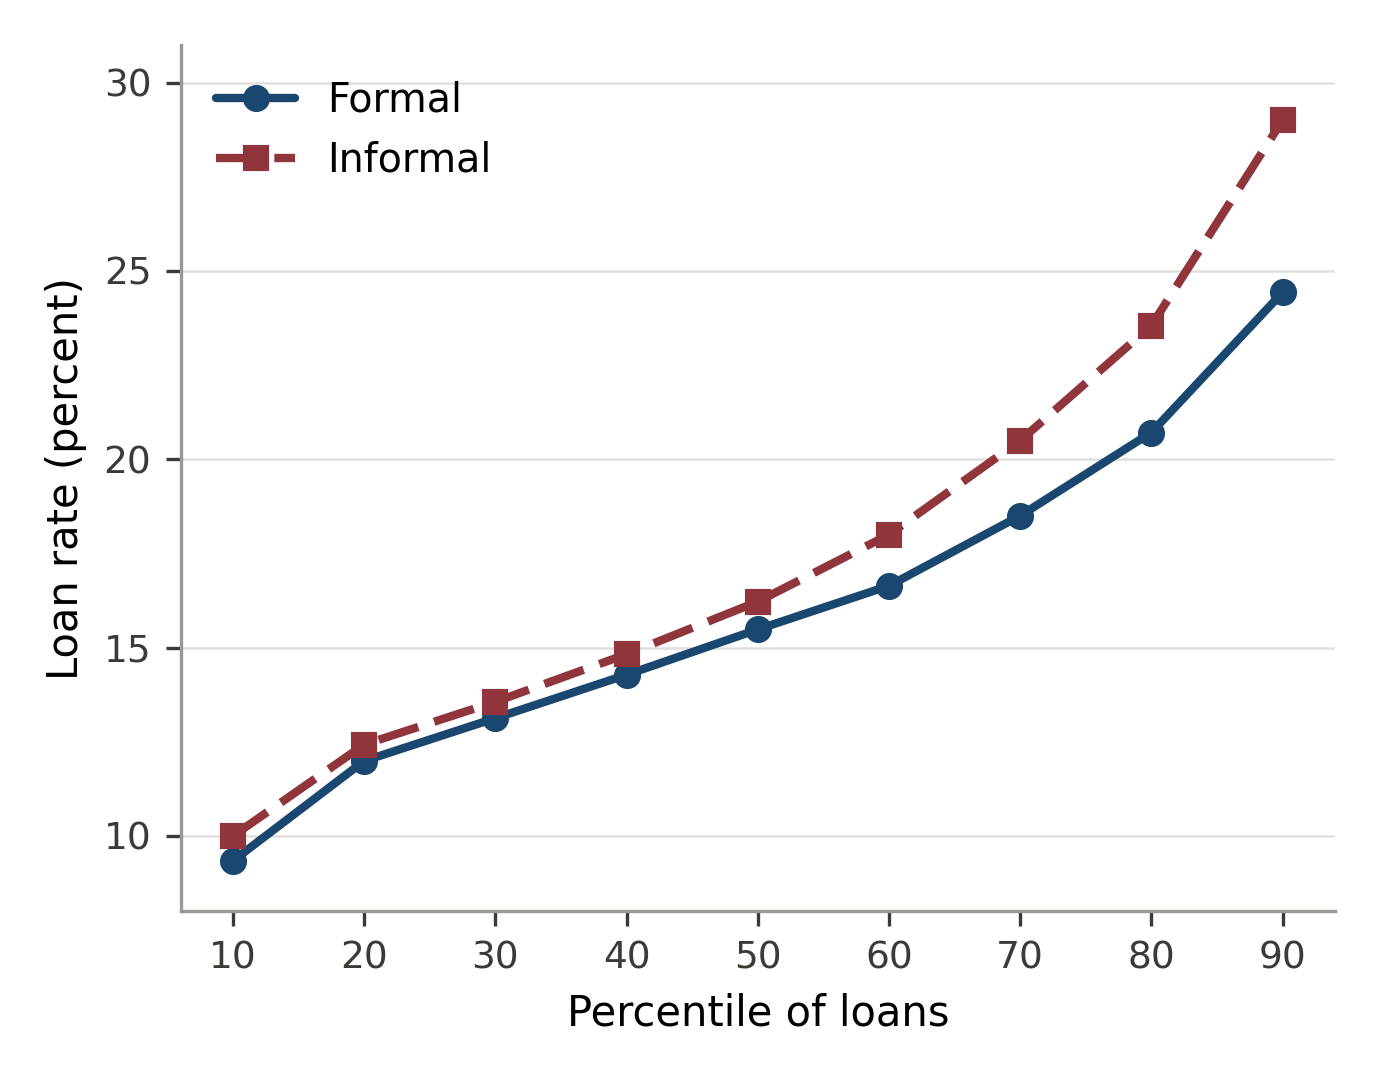
\includegraphics[width=0.62\textwidth]{slides_material/int_rate_pctl_r04.png}
%     \par\footnotesize Percentiles of registry loan rates for formal and informal borrowers, unweighted. A borrower is informal if it has no IMSS employer registration in the loan year. Figure~\ref{fig:inf_validation} in Appendix~\ref{transitions_alternative} compares this classification with the census.
% \end{figure}



\begin{table}[H]
\centering
\caption{Estimation sample: local markets across five year windows}
\label{tab:desc_sample}
\begin{threeparttable}
\small
\setlength{\tabcolsep}{5pt}
\renewcommand{\arraystretch}{0.9}
\begin{tabular}{l r r r r r r}
\toprule
 & Mean & SD & p10 & Median & p90 & N \\
\midrule
\multicolumn{7}{l}{\textit{Panel A. Pooled levels at the start of the window, per market}} \\
All firms & 8,874.6 & 29,241.7 & 415 & 2,319 & 20,316 & 1,394 \\
\quad Formal & 1,094.3 & 3,872.7 & 13 & 138.5 & 2,695 & 1,394 \\
\quad Informal & 7,780.3 & 25,628.2 & 393 & 2,159.5 & 17,436 & 1,394 \\
Firms with bank credit (census) & 572.8 & 1,793.1 & 3 & 119 & 1,331 & 1,394 \\
Switchers, informal to formal & 253.4 & 879.8 & 3 & 38.5 & 589 & 996 \\
Switchers, formal to informal & 229.0 & 814.4 & 3 & 37 & 537 & 996 \\
Borrowers (registry) & 556.8 & 3,714.0 & 4 & 50.5 & 919 & 1,394 \\
Total authorized credit$^{\dagger}$ & 431.5 & 5,578.9 & 0.1 & 2.5 & 195.6 & 1,394 \\
Collateral ratio & 2.21 & 55.35 & 0.00 & 0.04 & 0.31 & 1,394 \\
Interest rate (percent) & 14.86 & 4.56 & 8.88 & 14.91 & 20.30 & 1,394 \\
IMSS workers & 26,655 & 142,866 & 37 & 1,316 & 47,088 & 1,394 \\
\addlinespace[3pt]
\multicolumn{7}{l}{\textit{Panel B. Instrument}} \\
Shift share instrument (standardized) & 0.248 & 1.197 & $-$0.893 & $-$0.261 & 2.063 & 1,394 \\
Coverage & 0.921 & 0.110 & 0.762 & 0.967 & 1.000 & 1,394 \\
\bottomrule
\end{tabular}
\begin{tablenotes}[flushleft]
\footnotesize
\item \textit{Notes:} All statistics pool the 1,394 market window observations (556 markets, windows 2009--2014, 2014--2019, 2019--2024), unweighted. N smaller where undefined. Census is the source for firms by status and firms with bank credit. The registry os the source for borrowers, credit, collateral ratio and interest rate (credit weighted market averages). $^{\dagger}$ Million dollars at 19 pesos per dollar. Coverage: share of baseline credit held by banks with an estimated shock. Five year changes of every outcome, and the full versions by source is in Tables~\ref{tab:desc_sample_census} and~\ref{tab:desc_sample_registry}.
\end{tablenotes}
\end{threeparttable}
\end{table}

\section{A parsimonious model of formality and finance}
\label{sec:toy}

The objective of this section is to build a parsimonious model that rationalizes the link between banking financial conditions and firm's formality decisions. The model is a stationary firm dynamics model in the tradition of \citet{hopenhayn1992entry}, with two operating regimes as in \citet{ulyssea2018firms} and costly external finance as in \citet{gomes2001financing}. We let the empirical facts observed in the data (Section~\ref{sec:descriptives}) to guide our modeling decisions. For instance, we allow firms to switch back and forth their formality status, as observed in Table~\ref{firms_transition}, and informal firms to access bank loans (Table~\ref{tab:desc_firms}, panel A and B) under sector-specific loan terms (Table~\ref{tab:desc_firms}, panel B). The model will serve as stepping stone for the empirical strategy presented in Section~\ref{empirical_strategy_section}. This model will proof helpful to grasp the intuition behind the mechanisms at play and to identify which kind of firms are the treated ones when financial conditions change.

\subsection{Environment}
\label{sec:toy-env}

Without loss of generality, let time to be discrete and last two-periods, $t\in\{1,2\}$. The economy is populated by two type of risk-neutral entrepreneurs: incumbents and potential entrants. An incumbent entrepreneur owns a firm that belongs to a (formal or informal) sector $s\in\{i,f\}$ and holds $k_{1}>0$ installed capital at period 1; while a potential entrant entrepreneur is endowed with financial wealth $k_{0}\geq 0$ and may or may not start a firm in sector $s\in\{i,f\}$ in period 2. Every entrepreneur discounts period 2 at factor $\beta\in(0,1)$ and consumes her dividends and the the depreciated capital, which depreciates at rate $\delta\in(0,1)$. We assume that the output is the \textit{numéraire} good, the wage $w$ is exogenous to the firm, and both, output and wages before taxes, are the same for formal and informal firms. These assumptions allows us to focus our attention on the formality transitions caused by financial conditions and are first-order inconsequential for the conclusions. 
 
An active firm in sector $s$ with capital $k$ and labor $\ell$ produces

\begin{equation}
  y \;=\; \theta\, k^{\alpha}\ell^{\nu},
  \qquad \alpha,\nu>0,\qquad \alpha+\nu<1 .
  \label{eq:toy-tech}
\end{equation}

Where the log productivity combines transitory shocks and a permanent component $v$, drawn at birth from $\ln v\sim N(0,\sigma^{2})$ and known to the firm, such that:

\begin{equation}
  \ln\theta_{1} \;=\; \ln v + \varepsilon_{1},
  \quad
  \ln\theta_{2} \;=\; \rho\,\ln\theta_{1} + (1-\rho)\ln v +
  \varepsilon_{2},
  \quad \varepsilon_{t}\stackrel{iid}{\sim} N(0,\sigma_{\varepsilon}^{2}),
  \quad \rho\in(0,1)
  \label{eq:toy-theta}
\end{equation}
 
A formal firm pays a proportional tax $\tau_y\in[0,1)$ on revenue and a payroll tax $\tau_{\ell}\geq 0$ on its wage bill. An informal firm evades both taxes but is exposed to potential fines that rises with size, in the spirit of \citet{ulyssea2018firms}. Therefore, a firm in sector $s$ hires $\ell^{h}$ at the cost

\begin{equation}
  \mathcal{C}_{s}(\ell^{h}) = \begin{cases}
      (1+\tau_{\ell})\,w\,\ell^{h} & \text{if formal, } s = f \\
      w\,\ell^{h}\Big(1+\frac{\ell^{h}}{\eta_{i}}\Big) & \text{if informal, } s = i
  \end{cases}
  \label{eq:gen-Ci}
\end{equation}

where $\eta_{i}>0$. Notice that informal firms therefore save $\tau_{\ell}$ per worker at small scale, however the saving erodes as the firm grows. This makes formality the optimal regime for large firms even absent financial motives. However, for small enough firms, the only advantages of formality are financial and the only advantages of informality are fiscal and its lower fixed costs. Thus, is for this firms that the financial conditions will play a role. Static profits then are

\begin{equation}
    \pi_{s}(\theta,k)=\max_{\ell^{h}\geq0}(1-\tau_{y}^{s})\theta k^{\alpha}(1+\ell^{h})^{\nu}-\mathcal{C}_{s}(\ell^{h})
\end{equation}

with $\tau_{y}^{f}=\tau_{y}$ and $\tau_{y}^{i}=0$. The model excludes on purpose the possibility of the intensive margin of informality, i.e. firms paying payroll taxes only on part of their total work force. This decision is data driven. As Table \ref{transition_intensive} shows, only 0.7 and 5.3 percent of firms used the intensive margin in 2014 and 2019, respectively. Moreover, this margin is sensitive to enforcement and labor cost policy rather than to credit supply.\footnote{Self-employment is possible in this model and happens at the corner solution $\ell^{h}=0$, which that accounts for the mass of owner only firms in the census.}

Wages and taxes are paid within each period out of contemporaneous revenue and wealth. Investment, in contrast, must be paid one period ahead it becomes productive. Therefore, a firm raises external funds, denoted by $a\geq0$, to cover any difference between the cost of desired capital and its internal funds.\footnote{External finance includes a wide range of funding sources. This paper focuses on bank loans and abstracts from the optimal choice of financing instruments. More broadly, the financing-cost function can be interpreted as a reduced-form representation of other sources of costly external finance, provided that their relevant features are captured by the same specification.}. External finance entails a sector-specific cost, so a firm raising an amount $a$ incurs a financing cost of the form

\begin{equation}
  \Phi_{s}(a) \;=\; \phi_{s}\,a , \qquad
  \phi{_i} \;>\; \phi_{f}\;\geq\;0 ,
  \label{eq:toy-fincost}
\end{equation}

which is paid within period and on top of the repayment of the principal. The parameter $\phi_{s}$ is therefore interpreted as the spread in each sector between the marginal cost of external funds and the risk-free rate. The spread in the informal sector is higher because informal firms cannot pledge audited accounts, registered assets, or formal payroll as information collateral, and it is in line with what is observed in the data (Table~\ref{tab:desc_firms}, panel B). 

Besides the sector difference in price, there is a difference in the amount of external funds available to a firm, which are limited by a collateral constraint on the capital being installed. 

\begin{equation}
  a \;\leq\; b_{s}\,k , \qquad 0\leq b_{i} <
  b_{f} < 1 ,
  \label{eq:toy-collateral}
\end{equation} 

This constraint means that lenders only finance a fraction $b_{s}$ of the installed capital. For formal firms this fraction is higher because being formal raises pledgeability, which is consistent with Table/Figure [x].

Hence, the pair $(\phi_{s},b_{s})$ summarizes in a reduce form the financial conditions faced by sector $s$. The empirical results in Section~\ref{results} analyzes the changes in these two parameters by sector and its consequences in formality. Given its importance, all the comparative statics below are taken with respect to these parameters

A firm faces entry, $c^{e}_{s}$, operating,  $c_{s}\geq0, \,\ c_{f}>c_{i} \geq 0$, and switching costs, $c_{if},c_{fi}\geq0$. Additionally, in period two and before producing, a sector-specific exogenous death probability is materialized, $\lambda_{s}\in[0,1), \,\ \lambda{i}\geq\lambda{f}$.\footnote{The inequality $\lambda{i}\geq\lambda{f}$ is consistent with the data observed in Table~\ref{firms_transition}.} 

The timing is presented in detail in Appendix~\ref{app:toy-details}. A summary of the important aspects is described here. At time $1$, and before observing any shock ($\varepsilon_2$ for productivity and $\lambda_s$ for death), a firm or potential firm must choose her next period sector,  $d \in \{\text{out, informal, formal}\}$. In the transition stage a firm choose the next period optimal level of capital $k_2$ and the level of external funding $a \leq b_{s'}k_2$ at cost $\Phi_{s'}(a)$. Then, in period $2$ and after observing the realization of shocks, active firms produce, sell the depreciated capital and pay taxes, wages, and any cost.

The internal funds available for a firm are the operating profit of the previous period plus the resale value of depreciated capital, net of the fixed costs and any other switching or entry fee:


\begin{equation}
  n \;=\;
  \begin{cases}
    \pi{s}(\theta_{1},k_{1}) - c_{s} + (1-\delta)k_{1}
      - c_{ss'}\mathbf{1}_{\{s'\neq s\}},
      & \text{incumbent of sector } s,\\[2pt]
    k_{0} - c^e{s'}, & \text{entrant into } s' ,
  \end{cases}
  \label{eq:toy-n}
\end{equation}

with $c_{ss}\equiv 0$. Then, an exiting incumbent simply consumes $n^{\text{exit}}=\pi{s}(\theta_{1},k_{1})-c_{s}+(1-\delta)k_{1}$ and a non-entrant consumes $k_{0}$. 
 
\subsection{Capital and investment decisions}
\label{sec:investment_problem}

After solving the static labor problem of the firm, we can re-express her profits as

\begin{equation}
    \pi_s(\theta, k) = \Omega_s\, x\, k^{\gamma}, 
\end{equation}

where $\gamma \equiv \alpha/(1-\nu) \in (0,1)$, $x \equiv \theta^{1/(1-\nu)}$ is the profitable index, and $\Omega_{s} \equiv (1-\nu)\,(1-\tau_y^{s})^{\frac{1}{1-\nu}} \left[\frac{\nu}{(1+\tau_{\ell}^{s})w}\right]^{\frac{\nu}{1-\nu}}$ collects the technology, wage, and taxes paid in sector $s$. This expression is useful because now profits are linear in $x$ and the single sufficient statistic in every decision below is the expectation of the profitability index, which is $\hat{x} \equiv E[x_2 \mid \mathcal{I}_1]$. All the statements are formally presented in Appendix~\ref{app:toy-details} and all proofs are collected in Appendix~\ref{app:toy-proofs}.

Consider now the following problem of capital and external funds at the transition stage of a firm that decided to operate next period in sector $s$, with internal funds $n \geq 0$, and an expected profitability index $\hat x$.

\begin{equation}
  G_{s}(\hat x,n) \;\equiv\; \max_{k\geq0}\;
  -k - \Phi_{s}\!\big(a\big) + \beta\Big[(1-\lambda{s})\,\Omega_{s}\hat x\,
      k^{\gamma} + (1-\delta)k\Big], \quad a=\max\{0,k-n\} \leq b_{s}k
  \label{eq:toy-Gdef}
\end{equation}

Therefore, the value of operating in sector $s$ is $U_{s}(\hat x,n)=n+G_{s}(\hat x,n) -\beta(1-\delta_{s})c_{s}$. In other words, the entrepreneur consumes $n$ minus the resources put into the firm and expects profit net of the fixed cost if it survives plus the depreciated capital resale.

Define the cost of capital as $R^0 \equiv 1-\beta(1-\delta)$ when is acquired with internal funds and as $R_{s} \equiv R^0+\phi{s}$ when capital is paid for with external funds borrowed under sector $s$ conditions. Then, the corresponding optimal capital, $k_s^*(\hat{x}, n)$ targets under these two different prices are
 
\begin{equation}
  \bar{k}_{s}(\hat x)
    = \left[\frac{\gamma \beta(1-\lambda{s})\Omega_{s} \hat x}{R^0}\right]^{\frac{1}{1-\gamma}}
  \quad > \quad
  \tilde{k}_{s}(\hat x)
    = \left[\frac{\gamma \beta(1-\lambda{s})\Omega_{s} \hat x}{R_{s}}\right]^{\frac{1}{1-\gamma}},
  \label{eq:toy-targets}
\end{equation}


Table~\ref{optimal_k_a} summarizes the solution to the capital-financing problem and distinguishes four types of firms. Cash-flow sensitivity refers to the marginal response of optimal capital to internal funds, $\partial k_s^*/\partial n$, holding $\hat{x}$ and $s$ fixed.

\begin{table}[H]
    \caption{Four regions of optimal capital and external funds}
    \label{optimal_k_a}
    \begin{center}
    \renewcommand{\arraystretch}{1.25}\small
    \begin{tabular}{lllll}
        \toprule
         Region & Funds ($n$) vs. $k^{*}_{s}$ & Capital $k^{*}_{s}$ &
         Borrowing $a^{*}_{s}$ & Cash sensitivity \\
        \midrule
        1: Unconstrained & $n\geq\bar k_{s}$ & $\bar k_{s}(\hat{x})$
         & 0 & 0 \\
        2: Constrained & $\tilde k_{s}\leq n<\bar k_{s}$ &
         $n$ & 0 & 1 \\
        3: Borrower & $(1-b_{s})\tilde k_{s}\leq n
         <\tilde k_{s}$ & $\tilde k_{s}(\hat{x})$ & $\tilde k_{s}-n$
         & 0 \\
        4: Collateral-constrained & $n<(1-b_{s})\tilde k_{s}$ &
         $\dfrac{n}{1-b_{s}}$ & $b_{s}k^{*}_{s}$ &
         $\dfrac{1}{1-b_{s}}$ \\
        \bottomrule
    \end{tabular}
\end{center}
\end{table}

The first type is an unconstrained firm with sufficient internal funds to finance its internally financed capital target ($n\geq\bar{k}_s$). This firm does not borrow, and its cash-flow sensitivity is zero. The second type is a constrained non-borrower. Its internal funds are insufficient to attain the internally financed capital target, but borrowing is not optimal. The firm therefore invests all its internal funds, so its cash-flow sensitivity is one because each additional unit of internal funds increases capital by one unit. The third type is a borrower that attains the capital target associated with the higher cost of external finance. It borrows the difference between its chosen capital expenditure and its internal funds. Its cash-flow sensitivity is zero because additional internal funds reduce borrowing without changing its capital choice. The fourth type is a collateral-constrained firm. This firm borrows up to its collateral limit and invests less than its externally financed capital target. Its cash-flow sensitivity is $1/(1-b_s) > 1$. Each additional unit of internal funds supports $1/(1-b_s)$ additional units of capital, including $b_s/(1-b_s)$ units financed through additional borrowing. Finally, notice that the borrowing incidence rises with expected productivity and falls with internal funds. Appendix~\ref{app:toy-details} states the full policy and its derivatives. 
 
\subsection{Sector decision}
\label{sec:toy-sorting}

Define the origin $o \in$ \{out, informal-incumbent, formal-incumbent\}, the destination $d \in$ \{out, informal, formal\}, and the internal funds available before paying the origin-specific fee of each destination as $n_{o}$. Thus, the destination $s$ leaves internal funds $n_{o,s}=n_{o}-\kappa_{os}$ inside the firm, where $\kappa_{os}\in\{c^e_{s},c_{i f},c_{f i},0\}$ per \eqref{eq:toy-n}. Then, the firm's formality decision compares

\begin{equation}
  \Delta_{o}(\hat x,n_{o}) \;\equiv\;
  U_{f}(\hat x,n_{o}-\kappa_{of})
  -U_{i}(\hat x,n_{o}-\kappa_{oi}) .
  \label{eq:toy-Delta}
\end{equation}

There is a unique threshold above which a firm in origin $o$ with internal funds $n_o$ decides to be formal and is defined as $\hat x_o^{if}: \Delta_{o}(\hat x_o^{if},n_{o}) = 0$ (Appendix~\ref{app:toy-details}). More in general, for each origin $o$ and a pair of destinations $d, d'$ there exists a unique productivity threshold that makes one of the destination optimal\footnote{Appendix~\ref{app:toy-details} states the conditions under which the order, unicity and existence of these thresholds hold. In particular, Assumption~\ref{ass:A1} requires that the financing advantage of formality outweighs its fiscal cost net of the survival advantage.}. Define the productivity threshold between origin $o$ and two destinations $d$ and $d'$ as $\hat x_o^{dd'}$. Then we can order each threshold in the expected productivity line such that $ \hat x_i^{oi} < \hat x_o^{oi} < \hat x_f^{oi} < \hat x_f^{if} < \hat x_o^{if} < \hat x_i^{if} $. Table~\ref{threshold} summarizes these thresholds

\begin{table}[H]
    \caption{Four regions of optimal capital and external funds}
    \label{threshold}
    \begin{center}
        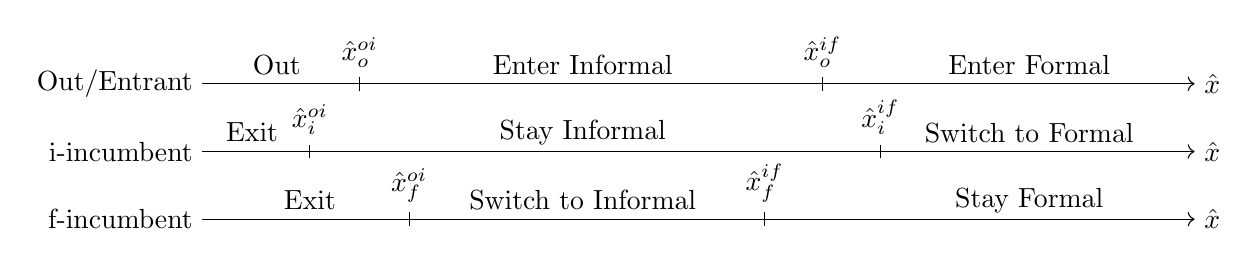
\begin{tikzpicture}[xscale=1.05, yscale=0.86, every node/.style={font=\normalsize}]
          % entrant line
          \draw[->] (0,2) -- (12,2) node[right] {$\hat x$};
          \node[left] at (0,2) {Out/Entrant};
          \foreach \x/\lab in {1.9/{$\hat x_o^{oi}$}, 7.5/{$\hat x_o^{if}$}}
            \draw (\x,1.9) -- (\x,2.1) node[above] {\lab};
          \node at (0.9,2.28) {Out};
          \node at (4.6,2.28) {Enter Informal};
          \node at (10,2.28) {Enter Formal};
          % informal incumbent
          \draw[->] (0,1) -- (12,1) node[right] {$\hat x$};
          \node[left] at (0,1) {i-incumbent};
          \foreach \x/\lab in {1.3/{$\hat x_i^{oi}$}, 8.2/{$\hat x_i^{if}$}}
            \draw (\x,0.9) -- (\x,1.1) node[above] {\lab};
          \node at (0.6,1.28) {Exit};
          \node at (4.6,1.28) {Stay Informal};
          \node at (10,1.28) {Switch to Formal};
          % formal incumbent
          \draw[->] (0,0) -- (12,0) node[right] {$\hat x$};
          \node[left] at (0,0) {f-incumbent};
          \foreach \x/\lab in {2.5/{$\hat x_f^{oi}$}, 6.8/{$\hat x_f^{if}$}}
            \draw (\x,-0.1) -- (\x,0.1) node[above] {\lab};
          \node at (1.3,0.28) {Exit};
          \node at (4.6,0.28) {Switch to Informal};
          \node at (10,0.28) {Stay Formal};
        \end{tikzpicture}
    \end{center}
\end{table}

So far we have established two separated implications of the model. The first one was an anatomy of financially constrained firms based on the firm expected productivity and her internal funds. The second fact was an endogenous sector sorting based on the expected productivity of the firm. However, the relevant predictions of the model are in the interaction of these two implications. To see this, notice that for borrower and collateral-constrained firms (regions three and four in Table~\ref{optimal_k_a}) the sector productivity threshold depends on the financial conditions (parameters $\phi_s$ and $b_s$), this is $\hat x_o^{dd'}(\phi_s,b_s,\phi_{s'},b_{s'})$ $\forall o,d,d',s,s' \in $ \{out, informal, formal\}.

Let $D_o \equiv (\phi_i - \phi_f) n_{o} + (1+\phi_{f})\,\kappa_{of} - (1+\phi_{i})\,\kappa_{oi} + \beta\big[(1-\lambda_{f})c_{f} -(1-\lambda_{i})c_{i}\big] $ and $\Psi_{s}(\hat x;R)\equiv(1-\gamma)\,\gamma^{\frac{\gamma}{1-\gamma}} \big(\beta(1-\lambda{s})\Omega_{s} \hat x\big)^{\frac{1}{1-\gamma}}R^{-\frac{\gamma}{1-\gamma}}$, then for borrowing (borrowers and collateral-constrained) firms, Table~\ref{comparative_stats} summarizes how each sector threshold react to changes in the financial conditions. 

\begin{table}[H]
    \caption{Comparative-statics of sector thresholds with respect to financial conditions}
    \label{comparative_stats}
    \begin{center}
        \small
        \renewcommand{\arraystretch}{1.7}
        \begin{tabular}{lcccc}
            \hline
             & $\phi_{f}\uparrow$ & $\phi_{i}\uparrow$
             & $b_{f}\uparrow$ & $b_{i}\uparrow$ \\
            \hline
            Formality margins
            $\hat x^F_{e},\hat x^F_{i},\hat x^F_{f}$ &
            $\dfrac{(1-\gamma)\,a^{*}_{\fml}}{D_{o}}>0$ &
            $-\dfrac{(1-\gamma)\,a^{*}_{i}}{D_{o}}<0$ &
            $\leq 0$ &
            $\geq 0$ \\
            Informal entry/exit $\hat x^E_{i},\hat x^X_{i}$ &
            $0$ &
            $\dfrac{a^{*}_{i}}{\Psi'_{i}}>0$ &
            $0$ &
            $\leq 0$ \\
            Formal exit $\hat x^X_{f}$ &
            $0$ &
            $\dfrac{a^{*}_{i}}{\Psi'_{i}}>0$ &
            $ 0$ &
            $\leq 0$ \\
            \hline
            \multicolumn{5}{@{}p{0.97\linewidth}@{}}{\footnotesize\emph{Note}: entries assume the threshold ordering of Proposition~\ref{prop:ordering}, so the formal incumbent's relevant alternative at its exit margin is the switch-down option; off that ordering the formal-exit row picks up $\geq0$ ($\phi_{f}$) and $\leq0$ ($b_{f}$) terms through the value of staying formal. The first row reports $\partial\ln(\text{threshold})/ \partial(\text{parameter})$; the second and third rows report level derivatives, with $a^{*}_{i}$ evaluated at the margin's funds ($n$ for informal exit/entry, $n-c_{fi}$ for formal exit).}\\
        \end{tabular}
    \end{center}
\end{table}

The results of the model in Table~\ref{comparative_stats} yield testable predictions that will be verified against the empirical results in Section~\ref{results}. The first prediction is that cheaper or more abundant credit in the formal sector (a fall in $\phi_{f}$ or a rise in $b_{f}$) should lower every formality threshold and increase formal entry, more informal-to-formal switching, and less formal-to-informal switching. The second prediction is cheaper or more abundant credit in the informal sector (a fall in $\phi_{i}$ or a rise in $b_{i}$) lowers the thresholds of informal entry, informal exit, and formal exit, which would raise informal entry, lower exit from either sector, reduce formalization, and raise de-formalization. 


Notice that what matters for the model prediction about formality threshold and the size of the transitions is the difference between the financial conditions in the formal and informal sector and the density of firms sitting next to the thresholds, both for intensive loan deepening by continuing borrowers and loans created for new borrowers. Appendix~\ref{app:toy-details} presents the generic closed form and Appendix~\ref{app:estimand} works out the informality-mass case in detail.

Add a Figure [X] with two dimension threshold: productivity and internal funds.

% The model, finally, makes precise what the Leave-One-Out Shift-Share coefficient identifies through the lens of the model: to first order, the model counterpart of the IV estimand is the ratio of two equilibrium responses to the same financial-conditions shift, a density-weighted sum of threshold shifts in the numerator over a denominator that mixes intensive loan deepening by continuing borrowers with loans created and swapped at the margins. Appendix~\ref{app:toy-details} presents the generic closed form and Appendix~\ref{app:estimand} works out the informality-mass case in detail. Three lessons carry, first, the IV coefficient is large where many firms sit near their thresholds, which rationalizes why the gross-flow elasticities exceed the net stock response, flows add up threshold crossings while the stock nets them out, and why the responses concentrate on the formal side, the sector whose borrowing terms the shock improves. 

% Proposition~\ref{prop:statics} carries three observations. First, cheaper or more abundant formal credit (a fall in $\phi_{f}$ or a rise in $b_{f}$) lowers every formality threshold. This produces more formal entry, more informal-to-formal switching, and less formal-to-informal switching. It leaves the formal exit margin unchanged, because the exiting formal firm's relevant alternative is the switch-down option, and formal-side terms do not enter it. This is the pattern of the IV estimates: formal entry and formalization rise, and de-formalization falls. Second, cheaper or more abundant informal credit (a fall in $\phi_{i}$ or a rise in $b_{i}$) lowers the informal entry, informal exit, and formal exit thresholds. It would raise informal entry, lower exit from either sector, reduce formalization, and raise de-formalization. The estimates show none of these movements, informal entry is flat and exit rises, so the data assign the shock a predominantly formal-side incidence. The structural estimation of Section~\ref{sec:estimation} agrees: the informal-side loading of the shock is small but positive, about two thirds of the formal loading. Third, all effects are zero for unconstrained firms. They are proportional to equilibrium borrowing at the margin for constrained firms, and hence concentrated on firms with high growth needs relative to internal funds.
 
% A remark on what this implies for the general quantitative model. The exact zeros in the table are exclusion restrictions delivered by the two-period structure. However, with an infinite horizon, continuation values embed the option to switch sectors again later, so a formal-side parameter leaks into an informal continuation value at second order (and conversely). The general model therefore preserves the table's sign pattern and its near-diagonal loading, each margin responds first and foremost to its own sector's terms, in proportion to marginal borrowing, but not the literal zeros. Section~\ref{sec:estimation} verifies exactly this at the estimated parameters, by reporting the full Jacobian of moments with respect to parameters: the quantitative counterpart of this table.
 
\section{Empirical strategy} \label{empirical_strategy_section}

\subsection{Shift-Share identification with exogenous shocks}

We are interested in estimating the impact of credit supply shocks on firm-level transitions (formality status, entry, and exit) and other outcomes. The problem is that OLS estimates are contaminated by reverse causality and omitted-variable bias: markets with more informal-to-formal transitions may demand more credit, and an unobserved technology shock may simultaneously raise firm entry and credit volumes.

A Shift-Share design with an exogenous shifter overcomes this endogeneity. Consider the ideal experiment where additional funding is randomly allocated across banks, raising the credit supply of the selected banks. Because the selection is random, it is uncorrelated with firms' demand for credit and, hence, with firm transitions and other outcomes. In this setting, identification requires, as an exclusion restriction, that the lottery affect outcomes only through credit in equilibrium.

For these reasons, we implement a Leave-One-Out Shift-Share Instrumental Variable (LOO-SSIV) approach, following \citet{amiti2018much} and \citet{greenstone2020credit}. First, we decompose yearly bank-firm credit growth into demand and supply components. We exclude from the sample the market $m$ that we are interested in (the Leave-One-Out step) to eliminate the mechanical bias that would arise from estimating $\hat{\gamma}_{bt}^{-m}$ on data that include market $m$'s own observations. Specifically, we estimate

\begin{equation} \label{fe}
    \Delta \ln L_{bft} = \alpha_{ft}^{-m} + \gamma_{bt}^{-m} + \epsilon_{bft}^{-m},
\end{equation}

where $\Delta$ denotes the one-year log change, $\alpha_{ft}^{-m}$ is a firm-year fixed effect that absorbs credit demand, and $\gamma_{bt}^{-m}$ is a bank-year fixed effect that recovers the bank-specific supply shock.
The regression is weighted by the total credit authorized from the bank to the firm over the five preceding years and the estimated bank-year effects are normalized to have zero mean within each year. Finally, we add the yearly shocks over the five-year window, $\hat{\gamma}_{bt,5}^{-m} = \sum_{k=0}^{4} \hat{\gamma}_{b,t-k}^{-m}$, to match the five year differences of the outcome variables.\footnote{The zero credit-weighted mean of the yearly shocks imply that adding over a year without a valid estimated shock is equivalent to assign to that year the average shock.}

Notice that the estimation relies on the yearly credit variation across banks within a firm, so that only firms borrowing from two or more banks in a given year contribute to the estimation\footnote{From the pool of borrower firm-years, 13\% hold loans from more than one bank and 87\% borrow from a single bank. In terms of loan volume, 66\% comes from multi-bank firms, while 34\% comes from single-bank firms.}. In what follows, we maintain the standard assumption that the supply shock identified on multi-bank firms also applies to single-bank firms. Relaxing this assumption yields similar results, as shown in the robustness exercise in Section \ref{robustness}, where we replace firm-year fixed effects with market-sector-year fixed effects as in \citet{degryse2019identifying}. This change allows single-bank firms to also contribute to identification at the cost of potentially absorbing demand shifters into the estimated supply shocks. To validate that the bank effects capture supply rather than demand, Table~\ref{firm_km_table} in Appendix~\ref{firm_km_section} shows that bank shocks predict within-firm credit changes in the excluded market \citep{khwaja2008tracing}. A one log point higher bank shock raises the firm's credit from that bank by $0.13$ log points relative to its credit from its other banks. At the firm level, the bank shocks affect both single-bank and multi-bank firms ($0.011$ and $0.092$ log points per log point of the share-weighted bank shock), supporting the extension of the supply interpretation to single-bank firms.

Second, we construct bank shares at baseline in each market, 

\begin{equation}
    s_{bm(t-5)} = \frac{L_{bm(t-5)}}{\sum_{b'} L_{b'm(t-5)}},
\end{equation}

and define the Leave-One-Out Shift-Share instrument as

\begin{equation}
    \hat{Z}_{mt}^{LOO} = \sum_{b \in \mathcal{B}_{mt}} s_{bm(t-5)}\, \hat{\gamma}_{bt,5}^{-m},
\end{equation}

where $\mathcal{B}_{mt}$ denotes the set of banks with at least one estimated shock in the window. Following the exogenous-shifter framework of \citet{borusyak2022quasi}, identification requires i) many uncorrelated shocks with dispersed exposure and ii) that the shifters $\hat{\gamma}_{bt,5}^{-m}$ be as-good-as-randomly assigned across banks conditional on the included controls. 

The as-good-as-random requirement would fail if banks receiving larger supply shocks systematically lend in markets with atypical transition dynamics. For example, if an oil boom simultaneously raises firm entry in oil-intensive markets and lending by oil-specialized banks in those same markets. In this case, the estimated coefficient would partly capture sectoral demand rather than credit supply. We address these concerns by including controls that may correlate with both the shifter and the outcome (most directly, the market's sectoral composition of employment and of the lending banks' portfolios) and by conducting a battery of robustness checks (Section~\ref{robustness}). 

The many-uncorrelated-shocks condition requires exposure to be dispersed across many effectively independent bank shocks. In our context, the Mexican banking system is highly concentrated. Table~\ref{shock_stats} shows that the effective sample size, $\mathrm{ESS}=1/\sum_{b,t} w_{bt}^{2}$, in the pooled period is $16.6$ and in the 2014-2019 window a single bank accounts for half of the exposure weight.\footnote{This is the descriptive statistics evidence suggested by \citet{borusyak2022quasi}.} We argue, nevertheless, that this concentration is not a threat to our identification since the estimation does not rest on any single bank, no bank-window carries more than $17\%$ of the pooled exposure weight. Moreover, Section~\ref{robustness} shows the point estimates are robust to dropping the largest bank altogether and to the unweighted specification, at the cost of precision.

\begin{table}[H]
    \caption{Descriptive statistics of the standardized bank shocks}
    \label{shock_stats}
    \centering
    \small
    \begin{threeparttable}
    \begin{tabular}{lccccccccc}
        \toprule
         & \multicolumn{3}{c}{Exposure weighted} & \multicolumn{3}{c}{Unweighted} & & & \\
        \cmidrule(lr){2-4} \cmidrule(lr){5-7}
        Window & Mean & Std. dev. & IQR & Mean & Std. dev. & IQR & Nb. banks & ESS & W \\
        \midrule
        2009-2014 & 0.20    & 0.59 & 1.12 & $-0.23$ & 0.56 & 1.07 & 26 & 8.38  & 0.18 \\
        2014-2019 & 0.14    & 1.53 & 3.05 & 1.07    & 0.88 & 1.00 & 42 & 3.40  & 0.51 \\
        2019-2024 & $-0.35$ & 0.39 & 0.53 & $-0.64$ & 0.49 & 0.38 & 61 & 7.94  & 0.29 \\
        \midrule
        Pooled     & 0.00    & 1.00 & 1.17 & 0.00    & 1.00 & 1.19 & 67 & 16.56 & 0.17 \\
        \bottomrule
    \end{tabular}
    \begin{tablenotes}[flushleft]
        \footnotesize
        \item Notes: The table describes the accumulated five-year bank supply shocks $\hat{\gamma}_{bt,5}$, estimated on the full sample rather than the leave-one-out counterparts used by the instrument, whose only difference is the exclusion of one market at a time. All statistics are computed over the bank-window cells with positive exposure in the estimation sample of the main specification ($1{,}394$ market-years, three five-year windows ending in 2014, 2019, and 2024).
        \item Within each block (exposure-weighted and unweighted), shocks are standardized to zero mean and unit variance over those cells using the corresponding weights, so the pooled means and standard deviations equal 0 and 1 by construction. IQR is the difference between the 75th and 25th percentiles.
        \item The weight $w_{bt}$ is bank $b$'s share of the baseline credit of the estimation sample markets in window $t$, normalized to sum to one within each window for the window rows and across all bank-window cells for the pooled row. ESS $=1/\sum w_{bt}^{2}$ is the effective sample size of the shocks \citep{borusyak2022quasi}. W denotes the largest normalized weight.
        \item Nb. banks counts banks with an estimated shock and positive exposure in each window. The pooled row reports distinct banks (67 banks, across 129 bank-window cells).
    \end{tablenotes}
\end{threeparttable}
\end{table}

Additionally, Section~\ref{robustness} shows the estimates are robust to dropping the largest bank. The left panel of Figure~\ref{fig:maps} displays the instrument on a map, where neighboring markets can be subject to very different magnitudes of the shock, which is where the identifying lies. Moreover, there is no visible geographical relation between the instrument and the baseline informality rate (right panel),\footnote{Figure~\ref{fig:map_credit} in  Appendix~\ref{credit_growth} plots the map of realized credit growth.} for which the balance evidence in Section~\ref{robustness} shows more formal evidence. 

\begin{figure}[H]
    \caption{The identifying variation across local markets}
    \label{fig:maps}
    \centering
    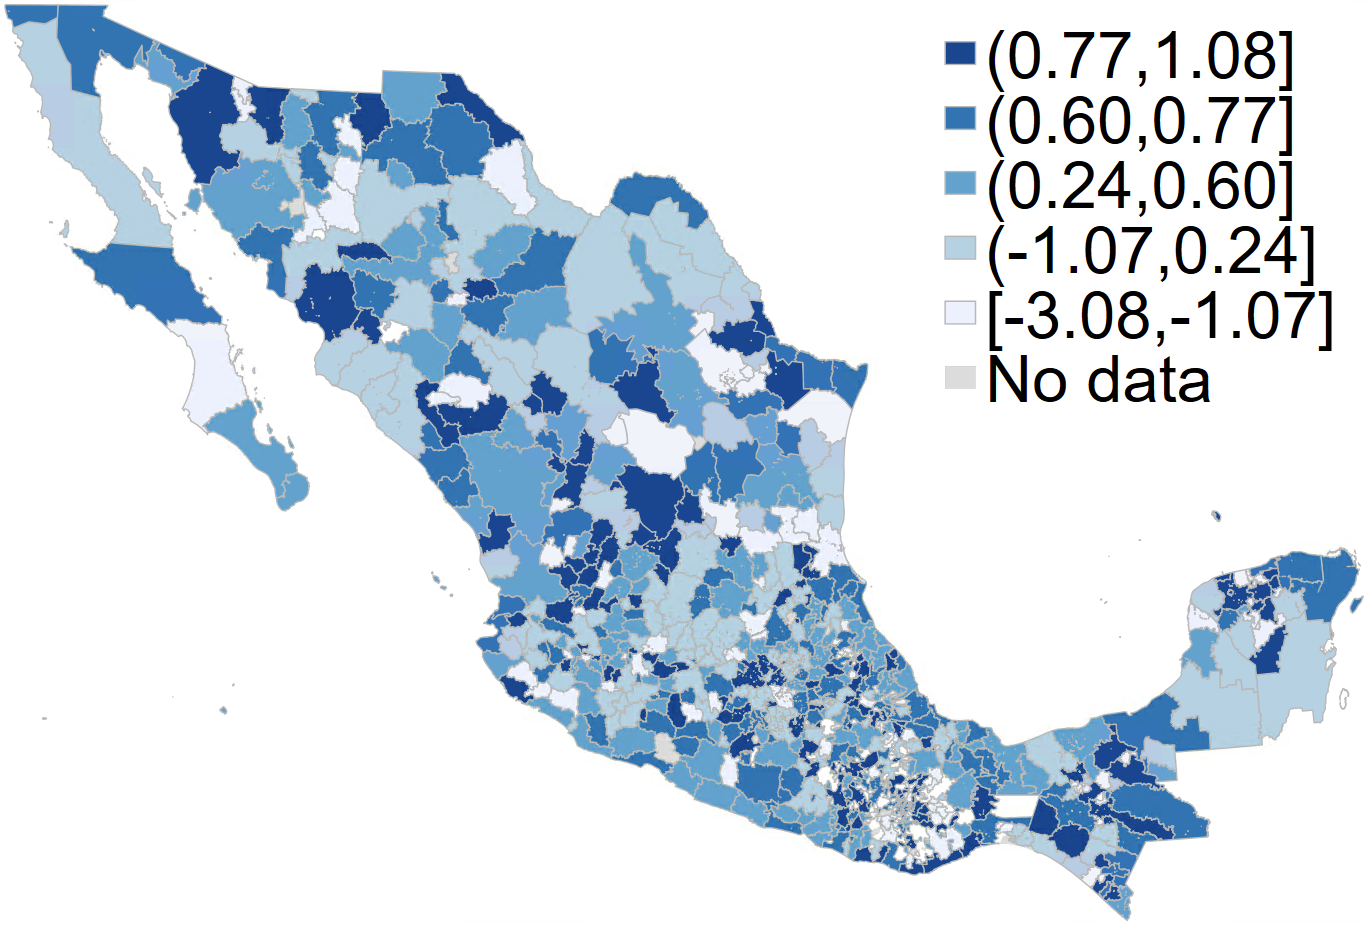
\includegraphics[width=0.48\textwidth]{slides_material/map_iv.png}
    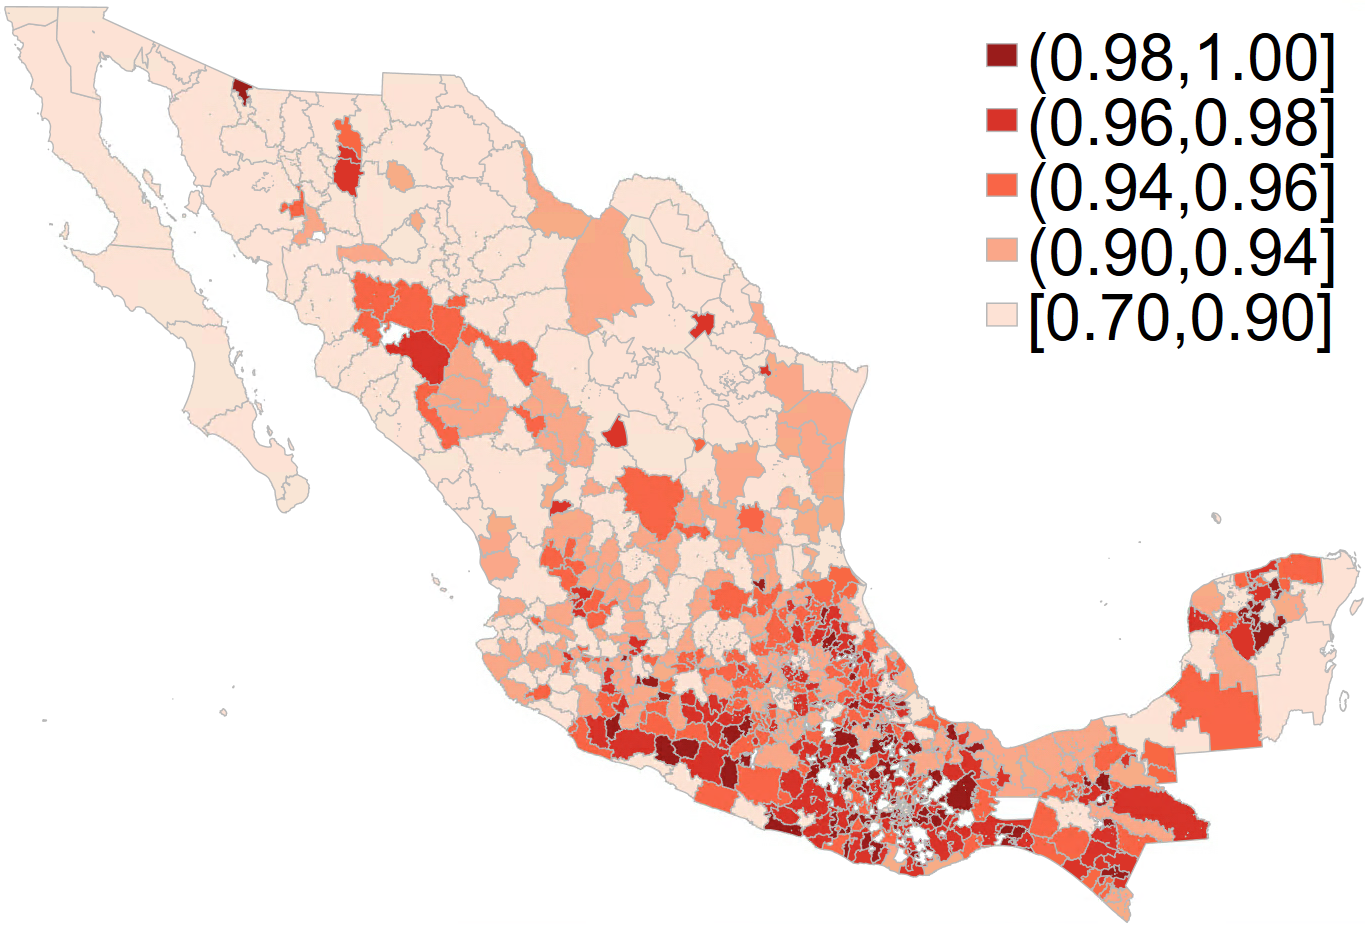
\includegraphics[width=0.48\textwidth]{slides_material/map_informality.png}
    \par\footnotesize The left panel maps the Shift-Share instrument across local labor markets. The right panel maps the baseline informality share. Gray areas have no credit data.
\end{figure}

Once the instrument is built, the main estimating equation that relates local credit growth to outcome variables at the market level is:

\begin{equation} 
    \Delta_5 y_{mt} = \beta \, \Delta_5 \ln(C_{mt}) + X_{m(t-5)}'\Gamma + \lambda_t + \varepsilon_{mt},
    \label{eq:main_iv}
\end{equation}

where $\Delta_5 y_{mt}$ is the five-year change in the outcome (such as the log number of firms by formality status, entry, wages, or value added); $\Delta_5\ln(C_{mt})$ is the five-year log-change in credit in market $m$, instrumented by $\hat{Z}_{mt}^{LOO}$, which is standardized to unit variance; and $\lambda_t$ captures the year fixed effects. The vector $X_{m(t-5)}$ contains the controls (used in every market level regression), which are: the sectoral composition of employment and of the lending banks' portfolios; the credit weighted average interest rate; the log numbers of banks and of loans; the credit share of the market's largest bank; and the sum of exposure shares, which is the share of credit granted by banks with a valid estimated supply shock, interacted with the year fixed effects. This last control accounts for the fact that exposure shares sum to less than one when some banks have no valid estimated supply shock, as prescribed by \citet{borusyak2022quasi} in the presence of incomplete shares. All controls vary at the market level and are fixed at their values at the start of each five year window. Regressions are weighted by the market's baseline credit $C_{m(t-5)}$.

Notice that the specification is estimated in five-year differences with updating exposure shares fixed at the start of each window, rather than in levels with market fixed effects. We choose this specification because, when shares update across windows, unit fixed effects do not isolate shock variation over time, whereas the first difference specification does, and the updating shares keep the first stage strong \citep{borusyak2022quasi}.

Therefore, the corresponding first stage is

\begin{equation}
    \Delta_5 \ln(C_{mt}) = \pi \hat{Z}_{mt}^{LOO} + X_{m(t-5)}'\Pi + \lambda_t + u_{mt}.
    \label{eq:first_stage}
\end{equation}

Some outcomes are available yearly and therefore we analyze their one-year changes, instead of five-year changes. For instance credit, interest rate, and collateral requirements. For this cases, the previous empirical strategy holds replacing every five-year index, change, and accumulation for their one-year counterpart. 

The coefficient of interest is $\beta$ in Equation~\ref{eq:main_iv}, which is the causal elasticity of the outcome with respect to credit at the market level, identified by exogenous bank level supply shocks. The interpretation is that one percent increase in credit supply implies an outcome change of $\hat{\beta}$-percent if the outcome is in logs, or of $\hat{\beta}$/100 percentage point if the outcome is in shares. \citet{adao2019shiftshare} argue that conventional standard errors over-reject in this setting because market residuals are correlated. In other words, markets with similar bank shares are exposed to the same shocks regardless of geographic distance. Following these authors suggestion, we report their exposure-robust standard errors, alongside standard errors clustered by market. 


% $100 \times (1.01^{\hat{\beta}} - 1) \approx \hat{\beta} $ 

% Notice that to maximize the first stage and simultaneously isolate the shock variation over time we will use the first difference specification instead of updating shares (Borusyak, Hull, \& Jaravel, 2020). Moreover, the shock level estimation avoids inferential biases coming from shock exposure (Borusyak, Hull, \& Jaravel, 2020). % If a researcher wants to update the shares to maximize the first stage, but also isolate the shock variation over time (which is not achieved by controlling for unit fixed effects with time-varying shares), she may instead use the first-differenced specification
% (Borusyak, Hull, \& Jaravel, 2020) By estimating a regression at the level of as-good-as-random variation (here, shocks) one avoids inferential biases due to clustering (here, by shock exposure).

% Propotion 1 of (Borusyak, Hull, \& Jaravel, 2020): Equivalence between usual SSIV and shock level IV. Useful because doesn't relies on iid observations (violated if observed and unobserved LLM level shocks).
% Given the equivalence between the Shift-Share IV (SSIV) estimator and the second-stage coefficient from a share weighted shock level IV regression that uses the shocks as the instrument ((Borusyak, Hull, \& Jaravel, 2020), we proceed as follows. First, consider the following residualized dependent and independent variables

% \begin{align}
%     \ln(y_{mt}^{\perp}) = \ln(y_{mt}) - \theta' c_{mt} \\
%     \ln(L_{mt}^{\perp}) = \ln(L_{mt}) - \phi' c_{mt}
% \end{align}

% Where $y_{mt}$ are the variables of interest (log of number of firms in a sector or transitioning) and $c_{mt}$ includes an intercept and controls at the LLM. The controls included are the log of the number of workers as reported in the IMSS-R04 data and the log of the number of credits, both of them interacted with time. 

% Then, we collapse the variables at the shock (bank) level. Let $e_{mt-1}$ be the exposure weight defined as the baseline existing loan in a market and define the exposure mass as 

% \begin{equation}
%     S_{bt} = \sum_m e_{mt} s_{mbt-1}
% \end{equation}

% Thus, the residualized variables defined at the shock level are

% \begin{align}
%     \ln(\bar{y}_{mt}^{\perp}) = \frac{\sum_m e_{mt-1} s_{mbt-1} \ln(y_{mt}^{\perp})}{\sum_m e_{mt-1} s_{mbt-1}} \\
%     \ln(\bar{L}_{mt}^{\perp}) = \frac{\sum_m e_{mt-1} s_{mbt-1} \ln(L_{mt}^{\perp})}{\sum_m e_{mt-1} s_{mbt-1}}
% \end{align}

% Finally, our equation of interest is 

% \begin{equation}
%     \ln(\bar{y}_{mt}^{\perp}) = b_t +\beta \ln(\bar{L}_{mt}^{\perp}) + \eta_2 q_{bt} + u_{bt}
% \end{equation}

% Where, $\bar{L}_{mt}^{\perp}$ is instrumentalized by the standarized bank fix effect, $\hat{\gamma}_{bt}^{std}$, and $q_{bt}$ are bank level controls that include the log of the number of firms that hold a loan relationship with the bank and the loan weighted average of probability of default\footnote{The default probability of each credit is reported as mandated by the \hyperlink{https://www.gob.mx/cms/uploads/attachment/file/1056741/CUB_BD_R04_C-0430-0439_Cr_ditos_comerciales_Vigencia_202201-actual_Actualizaci_n_11_de_febrero_2026.pdf}{R04C regulations}. Let $L_{fbt}$ be the loan from bank b to firm f in time and $DP_{fbt}$ the default probability of firm f with bank b in time t. Then, the loan weighted average probability of default is defined as 
% \[
%     WDP_{bt} = \frac{\sum\limits_f L_{fbt} * DP_{fbt}}{\sum\limits_f L_{fbt}}
% \]
% .}. This equations are estimated with weights $S_{bt}$ and clustered at the bank level. % \textbf{Borusyak, Hull, Jaravel 2020} said that "besides removing confounding variation from the residual (as any control would do), they ($q_{bt}$) can also be viewed as removing such variation directly from the shocks' 

% Importantly, the conventional heteroskedasticity-robust standard error estimation has valid asymptotic inference for $\hat{\beta}$ (Borusyak, Hull, \& Jaravel, 2020).

\section{Main results} \label{results}

\subsection{Annual effects on credit and loan terms} \label{annual}

This section reports the main results of the IV estimates on credit and loan terms at an annual frequency. All the coefficients, standard errors, and specifications are Table~\ref{annual_table} on Appendix~\ref{annual_appendix}. Figure~\ref{fig:event_credit} reports the effect of the standardized IV on the log credit $h$ years before and after the shock. The contemporaneous coefficient is $0.140$ (s.e.\ $0.031$). Therefore, a one standard deviation increase in the supply shock raises the market credit by 14 log points, about 15 percent, in the year of the shock. This means that for a market with the median baseline credit of the sample, 2.5 million dollars, the supply of credit increases roughly 375 thousand dollars. The effect is persistent over time, reaching a coefficient of $0.220$ ($0.053$) two years after the shock and remaining at $0.201$ ($0.052$) four years after. 

\begin{figure}[H]
    \caption{Credit response to a bank credit supply shock}
    \label{fig:event_credit}
    \centering
    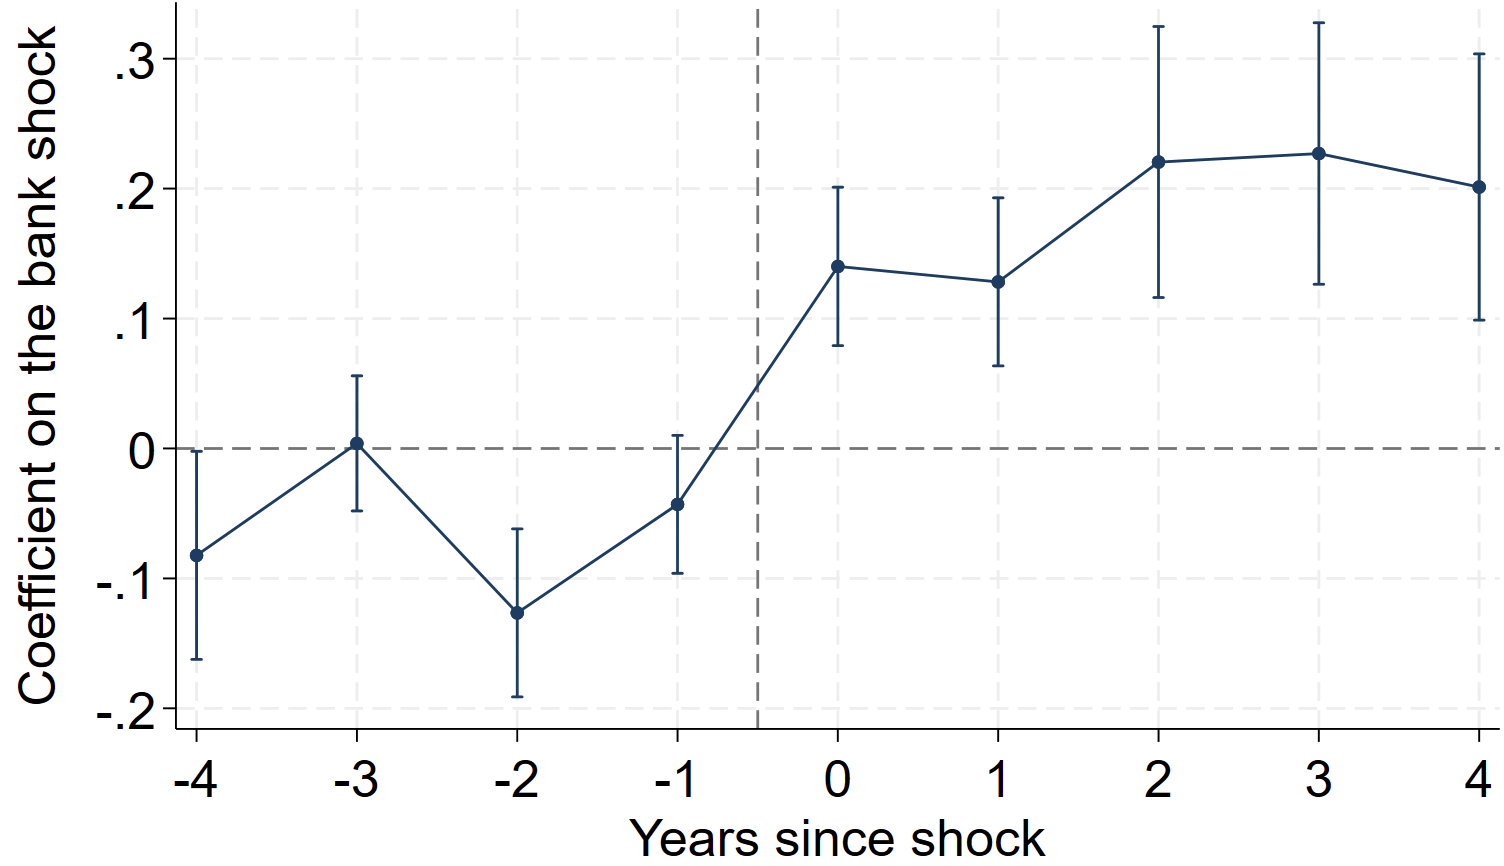
\includegraphics[width=0.495\textwidth]{slides_material/event_cre.png}
        \par\footnotesize \textit{Notes:} Reduced form coefficients on the standardized bank shock from separate annual market level regressions of log credit at each horizon $h$, with the annual analogs of the main controls, weighted by lagged market credit, on market years with instrument coverage of at least 0.5. 95 percent confidence intervals, s.e.\ clustered by market.
\end{figure}

By formality, Figure~\ref{fig:event_credit_fmlty} exposes that the credit supply shock affects the formal sector more strongly. The contemporaneous effect on the formal sector is $0.192$ log points (s.e.\ $0.043$), about 21 percent, which is two and a half times the effect on the informal sector, $0.076$ ($0.030$). This difference, informal minus formal, is statistically significant the first two years of the shock, which falls contemporaneously to $-0.117$ (s.e.\ $0.045$) and $-0.147$ ($0.047$) one year after, both significant at the 5 percent level. However, the gap narrows and is indistinguishable from zero from the second year on. The results support the heterogeneous effect by formality, changing the relative financial advantage of formality.

differentiated effect evidence supports the idea that a bank supply shock changes the relative financial benefits of formality, plausibly causing a re-optimization of the formality decision. 

\begin{figure}[H]
    \caption{Credit response by formality of the borrower}
    \label{fig:event_credit_fmlty}
    \centering
    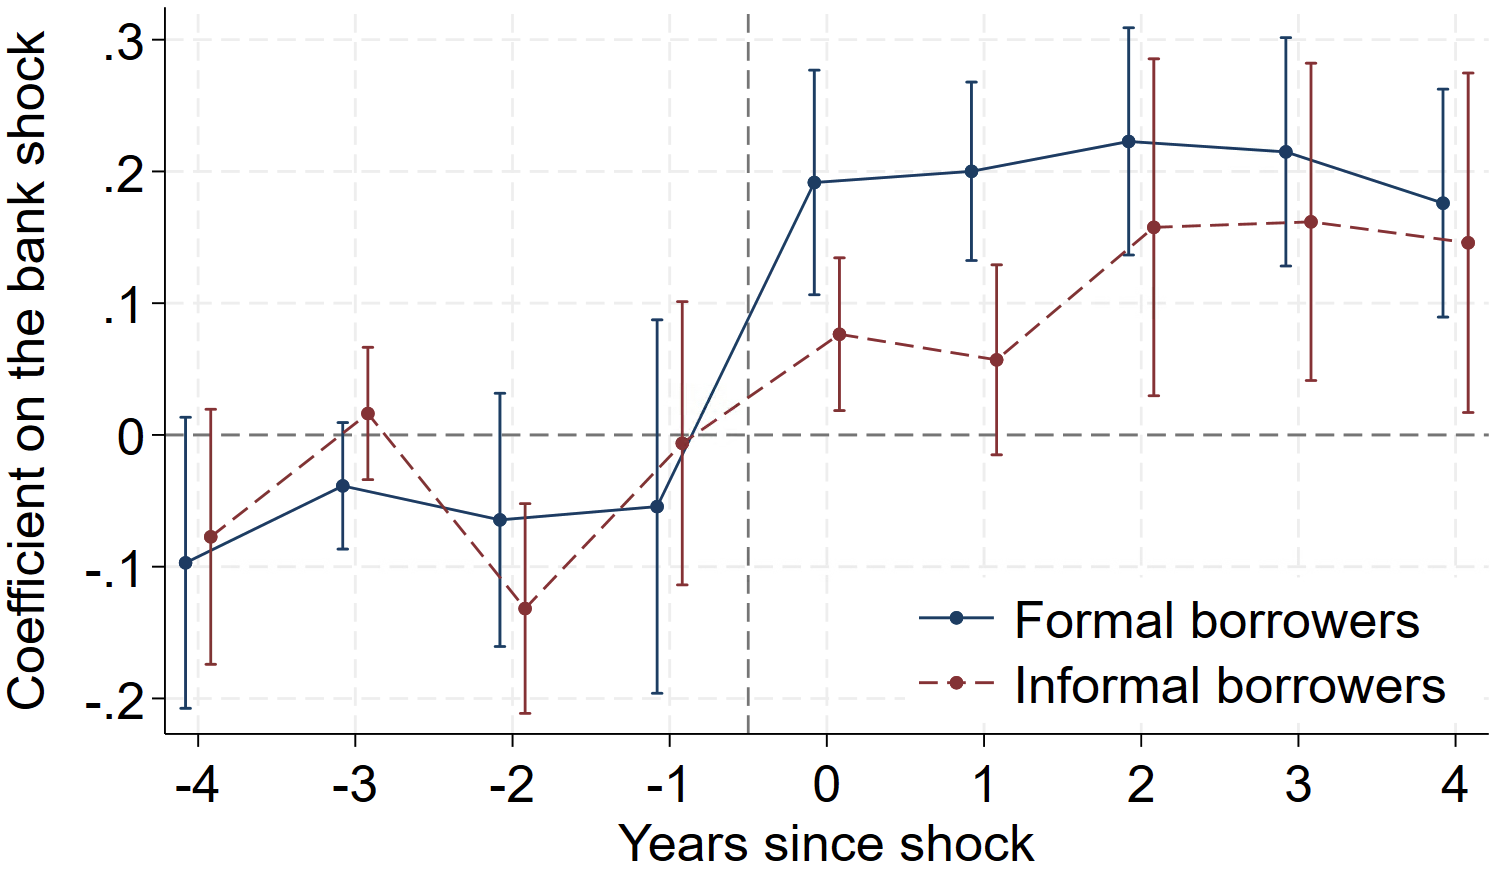
\includegraphics[width=0.495\textwidth]{slides_material/event_cre_frmlty.png}
    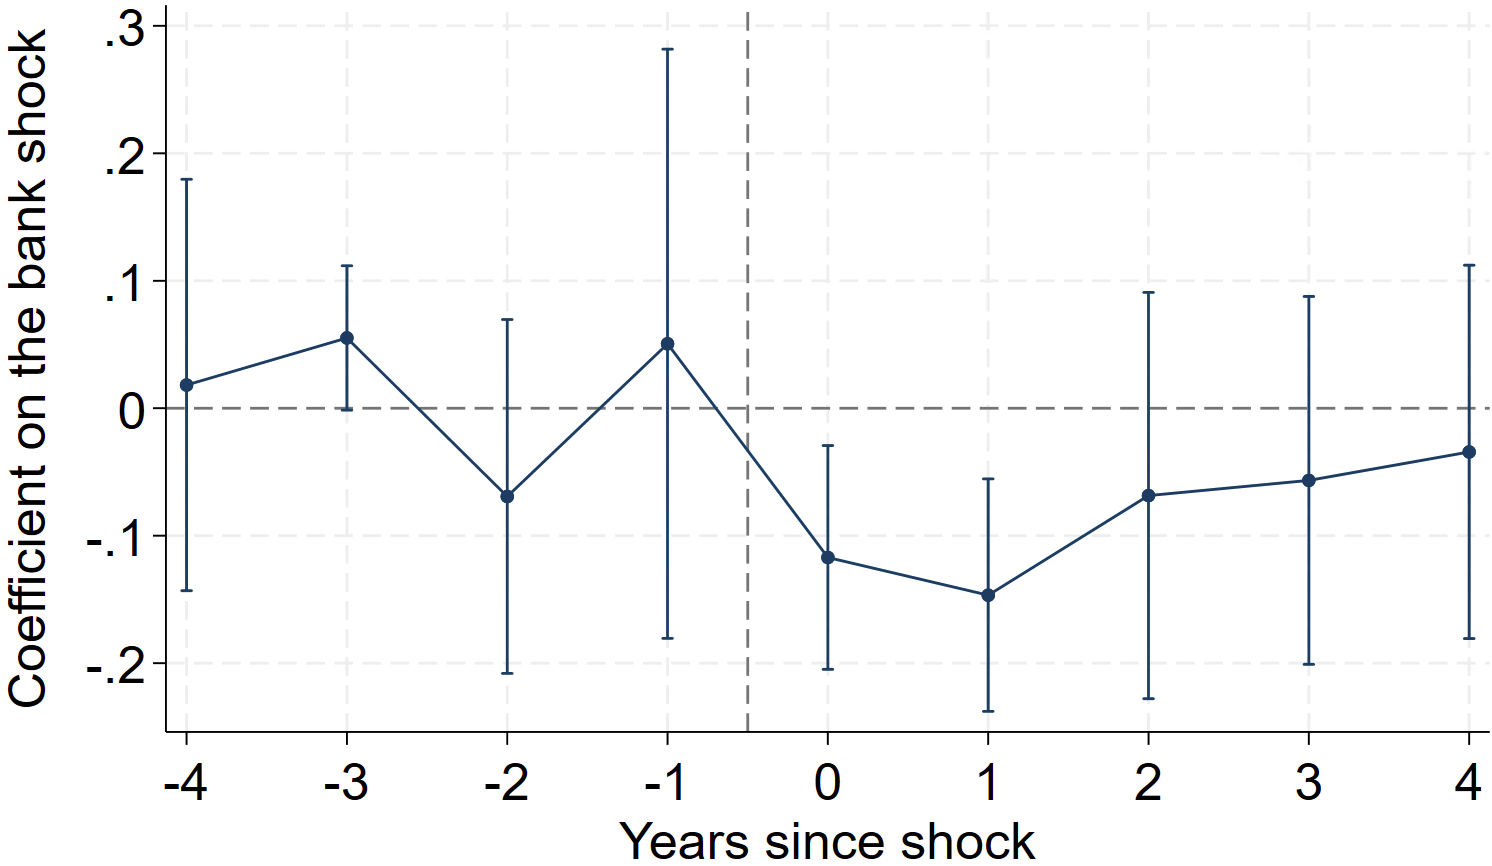
\includegraphics[width=0.495\textwidth]{slides_material/event_cre_df.png}
        \par\footnotesize \textit{Notes:} Same specification as Figure~\ref{fig:event_credit}. Left: log credit to formal and to informal borrowers. Right: difference between the two, informal minus formal, from one regression per horizon on the difference in log credit. 95 percent confidence intervals.
\end{figure}

It has been established that a credit supply shock has a differentiated effect on the volume of credit to formal and informal firms. Now, we investigate if the supply shock has a differentiated effect on the loan terms, like interest rate and collateral requirements. Figure~\ref{fig:event_r_fmlty} displays the response of the lending rate, which falls only for formal firms. For a formal borrower, the rate falls contemporaneously by $0.27$ percentage points (s.e.\ $0.10$) and by $0.52$ ($0.13$) four years later. In contrast, for an informal borrower the rate is unresponsive to the shock, $-0.02$ ($0.11$) the same year and $-0.12$ ($0.12$) four years later. In consequence, the difference, informal minus formal, plotted on the right panel, widens by $0.26$ ($0.14$) percentage points the same year, $0.29$ ($0.13$) one year after and $0.41$ ($0.17$) four years later, significant at the 5 percent level at one, two and four years. This is evidence that the supply shock lowers the price of credit only for formal borrowers, increasing the financial cost advantage of being formal after the shock.


\begin{figure}[H]
    \caption{Interest rate response by borrower formality}
    \label{fig:event_r_fmlty}
    \centering
    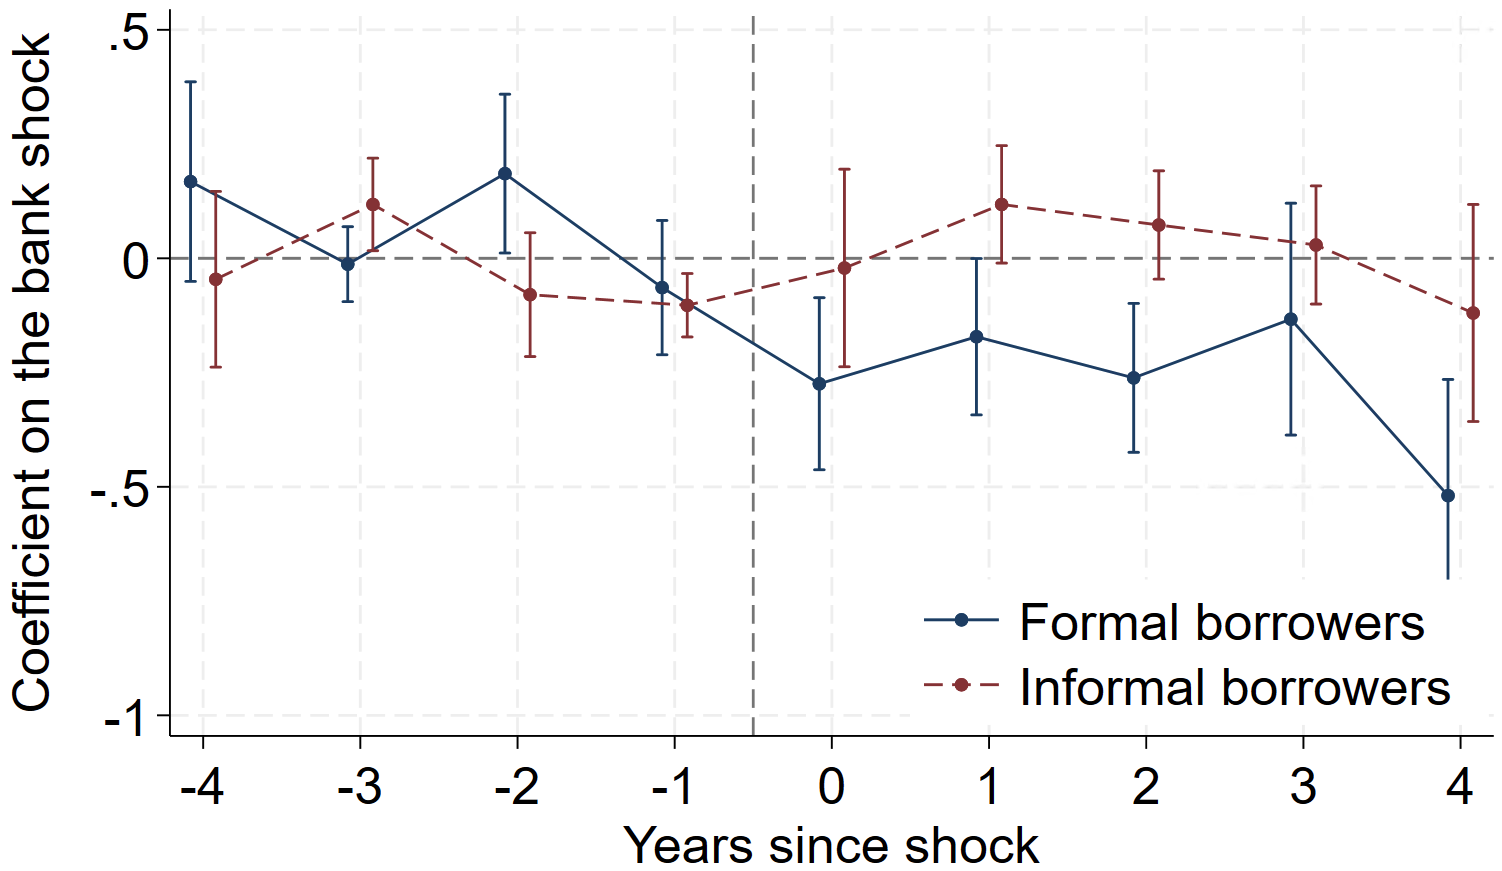
\includegraphics[width=0.495\textwidth]{slides_material/event_r_frmlty.png}
    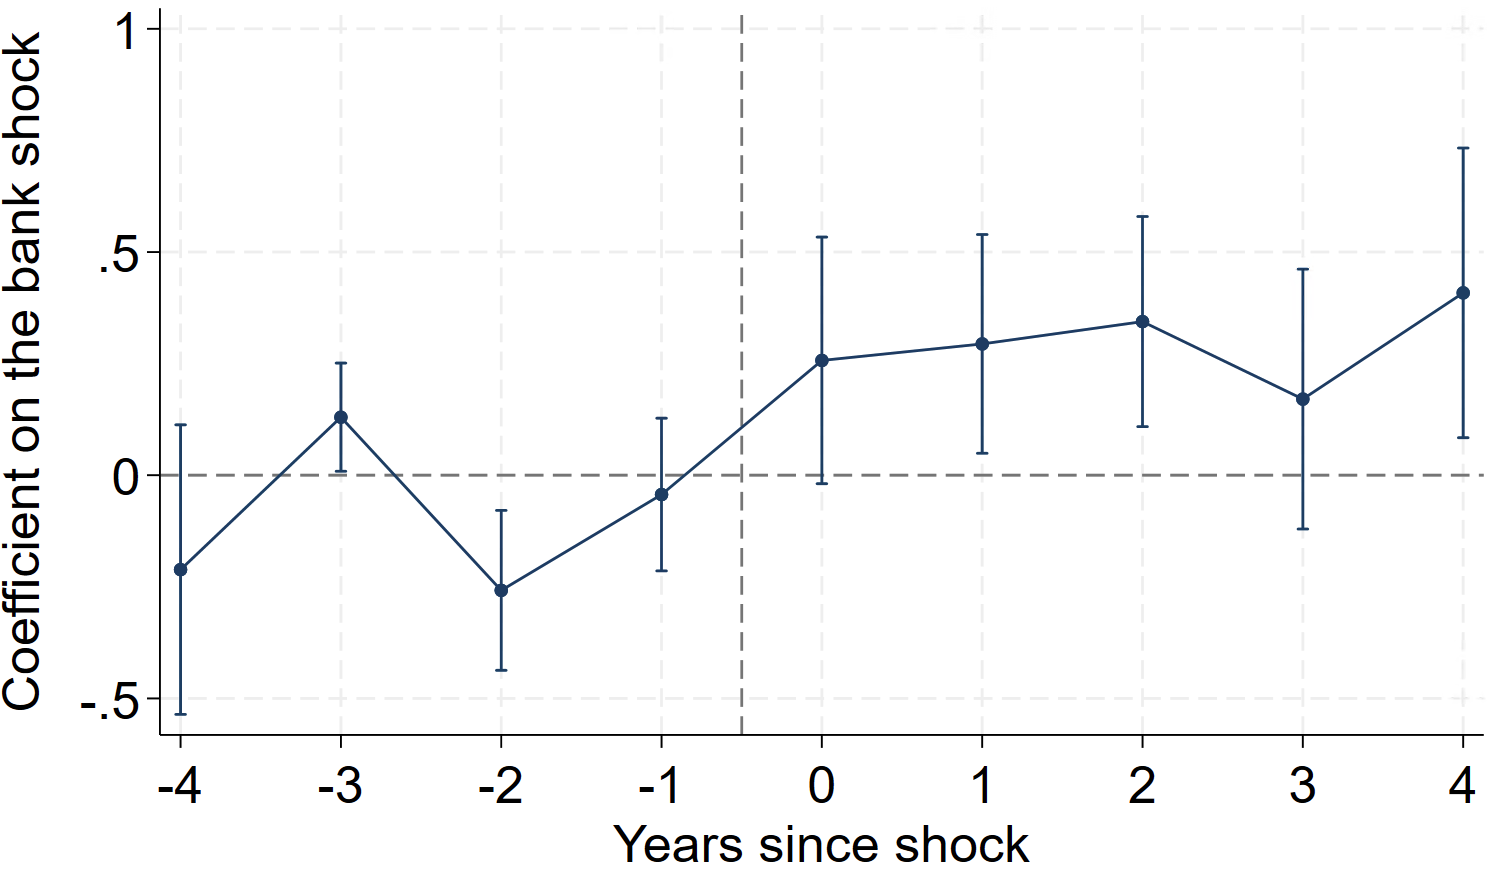
\includegraphics[width=0.495\textwidth]{slides_material/event_r_df.png}
        \par\footnotesize \textit{Notes:} Same specification as Figure~\ref{fig:event_credit}, for the credit weighted lending rate in percentage points. Left: loans to formal and to informal borrowers in the market. Right: difference between the two, informal minus formal, from one regression per horizon. 95 percent confidence intervals.
\end{figure}

Figure~\ref{fig:event_col_fmlty} repeats the exercise for collateral requirements and finds that collateral decreases equally for formal and informal firms after the shock. For a formal borrower, the collateral per peso of credit falls roughly a quarter, by $0.27$ log points (s.e.\ $0.08$) one year after the shock and by $0.29$ ($0.12$) lower four years later. For informal borrowers the fall is marginally smaller, $0.19$ ($0.07$) at two years and $0.14$ ($0.09$) at four. However, this difference is not statistically different from zero, as displayed in the right panel. Hence, the shock relaxes collateral for both groups, with no detectable difference by formality.

\begin{figure}[H]
    \caption{Collateral response by borrower formality}
    \label{fig:event_col_fmlty}
    \centering
    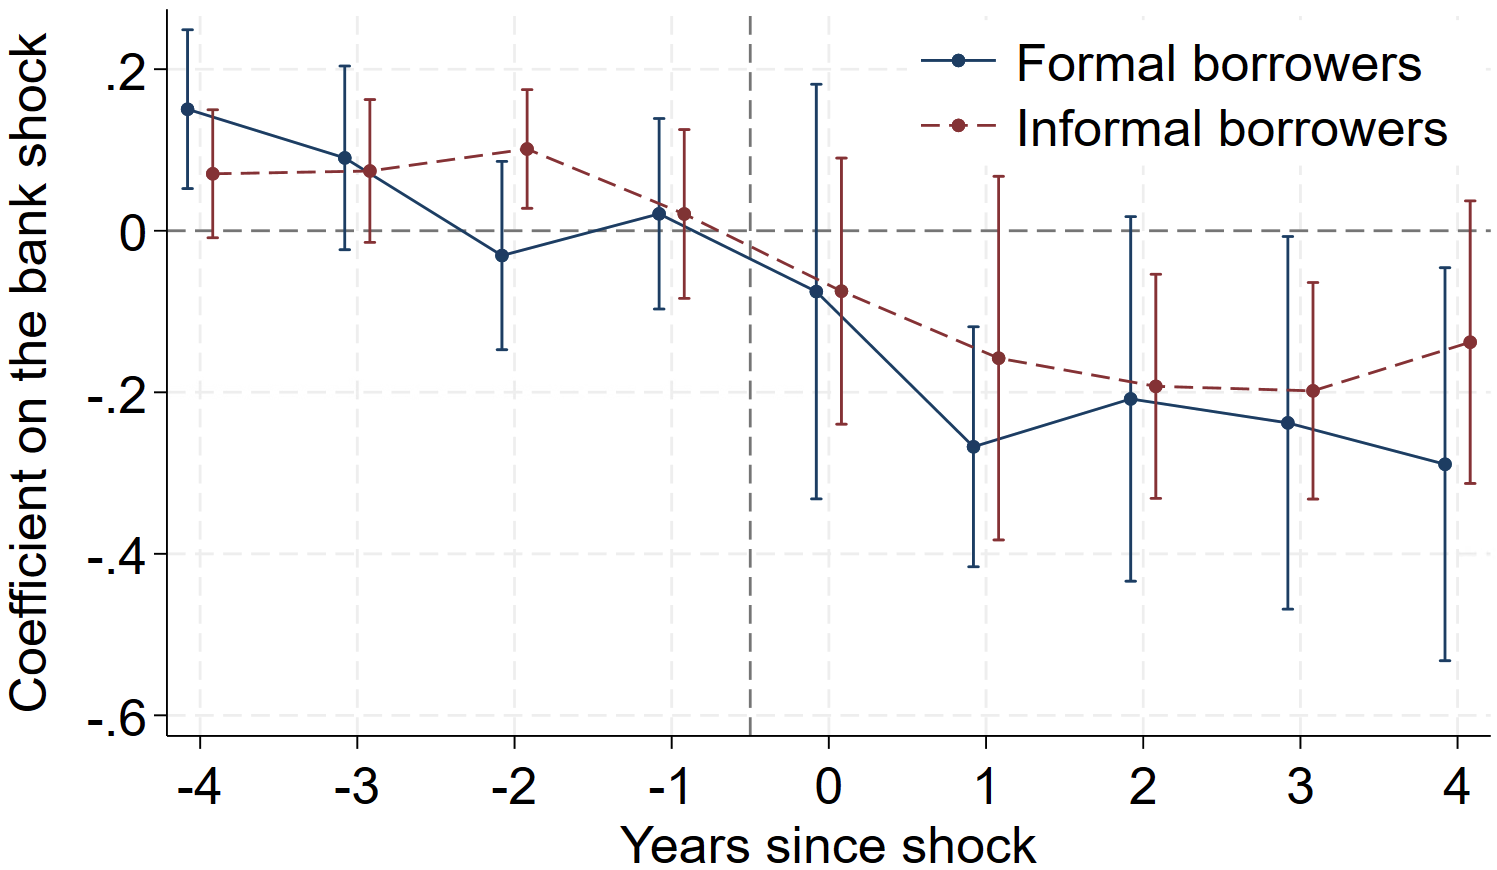
\includegraphics[width=0.495\textwidth]{slides_material/event_col_frmlty.png}
    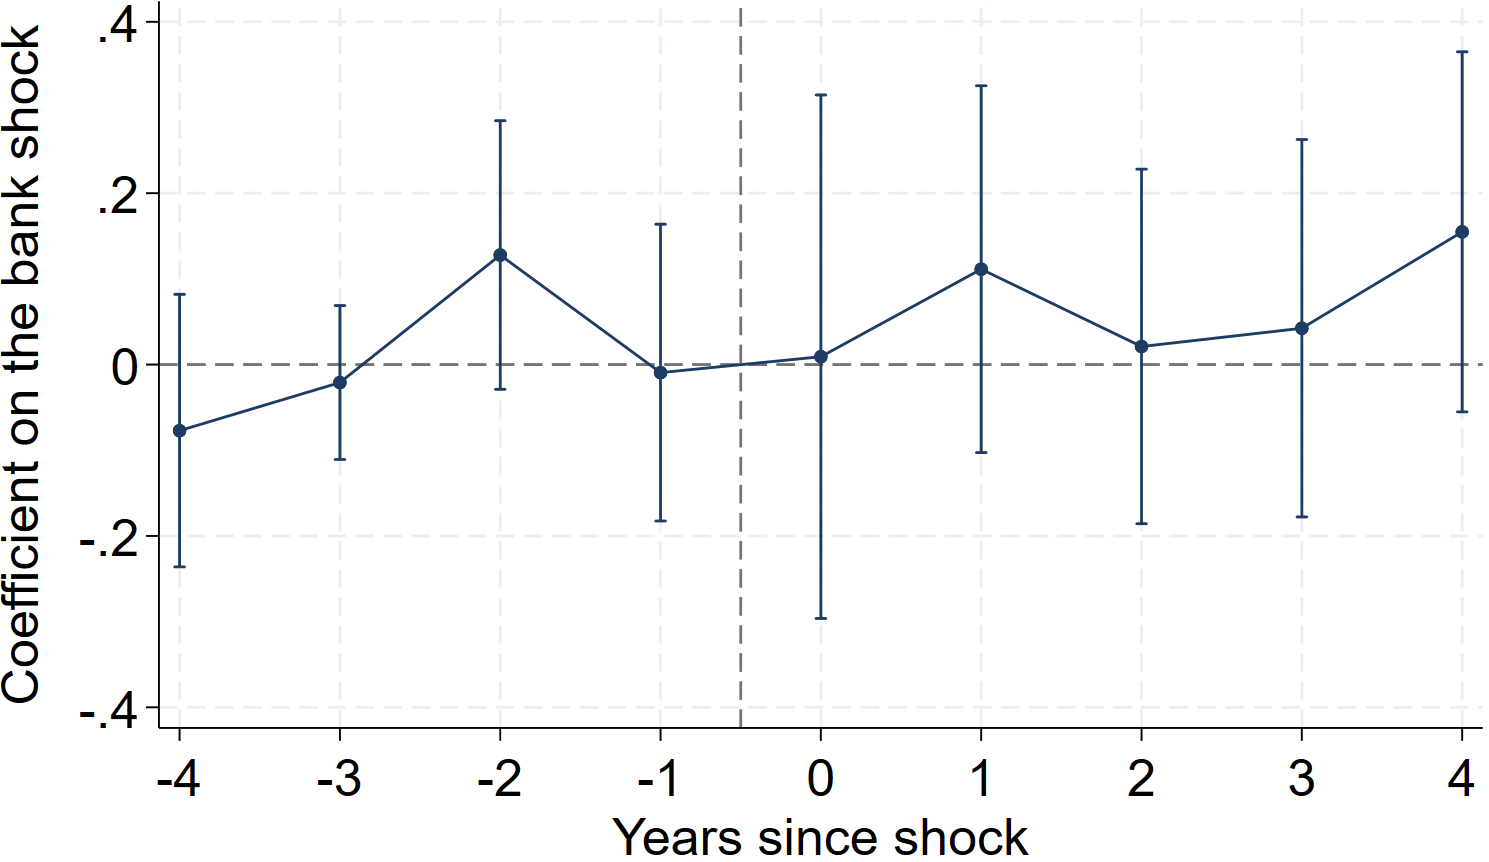
\includegraphics[width=0.495\textwidth]{slides_material/event_col_df.png}
        \par\footnotesize \textit{Notes:} Same specification as Figure~\ref{fig:event_credit}, for log collateral posted per peso of credit, observed from 2010. Left: loans to formal and to informal borrowers in the market. Right: difference between the two, informal minus formal, from one regression per horizon. 95 percent confidence intervals.
\end{figure}

Table~\ref{annual_table2} in Appendix~\ref{annual_appendix} prints additional results. In particular, the fact that the credit supply is concentrated in the intensive margin (credit per loan), with no effects on the number of loans, borrowers, or loans per borrower. Additionally, there is little or no effect on the share of loans without collateral, formal employment, or wages. 

Taken together, these results indicate that formal borrowers get more credit, cheaper and under less collateral requirements after a positive credit supply shock. In contrast, informal borrowers absorb less and later this credit supply shock and they do it at unchanged rates and with a smaller collateral reduction. The evidence of a differentiated effect supports the idea that a bank supply shock improves the relative financial benefit of being formal, plausibly causing a re-optimization of the formality decision, and increasing the number of informal firms formalizing, while reducing the number of formal to informal transitions. To test this conjecture, supported by the model in Section~\ref{sec:toy}, the next subsection changes the time span of the analysis to the five year changes, the time-window available to follow firms over time, and explores the effect of credit supply shocks on firm transitions.

\subsection{Five year effects on formality and firm outcomes}
\label{fiveyear}

This section presents the main results of the IV estimates on formality and firm outcomes at the five-year horizon, the time window available for firm transitions. Our primary source of inference is the \citet{adao2019shiftshare} standard errors that account for the cross-market correlation induced by common shocks to bank credit supply. Additionally, we report the wild cluster bootstrap $p$-values in brackets \citep{cameron2008bootstrap} as a nonparametric robustness check. 

The first-stage displayed in Table~\ref{main_t_table} shows that the Shift-Share instrument, orthogonal to the local credit demand under the assumptions of the identification strategy, strongly predicts credit in equilibrium. The coefficient on the standardized instrument is $1.11$ (s.e.\ $0.07$), which means that one standard deviation increase in the supply shock raises five-year credit growth by $0.70$ log points, roughly a doubling of market credit over the window. Furthermore, the Kleibergen-Paap $F$ exceeds $287$ in every column, far above conventional weak-instrument thresholds.

\begin{table}[H]
    \caption{Shift-Share IV estimates of the effect of bank shocks on firm transitions}
    \label{main_t_table}
    \centering
    \small
    \begin{threeparttable}
    \begin{tabular}{lcccc}
        \toprule
        & \multicolumn{4}{c}{\textbf{Dependent variable}: Five-year log change in the number of firm transitions} \\
        \cmidrule(lr){2-5}
        & Informal$\to$Formal & Formal$\to$Informal & Formal$\to$Formal & Informal$\to$Informal \\
        \midrule
        $\widehat{\Delta_5\ln(\text{C})}$
        & 0.052\sym{***} & $-$0.039\sym{***} & 0.040\sym{***} & $-$0.006 \\
        & (0.017) & (0.014) & (0.009) & (0.004) \\
        & [0.094] & [0.297] & [0.028] & [0.714] \\
        \midrule
        FS Coeff. & 1.129 & 1.128 & 1.128 & 1.128 \\
                  & (0.067) & (0.066) & (0.066) & (0.066) \\
        FS F & 286.88 & 289.91 & 289.97 & 290.19 \\
        Mean & 314 & 290 & 489 & 4{,}601 \\
        Obs. & 957 & 958 & 970 & 996 \\
        Markets & 522 & 527 & 535 & 548 \\
        \bottomrule
    \end{tabular}
    \begin{tablenotes}[flushleft]
        \footnotesize
        \item \textit{Notes:} Columns count surviving firms by formality status at
        the beginning and end of each five-year window (origin$\to$destination), in
        logs. See Table~\ref{main_table} for specification and inference details.
        Wild cluster bootstrap $p$-values in brackets.
        \sym{*}~$p<0.10$, \sym{**}~$p<0.05$, \sym{***}~$p<0.01$.
    \end{tablenotes}
\end{threeparttable}
\end{table}

The model in Section~\ref{sec:toy} predicts that an improvement in the financial conditions of formal firms relative to informal ones, as the one observed in Section~\ref{annual}, should increase the number of informal firms formalizing and decrease the formal to informal transitions. Table~\ref{main_t_table} puts to the test the predictions by estimating the response of the four origin-destination possibilities of surviving firms. The results confirm the model predictions: more firms formalize ($0.052$ percent for a one percent increase in credit supply) and fewer leave formality ($0.039$ percent). Additionally, more firms remain formal ($0.040$ percent), while there is no response on informal stayers ($-0.006$ percent, not significant). At the average market, a ten percent credit supply expansion translates roughly into $1.6$ formalizations, one prevented switch into informality, and two additional formal stayers.

Regarding the stock of firms and the exit and entry margins, Table~\ref{main_table} implies that the credit supply changes the formality composition of firms, while leaving constant the total number of firms. In particular, a one percent increase in the five-year credit supply growth raises the stock of formal firms by $0.05$ (s.e.\ $0.01$) percent, while the informal stock ($-0.002$) and the total count ($0.004$) remain constant. At the mean market, where nearly nine out of ten firms are informal, a ten percent credit expansion adds about six formal firms, with no effect for the informal firms. Aggregated on the $556$ estimated markets, this translates to roughly $3{,}500$ additional formal firms. 

\begin{table}[H]
    \caption{Shift-Share IV estimates of the effect of bank shocks on the number of firms}
    \label{main_table}
    \centering
    \small
    \begin{threeparttable}
    \setlength{\tabcolsep}{3.5pt}
    \begin{tabular}{@{}l*{9}{c}@{}}
        \toprule
        & \multicolumn{9}{c}{\textbf{Dependent variable}: Five-year log change in the number of firms} \\
        \cmidrule(lr){2-10}
         & \multicolumn{3}{c}{\textbf{Existing}} & \multicolumn{3}{c}{\textbf{Entering}} & \multicolumn{3}{c}{\textbf{Exiting}} \\
        \cmidrule(lr){2-4} \cmidrule(lr){5-7} \cmidrule(lr){8-10}
        & Total & Formal & Informal & Total & Formal & Informal & Total & Formal & Informal \\
        \midrule
        $\widehat{\Delta_5\ln(\text{C})}$
        & 0.004 & 0.050\sym{***} & $-$0.002
        & 0.015 & 0.067\sym{***} & 0.012
        & 0.048\sym{***} & 0.038\sym{***} & 0.055\sym{***} \\
        & (0.005) & (0.013) & (0.006)
        & (0.009) & (0.018) & (0.010)
        & (0.012) & (0.014) & (0.012) \\
        & [0.791] & [0.018] & [0.915]
        & [0.548] & [0.047] & [0.639]
        & [0.006] & [0.235] & [0.002] \\
        \midrule
        FS Coeff. & 1.113 & 1.113 & 1.113 & 1.128 & 1.128 & 1.128 & 1.128 & 1.128 & 1.128 \\
                  & (0.068) & (0.068) & (0.068) & (0.066) & (0.066) & (0.066) & (0.066) & (0.066) & (0.066) \\
        FS F & 265.81 & 265.76 & 265.81 & 290.19 & 289.92 & 290.19 & 290.19 & 290.00 & 290.19 \\
        Mean & 10,069 & 1,250 & 8,823 & 4,366 & 458 & 3,917 & 3,170 & 349 & 2,832 \\
        Obs. & 1,394 & 1,389 & 1,394 & 996 & 979 & 996 & 996 & 965 & 996 \\
        Markets & 556 & 552 & 556 & 548 & 538 & 548 & 548 & 531 & 548 \\
        \bottomrule
    \end{tabular}
    \begin{tablenotes}[flushleft]
        \footnotesize
        \item \textit{Notes:} Two-stage least squares estimates at the market (LLM) $\times$ Economic Census five-year window level. Dependent variables are five-year log changes. Markets with a zero count in a window are excluded. The endogenous regressor is the five-year log change in market credit, instrumented by the leave-one-market-out shift-share credit-supply shock, standardized to unit variance. The Mean row reports the dependent variable's level in the estimation sample. All columns include year fixed effects and the baseline (start-of-window) controls: market sector shares and credit-weighted sector shares of the lending banks' portfolios; the credit-weighted average interest rate; log numbers of banks and of loans; the credit share of the market's largest bank; and the coverage share (baseline credit granted by banks with a valid estimated supply shock), entered as a main effect and interacted with the year fixed effects. The sample is restricted to market-years with coverage of at least $0.5$ (Section~\ref{robustness} varies this threshold). AKM standard errors following \citet{adao2019shiftshare} in parentheses. Stars use the corresponding $p$-values. Wild cluster bootstrap $p$-values \citep{cameron2008bootstrap}, clustered at the market level, in brackets. The first-stage coefficient is reported with its market-clustered standard error; FS F is the Kleibergen-Paap rk Wald statistic. \sym{*}~$p<0.10$, \sym{**}~$p<0.05$, \sym{***}~$p<0.01$.
    \end{tablenotes}
\end{threeparttable}
\end{table}

The mechanism operates mainly through the strong formal entry response ($0.067$). Additionally, the informal entry does not move ($0.012$, n.s.) and the exit rises everywhere, with a stronger effect in the informal sector ($0.048$ total, $0.038$ formal, $0.055$ informal). At the average market, a ten percent credit expansion is associated with about $15$ (roughly $8{,}300$ across the $548$ markets in the sample) additional exits. We interpret the exit margin as a competition component in which the formal entrants contribute to the displacement of incumbent firms, predominantly informal, in a Schumpeterian way \citep{schumpeter1942creative}. The model presented in Section~\ref{sec:toy} abstracts from this competition mechanism. Nevertheless, an extension of the model with competition as in \citet{melitz2003impact} is an interesting avenue for future research.

To grasp the magnitude of the formal-entry response, let us put it in perspective. A supply-driven ten percent credit expansion incorporates about $3.1$ firms to the existing $458$ formal entrants in the average market. This raises the five-year formal startup rate ($458/1{,}250 = 36.6\%$) by roughly $0.25$ percentage points, equivalent to about a third of the five-year $0.78$ points U.S. startup-rate decline documented by \citet{pugsley2019grown} (roughly $5$ percentage points over $32$ years). In other words, a one standard deviation increase in the credit supply shock, which roughly doubles market credit, raises the formal startup rate by $1.7$ percentage points, more than two U.S. quinquennia of decline reversed.

Table~\ref{main_credit_table} shows that the number of firms with bank credit rises for formal and informal firms similarly ($0.042$ and $0.034$ per one percent of credit, statistically indistinguishable). The evidence on annual loan terms of Section~\ref{annual} together with the one on Table~\ref{main_credit_table} entail that a credit supply reaches a similar share of firms in both sectors. However, formal borrowers get more credit, cheaper and under less collateral requirements, while informal borrowers absorb less and later this credit supply shock and they do it at unchanged rates and with a smaller collateral reduction.

\begin{table}[H]
    \caption{Shift-Share IV estimates of the effect of shocks on the number of firms with credit}
    \label{main_credit_table}
    \centering
    \small
    \begin{threeparttable}
    \begin{tabular}{lccc}
        \toprule
        \multicolumn{4}{c}{\textbf{Dep. var.}: Five-year log change, No. firms w/credit} \\
        \cmidrule(lr){2-4}
        & Total & Formal & Informal \\
        \midrule
        $\widehat{\Delta_5\ln(\text{C})}$
        & 0.035\sym{***} & 0.042\sym{**} & 0.034\sym{**} \\
        & (0.011) & (0.018) & (0.014) \\
        & [0.486] & [0.262] & [0.748] \\
        \midrule
        FS Coefficient & 1.113 & 1.113 & 1.113 \\
                  & (0.068) & (0.068) & (0.068) \\
        FS F & 265.81 & 265.81 & 265.81 \\
        Mean  & 776 & 185 & 591 \\
        Obs. & 1{,}394 & 1{,}394 & 1{,}394 \\
        Markets & 556 & 556 & 556 \\
        \bottomrule
    \end{tabular}
    \begin{tablenotes}[flushleft]
        \footnotesize
        \item \textit{Notes:} See Table~\ref{main_table} for specification and inference details. \sym{*}~$p<0.10$, \sym{**}~$p<0.05$, \sym{***}~$p<0.01$.
    \end{tablenotes}
\end{threeparttable}
\end{table}

% Table~\ref{loan_decomp} decomposes the credit response into the number of borrowing firms, loans per borrower, and loan size. New borrowing firms account for $0.16$ of the total elasticity; more loans per borrower, for $0.20$; and larger loans, for $0.64$ (the three coefficients sum to one by construction). So credit expansions mostly deepen existing lending relationships while also pulling new firms into the credit market. 

% \begin{table}[H]
%     \caption{Decomposition of the credit response: extensive and intensive margins}
%     \label{loan_decomp}
%     \centering
%     \small
%     \begin{threeparttable}
    \begin{tabular}{lccc}
        \toprule
        & \multicolumn{3}{c}{\textbf{Dep. var.}: Five-year log change in} \\
        \cmidrule(lr){2-4}
        & Borrowing firms & Loans per borrower & Credit per loan \\
        \midrule
        $\widehat{\Delta_5\ln(\text{Creddit})}$
        & 0.161\sym{***} & 0.199\sym{***} & 0.640\sym{***} \\
        & (0.035) & (0.033) & (0.042) \\
        & [0.191] & [$<$0.001] & [0.001] \\
        \midrule
        FS Coefficient & 1.113 & 1.113 & 1.113 \\
                       & (0.068) & (0.068) & (0.068) \\
        FS F & 265.81 & 265.81 & 265.81 \\
        Mean & 675 & 1.95 & 146.3$^{\dagger}$ \\
        Obs. & 1{,}394 & 1{,}394 & 1{,}394 \\
        Markets & 556 & 556 & 556 \\
        \bottomrule
    \end{tabular}
    \begin{tablenotes}[flushleft]
        \footnotesize
        \item \textit{Notes:} Market credit satisfies $C = \text{borrowing firms} \times \text{loans per borrower} \times \text{credit per loan}$, so the three coefficients sum to one by construction ($0.161 + 0.199 + 0.640 = 1.00$). Outcomes are from the credit registry. Means in levels: the average market-year in the estimation sample has $675$ borrowing firms with $1.95$ loans per borrower. The median baseline credit per loan in the estimation sample is $38$ thousand USD (Table~\ref{tab:desc_sample_registry}). To scale the credit response itself we use the median market, whose baseline credit stock is $2.5$ million USD at 19 pesos per dollar. Then, a ten percent credit supply shock corresponds to roughly $250$ thousand USD of additional credit in the median market. See Table~\ref{main_table} for specification and inference details; wild cluster bootstrap $p$-values in brackets. \sym{*}~$p<0.10$, \sym{**}~$p<0.05$, \sym{***}~$p<0.01$.
    \end{tablenotes}
\end{threeparttable}
% \end{table}

% Quantities expand, collateral terms ease, and the price of credit is essentially flat. Had the credit expansion been demand-driven, lending rates would have risen substantially and collateral terms would have tightened rather than eased; the rate response we find, while statistically robust, amounts to four basis points on a mean rate of $15$ percent, too small to signal demand-driven growth. The two coefficients differ in robustness: the interest-rate response survives all three inference procedures (bootstrap $p=0.030$), while the collateral response is significant under AKM and market-clustered inference but not under the wild bootstrap ($p=0.196$). We therefore emphasize the qualitative pattern, easier non-price terms, over the collateral point estimate itself. 

% \begin{table}[H]
%     \caption{Shift-Share IV estimates of the effect of bank shocks on interest rate and collateral}
%     \label{rate_and_collateral}
%     \centering
%     \small
%     \begin{threeparttable}
    \begin{tabular}{lcc}
        \toprule
        & Collateral ratio & Interest rate \\
        & (log change) & (pp change) \\
        \midrule
        $\widehat{\Delta_5\ln(\text{Credit})}$
        & $-$1.867\sym{***} & 0.426\sym{***} \\
        & (0.317) & (0.099) \\
        & [0.178] & [0.032] \\
        \midrule
        FS Coefficient & 1.128 & 1.113 \\
                       & (0.066) & (0.068) \\
        FS F & 289.44 & 265.81 \\
        Mean & 4.31 & 15.01 \\
        Obs. & 820 & 1{,}394 \\
        Markets & 453 & 556 \\
        \bottomrule
    \end{tabular}
    \begin{tablenotes}[flushleft]
        \footnotesize
        \item \textit{Notes:} The collateral ratio is the credit-weighted collateral-to-loan ratio (in logs, mean 4.31). The interest rate is the credit-weighted average lending rate in percentage points (mean 15.0), so its coefficient is a percentage-point change per log point of credit. The collateral sample covers the market-years with collateral information at both ends of the window. the registry's collateral field starts in 2010, so the window ending in 2014 drops. See Table~\ref{main_table} for specification and inference details; wild cluster bootstrap $p$-values in brackets. \sym{*}~$p<0.10$, \sym{**}~$p<0.05$, \sym{***}~$p<0.01$.
    \end{tablenotes}
\end{threeparttable}
% \end{table}

Finally, we study the effects of the credit supply shock on the labor market and on value added. Table~\ref{main_econ_table} shows that credit expansions raise formal employment and the formal wage bill, while the average wage falls slightly and value added falls in the informal sector. The workers registered in the social security records, formal by definition, increase by $0.20$ percent for a ten percent credit expansion, about $62$ workers at the average market. The formal wage bill rises accordingly, by $0.24$ percent, and the mean daily wage falls marginally, by $0.12$ percent, about $24$ centavos on a mean of $204$ MXN per day, probably due to marginal hires earning slightly below-average wages. Average and total value added rise by $0.29$ and $0.32$ percent, significant at the ten percent level. By formality, informal-sector value added falls by $0.49$ percent (significant at the five percent level) while formal-sector value added does not move ($0.28$ percent, not significant).

\begin{table}[H]
    \caption{Shift-Share IV estimates of the effect of bank shocks on workers, wagebill, and value added}
    \label{main_econ_table}
    \centering
    \small
    \begin{threeparttable}
    \setlength{\tabcolsep}{3.5pt}
    \begin{tabular}{@{}l*{7}{c}@{}}
        \toprule
         & \multicolumn{7}{c}{\textbf{Dependent variable}: five-year log change in} \\
        \cmidrule(lr){2-8}
         & Workers & Wage bill & Mean wage & Avg.\ VA & Total VA & VA formal & VA informal \\
        \midrule
        $\widehat{\Delta_5\ln(\text{C})}$
        & 0.020\sym{***} & 0.024\sym{**} & $-$0.012\sym{***} & 0.029\sym{*} & 0.032\sym{*} & 0.028 & $-$0.049\sym{**} \\
        & (0.005) & (0.009) & (0.004) & (0.015) & (0.017) & (0.031) & (0.021) \\
        & [0.158] & [0.322] & [0.144] & [0.361] & [0.354] & [0.671] & [0.612] \\
        \midrule
        FS Coeff. & 1.113 & 1.113 & 1.113 & 1.113 & 1.113 & 1.113 & 1.113 \\
                  & (0.068) & (0.068) & (0.068) & (0.068) & (0.068) & (0.068) & (0.068) \\
        FS F & 265.77 & 265.77 & 265.77 & 265.81 & 265.81 & 265.81 & 265.81 \\
        Mean$^{\dagger}$ & 30{,}967 & 12.7m & 204 & 1.06m & 22.5bn & 16.8bn & 5.7bn \\
        Obs. & 1{,}386 & 1{,}386 & 1{,}386 & 1{,}394 & 1{,}394 & 1{,}394 & 1{,}394 \\
        Markets & 552 & 552 & 552 & 556 & 556 & 556 & 556 \\
        \bottomrule
    \end{tabular}
    \begin{tablenotes}[flushleft]
        \footnotesize
        \item \textit{Notes:} See Table~\ref{main_table} for specification and inference details. Wild cluster bootstrap $p$-values in brackets. The three labor-market columns are from IMSS records and therefore cover formal (registered) employment: ``workers'' is the market total of IMSS-registered workers, ``wage bill'' the market total of daily contribution-base wages, and ``mean wage'' the market average daily wage. The four value-added columns are from the Economic Census and cover all firms: ``avg.\ VA'' is average per-firm value added, ``total VA'' aggregate value added, and the last two columns split total value added by the census formality classifier, firms with positive income and workers but zero social security contributions. $^{\dagger}$Means in levels, in MXN (m = million, bn = billion): the mean daily wage is $204$ MXN ($\approx 10.7$ USD); the mean daily wage bill $12.7$ million MXN ($\approx 0.67$ million USD); average per-firm value added $1.06$ million MXN ($\approx 56{,}000$ USD) and total market value added $22.5$ billion MXN ($\approx 1.2$ billion USD), from census values recorded in thousands of current pesos. All conversions at $19$ MXN/USD. Census worker counts, available only in the 2019 and 2024 waves, are reported in Appendix~\ref{workers_appendix_section}, Table~\ref{workers_appendix}; the instrument is weak on that single-window subsample.
        \sym{*}~$p<0.10$, \sym{**}~$p<0.05$, \sym{***}~$p<0.01$.
    \end{tablenotes}
\end{threeparttable}
\end{table}

Three caveats on these results. First, none of the seven coefficients survives the wild cluster bootstrap ($p$-values between $0.14$ and $0.67$), so we read these responses as a complement to the firm-margin results rather than as stand-alone findings. Second, the value-added responses are sensitive to market trends: with the outcome's own lagged five-year change as a control, the aggregate and formal coefficients reverse sign while the informal decline strengthens (Appendix Table~\ref{pretrend_test_table}). The result we rely on is therefore the reallocation of production away from the informal sector. Third, the design cannot speak to informal employment: census worker counts exist only for 2019 and 2024, a single window on which the instrument is weak (first-stage $F$ of $1.9$). Appendix Table~\ref{workers_appendix} reports those estimates for completeness.


% And a footnote for the caveat (this is what protects you with a careful referee):

% As Chen and Roth (2023) show, the IHS transformation is not scale-invariant when the outcome takes values near zero. We measure value added in [thousands of pesos] and verify that our estimates are robust to alternative scalings of the variable.

% If you also move s_for_credit/s_inf_credit to asinh, add one line: "We apply the same transformation to credit extended to formal and informal firms, which is zero in markets where no firms of that type borrow."

Two central lessons are drawn from the results presented in this section. First, when banks supply additional credit, they serve formal and informal firms but on better terms for the formal sector. Second, the formality decision of some formal and informal firms can be affected by relative changes in loan terms. Combined, these two lessons imply that the differentiated effect of the bank shocks translates, as predicted by the model, into changes in formality decisions. Firms close to the formality margin and in need of credit realize that the loan conditions improved for formal firms after the shock, inducing informal firms to formalize and discouraging formal firms to become informal.

\subsection{Robustness checks} \label{robustness}

This section examines the robustness of the five-year results on three fronts: the identifying assumptions, the construction of the instrument, and the estimation sample. The main conclusion on formality survives these tests. A full account is given in Appendix~\ref{robustness_appendix}. 

On the identifying assumption, we provide evidence that the instrument is as good as randomly assigned conditional on the controls.  Following \citet{borusyak2022quasi} and \citet{goldsmith2020bartik}, in Appendix Table~\ref{balance_test_table} we regress the controls five and ten years before the baseline on the instrument. None of the coefficients is distinguishable from zero at the ten percent level. Moreover, Appendix Table~\ref{pretrend_test_table} adds the dependent variable's own lagged five-year change as a control, where only aggregate and formal value-added responses reverse sign. Finally, Appendix Table~\ref{placebo_table} replaces each outcome with its five-year change before the shock window. The stock of firms shows a small positive pre-period correlation, common to both sectors, whereas the estimated effects load entirely on formal firms. Wages and value added show negative placebo coefficients, which we read as mean reversion in lending. We treat those responses with caution. 

On the instrument construction, three variants of the instrument leave the results unchanged: the conventional version without the leave-one-out correction (Appendix Table~\ref{naive_table}), renormalizing the instrument by coverage (Appendix Table~\ref{renormalized_table}), and moving the coverage threshold from zero to $0.8$ (Appendix Table~\ref{sensitivity_table}). Additionally, Appendix Table~\ref{drop_top_bank_table} drops the largest lender from the shocks and exposure shares. The point estimates are unchanged, at the cost of a lower first stage ($F$ of $35$), confirming that the results do not rely on a single bank. 

On the estimation sample, excluding the three largest metropolitan areas (Mexico City, Monterrey and Guadalajara), leaves the formality composition results intact (Appendix Table~\ref{iv_nometros_table}). Dropping the credit weights weakens the results (Appendix Table~\ref{unweighted_table}); however, the interpretation of the estimation changes and the effect is now on the typical market. We therefore interpret this result as a statement that the identifying variation resides in the markets carrying the credit, and not as a contradiction. Finally, Appendix Table~\ref{bank_table} makes the analysis at the shock (bank) level, instead of at the share (market) level, where the credit supply shocks are re-identified with market-sector-year fixed effects, instead of firm-year fixed effects, as in \citet{degryse2019identifying}. This specification allows single-bank firms to also contribute to the estimation. Although nothing mechanical links this design to the market-level one, it reproduces the composition of the response.

As a whole, the main result is sound and is not the product of any single methodological choice. It survives the balance, pretrend and placebo tests; every reconstruction of the instrument; the removal of the largest lender and of the largest markets; and a shock-level design with re-identified shocks. Weights and population only matter for precision and the labor and value-added responses are the margins that depend on the specification, which is why the paper does not lean on them.

\section{Conclusion}
\label{conclusion}

This paper matches the universe of bank loans, the administrative social security records, and the economic censuses to build a unique dataset that contains formality, bank loans, and firm transitions on the same markets over twenty years. As a result, we can study an unexplored relationship: the effect of bank loans on informal firms. With these data, we document three stylized facts. First, informal firms are inside the banking system, in contrast to what is commonly assumed. Roughly 70 percent of firms with credit were informal in 2024. Second, informal firms face worse loan terms than their formal counterparts. At the median, informal firms pay a $0.7$ percentage points more interest rate, need $3$ percentage points more collateral, and obtain $33.2$ thousand dollars smaller loans than a formal firm. Third, firms move regularly between formality and informality, in both directions. In 2019, $3.5$ percent of informal firms formalized and 22 percent of formal firms became informal five years later. These facts motivate the main argument: some firms, those close to indifference between being formal or informal and in need of a loan, reverse their formality status after a relative change in the terms or availability of loans. 

We build a dynamic model in which firms choose whether to be formal. Their formality decision trades off the tax cost against the financial benefits of being formal. The model predicts that an improvement in the terms or availability of loans for formal firms, relative to informal ones, increases formalization and decrease formal-to-informal transitions, for firms that need additional loans. The empirical analysis confirms these predictions using Leave-One-Out Shift-Share bank credit supply shocks. Improving the formal advantage in the terms and availability of loans increases formalization and reduces formal-to-informal transitions. A credit supply expansion yields $25$ percent less collateral, $19$ percent more credit, and half a percentage point cheaper loans for formal firms four years after the shock. Whereas for informal firms the volume response is smaller ($16$ percent), rates do not change ($-0.1$ percentage points, not significant), and collateral falls by less ($13$ percent). The credit supply shock amplifies the formal financial advantage and, in consequence, as predicted by the model, causally raises formalization by $0.5$ percent and lowers formal-to-informal transitions by $0.4$ percent, after a ten percent increase in credit. That is about  $850$ additional transitions from informal to formal and $600$ fewer in the opposite direction across the markets in our sample.

The results imply that policies that affect the relative loan advantage of formal firms, from credit guarantees to bank competition, can shift the share of formal firms. The main limitation of this work is the absence of general equilibrium effects and competition in the loan, labor, and goods markets. More research is needed to address these limitations and to better understand the effects of the financial sector on informality. 

\newpage

\bibliography{ref.bib}

\newpage

\appendix

\section{Data sources, definitions and sample construction}
\label{app:data}

The credit registry and the IMSS employer records are processed inside Banco de México's EconLab, and the economic census inside INEGI's microdata laboratory. The data at the individual level can not be exported, so we are able to merge the two sources only at the market level. Table~\ref{tab:definitions} lists the definitions.

\begin{table}[H]
\centering\small
\caption{Variable definitions by source}
\label{tab:definitions}
\begin{tabular}{p{0.22\textwidth}p{0.72\textwidth}}
\toprule
Object & Source and definition \\
\midrule
Formality, registry base & A borrower is formal in a given year when its RFC appears in the IMSS employer records of that year in the same market and sector; otherwise it is informal. Firms in IMSS without a registry record are formal firms without bank credit. \\
Formality, census & EC, positive social security contributions ($\texttt{J300A}>0$); zero income firms with zero contributions are coded formal. \\
Employment & EC, total persons engaged including owners and unpaid workers (\texttt{H001A}). IMSS, workers registered in January; in the matched base, the larger of the IMSS count and the registry's own count. \\
Wages & IMSS, January wages, bottom and top coded under IMSS rules (minimum wage and 25 times the reference wage). \\
Value added, wage bill and capital & EC, value added (\texttt{A131A}), remunerations (\texttt{J000A}) and end of year fixed assets at book value (\texttt{Q000A}). \\
Credit incidence, census & EC, the firm reports bank credit (\texttt{O511A}). \\
Credit, collateral and rate & R04C, January snapshot of every loan: authorized line, posted collateral and annual rate in percent, aggregated to borrower, bank, market, sector and year. The collateral field starts in 2010 and is empty in 2025. \\
Loan rates by status & R04C, unweighted over borrower years, by the IMSS registration of the borrower. \\
Firm dynamics & EC waves five years apart; exit is absence at the next wave, switching is measured among survivors, and entrants are firms aged two years or less. \\
Markets and sectors & Localities are mapped to municipalities and then to the public local labor market classification (777 markets). Sectors follow SCIAN; agriculture, mining, utilities, construction, transport, financial services and government are excluded. \\
Units & Pesos as reported in each source; dollar figures in the notes use 19 pesos per dollar. \\
\bottomrule
\end{tabular}
\end{table}

The credit and social security registries enters as the January file of each year from 2005 to 2025. Loans with missing locality or activity code take the codes from other loans of the same borrower in the same file. Records that still lack a locality, an activity, an authorized line or a total exposure are dropped, as are records with a country code other than Mexico. Activities are mapped to SCIAN, and agriculture, mining, utilities, construction, transport, financial services and government are excluded. Localities are mapped to municipalities and municipalities to markets. The loan records are collapsed to one cell per borrower, bank, market, sector and year, with amounts summed, rates averaged and loans counted. In the social security records
we drop workers with a missing or zero wage. A borrower with no IMSS employer record in a year is informal that year; IMSS firms without a registry record are formal firms without bank loans. 

Table~\ref{tab:sample_construction} follows the registry from the raw January files to the estimation sample. The upper block counts institutions, borrowers and borrower years over 2005--2025 after cleaning; the lower block counts the market windows that enter the five year regressions. 

\begin{table}[H] 
    \caption{From the raw credit registry to the estimation sample}
    \label{tab:sample_construction}
    \centering
    \begin{threeparttable}
    \begin{tabular}{@{}lrrrrr@{}}
        \toprule
        \multicolumn{6}{@{}l}{\textit{Panel A. Credit registry}} \\
        \midrule
        Banks $^{\dagger}$ & \multicolumn{5}{r@{}}{123} \\
        Banks after cleaning$^{\ddagger}$ & \multicolumn{5}{r@{}}{119} \\
        Borrowing firms, registry$^{\dagger}$ & \multicolumn{5}{r@{}}{1,141,464} \\
        Borrower firms, matched base$^{\S}$ & \multicolumn{5}{r@{}}{1,269,292} \\
        Borrower-year, matched base, 2005-2025 & \multicolumn{5}{r@{}}{5,222,771} \\
        Local markets & \multicolumn{5}{r@{}}{777} \\
        Local markets with registry credit & \multicolumn{5}{r@{}}{705} \\
        \midrule
        \multicolumn{6}{@{}l}{\textit{Panel B. Local markets by census year}} \\
         & 2009 & 2014 & 2019 & 2024 & All \\
        \midrule
        Markets with an instrument & 501 & 606 & 643 & 606 & 2,356 \\
        With coverage $\geq 0.5$ & 295 & 408 & 498 & 533 & 1,734 \\
        Estimation sample$^{\P}$ & -- & 398 & 477 & 519 & 1,394 \\
        \bottomrule
    \end{tabular}
    \begin{tablenotes}[flushleft]
        \footnotesize
        \item $^{\dagger}$ January files 2005-2025, after dropping records with no locality, activity code, authorized credit line, or total exposure. $^{\ddagger}$ We excluded agriculture, mining, utilities, construction, transport, financial services, and government sectors, as well as cases where activity or locality was not available or firms outside of the country. $^{\S}$ Firms are anonymized and matched by the EconLab using IMSS number, tax identifier (RFC), and credit registry identifier. A firm present in several markets or sectors counts once per cell. $^{\P}$ Markets with coverage $\geq 0.5$ at 2014, 2019 or 2024 whose five year change in establishments, change in credit, and controls are all defined; a five year change needs the market in the panel five years earlier, so no window ends at 2009. Coverage is the share of the market's baseline credit held by banks with a shock. The 2,356 market years belong to 683 markets and the estimation sample to 556. $^{\P}$ Markets with coverage $\geq 0.5$ in which the five year changes in outcomes, credit controls are all observed. 2009 can not compute a five years change and therefore is empty. Coverage is the share of a market's baseline credit held by banks with a shock. The 2,356 market years belong to 683 markets, the estimation sample to 556.
    \end{tablenotes}
\end{threeparttable}

\end{table}

% A few registry records carry amounts that are not plausible for the borrower reporting them. Table~\ref{tab:flagged_records} counts them: 155 authorized lines above $10^{11}$ pesos among 6.2 million borrower cells with credit, and 291 collateral entries above the same threshold among the 5.6 million cells in which the field is populated. The records have been referred to the data provider. Until that review closes, two conventions apply and each exhibit states which one it uses. The five year battery uses the amounts as delivered. The annual chain drops borrower cells with a line above $10^{11}$ pesos and sets collateral above $10^{11}$ to missing; the within firm validation also winsorizes rates at the first and ninety ninth percentiles within year.

% \begin{table}[H] 
%     \caption{Records with implausible amounts in the credit registry}
%     \label{tab:flagged_records}
%     \centering
%     \begin{threeparttable}
    \begin{tabular}{@{}lrrr@{}}
        \toprule
         & Cells & Flagged cells & Percent of cells \\
        \midrule
        Authorized line above $10^{11}$ pesos, 2005--2025 & 6,192,942 & 155 & 0.0025 \\
        Collateral above $10^{11}$ pesos, 2010--2024 & 5,583,389 & 291 & 0.0052 \\
        \bottomrule
    \end{tabular}
    \begin{tablenotes}[flushleft]
        \footnotesize
        \item A cell is a firm-bank-year with positive credit in the matched registry base (January snapshots); the collateral row covers the years in which the collateral field exists. A cell is flagged when its authorized credit line, or its collateral amount, exceeds $10^{11}$ pesos (about 5.3 billion USD at 19 pesos per dollar), a value above the total credit of all but a handful of local markets. The data provider has these records under review. The annual exhibits of this paper exclude flagged lines and treat flagged collateral as missing. The five-year estimates use the registry as delivered. %(Appendix~\ref{app:data} describes both rules).
    \end{tablenotes}
\end{threeparttable}

% \end{table}

\section{Firm transitions under alternative definitions of informality} \label{transitions_alternative}

\begin{table}[H] 
    \caption{Establishment transition across censuses with the intensive margin}
    \label{transition_intensive}
    \centering
    \begin{threeparttable}
\begin{tabular}{ll*{4}{c}}
\toprule
& & \multicolumn{4}{c}{Destination} \\
\cline{3-6}
& & Formal & Informal & Mix & Exit \\
\midrule

\multirow{6}{*}{\shortstack{2014\\Origin}}
& Formal
& 94,053 & 20,182 & 10,990 & 48,971 \\
&
& (54.0\%) & (11.6\%) & (6.3\%) & (28.1\%) \\
\cline{2-6}

& Informal
& 111,773 & 2,232,216 & 151,792 & 1,531,660 \\
&
& (2.8\%) & (55.4\%) & (3.8\%) & (38.0\%) \\
\cline{2-6}

& Mix
& 10,522 & 3,344 & 7,219 & 8,023 \\
&
& (36.1\%) & (11.5\%) & (24.8\%) & (27.6\%) \\
\midrule

\multirow{6}{*}{\shortstack{2019\\Origin}}
& Formal
& 197,196 & 54,785 & 20,666 & 108,369 \\
&
& (51.8\%) & (14.4\%) & (5.4\%) & (28.4\%) \\
\cline{2-6}

& Informal
& 84,059 & 2,547,652 & 62,012 & 1,473,395 \\
&
& (2.0\%) & (61.1\%) & (1.5\%) & (35.4\%) \\
\cline{2-6}

& Mix
& 48,735 & 83,256 & 57,455 & 62,577 \\
&
& (19.3\%) & (33.0\%) & (22.8\%) & (24.8\%) \\
\bottomrule
\end{tabular}
\begin{tablenotes}[flushleft]
\footnotesize
\item \textit{Note:} Percentages are calculated within each origin category. Formal: 100\% of workers have social security (SS);
Informal: 0\%; Mix: strictly between 0\% and 100\%.
\end{tablenotes}
\end{threeparttable}

\end{table}

\begin{table}[H] 
    \caption{Establishment transition across censuses with social security number definition}
    \label{transition_imss}
    \centering
    \begin{threeparttable}
\begin{tabular}{ll*{3}{c}}
\toprule
& & \multicolumn{3}{c}{Destination} \\
\cline{3-5}
& & Formal & Informal & Exit \\
\midrule

\multirow{4}{*}{\shortstack{2019\\Origin}}
& Formal
& 84,146 & 73,597 & 93,991 \\
&
& (33.4\%) & (29.2\%) & (37.3\%) \\
\cline{2-5}

& Informal
& 142,684 & 2,261,091 & 1,331,140 \\
&
& (3.8\%) & (60.5\%) & (35.6\%) \\
\bottomrule
\end{tabular}

\begin{tablenotes}[flushleft]
\footnotesize
\item \textit{Note:} Percentages are calculated within each origin category. Informality is defined as an establishment without social security (IMSS) number. The table excludes 813,508 observations (17\%) with missing responses to the question about the social security (IMSS) registration number.
\end{tablenotes}
\end{threeparttable}
\end{table}

\begin{table}[H] 
    \caption{Establishment transition across censuses with tax administrative number definition}
    \label{transition_rfc}
    \centering
    \begin{threeparttable}
\begin{tabular}{ll*{3}{c}}
\toprule
& & \multicolumn{3}{c}{Destination} \\
\cline{3-5}
& & Formal & Informal & Exit \\
\midrule

\multirow{4}{*}{\shortstack{2019\\Origin}}
& Formal
& 749,911 & 284,018 & 475,078 \\
&
& (49.7\%) & (18.8\%) & (31.5\%) \\
\cline{2-5}

& Informal
& 424,885 & 1,439,976 & 1,162,103 \\
&
& (14.0\%) & (47.6\%) & (38.4\%) \\
\bottomrule
\end{tabular}

\begin{tablenotes}[flushleft]
\footnotesize
\item \textit{Note:} Percentages are calculated within each origin category. Informality is defined as an establishment without tax (RFC) number.  The table excludes 264,186 observations (5\%) with missing responses to the question about the tax (RFC°) number.
\end{tablenotes}
\end{threeparttable}
\end{table}

The census series in Figure~\ref{fig:inf_validation} uses the census IMSS registration question, the closest counterpart to the administrative match; the establishment counts and transition tables elsewhere in the paper instead classify an establishment as informal when it reports zero social security payments while employing workers and earning income, and the two measures should not be read as the same object.

\begin{figure}[H]
    \caption{Registry classification of borrower informality against the census}
    \label{fig:inf_validation}
    \centering
    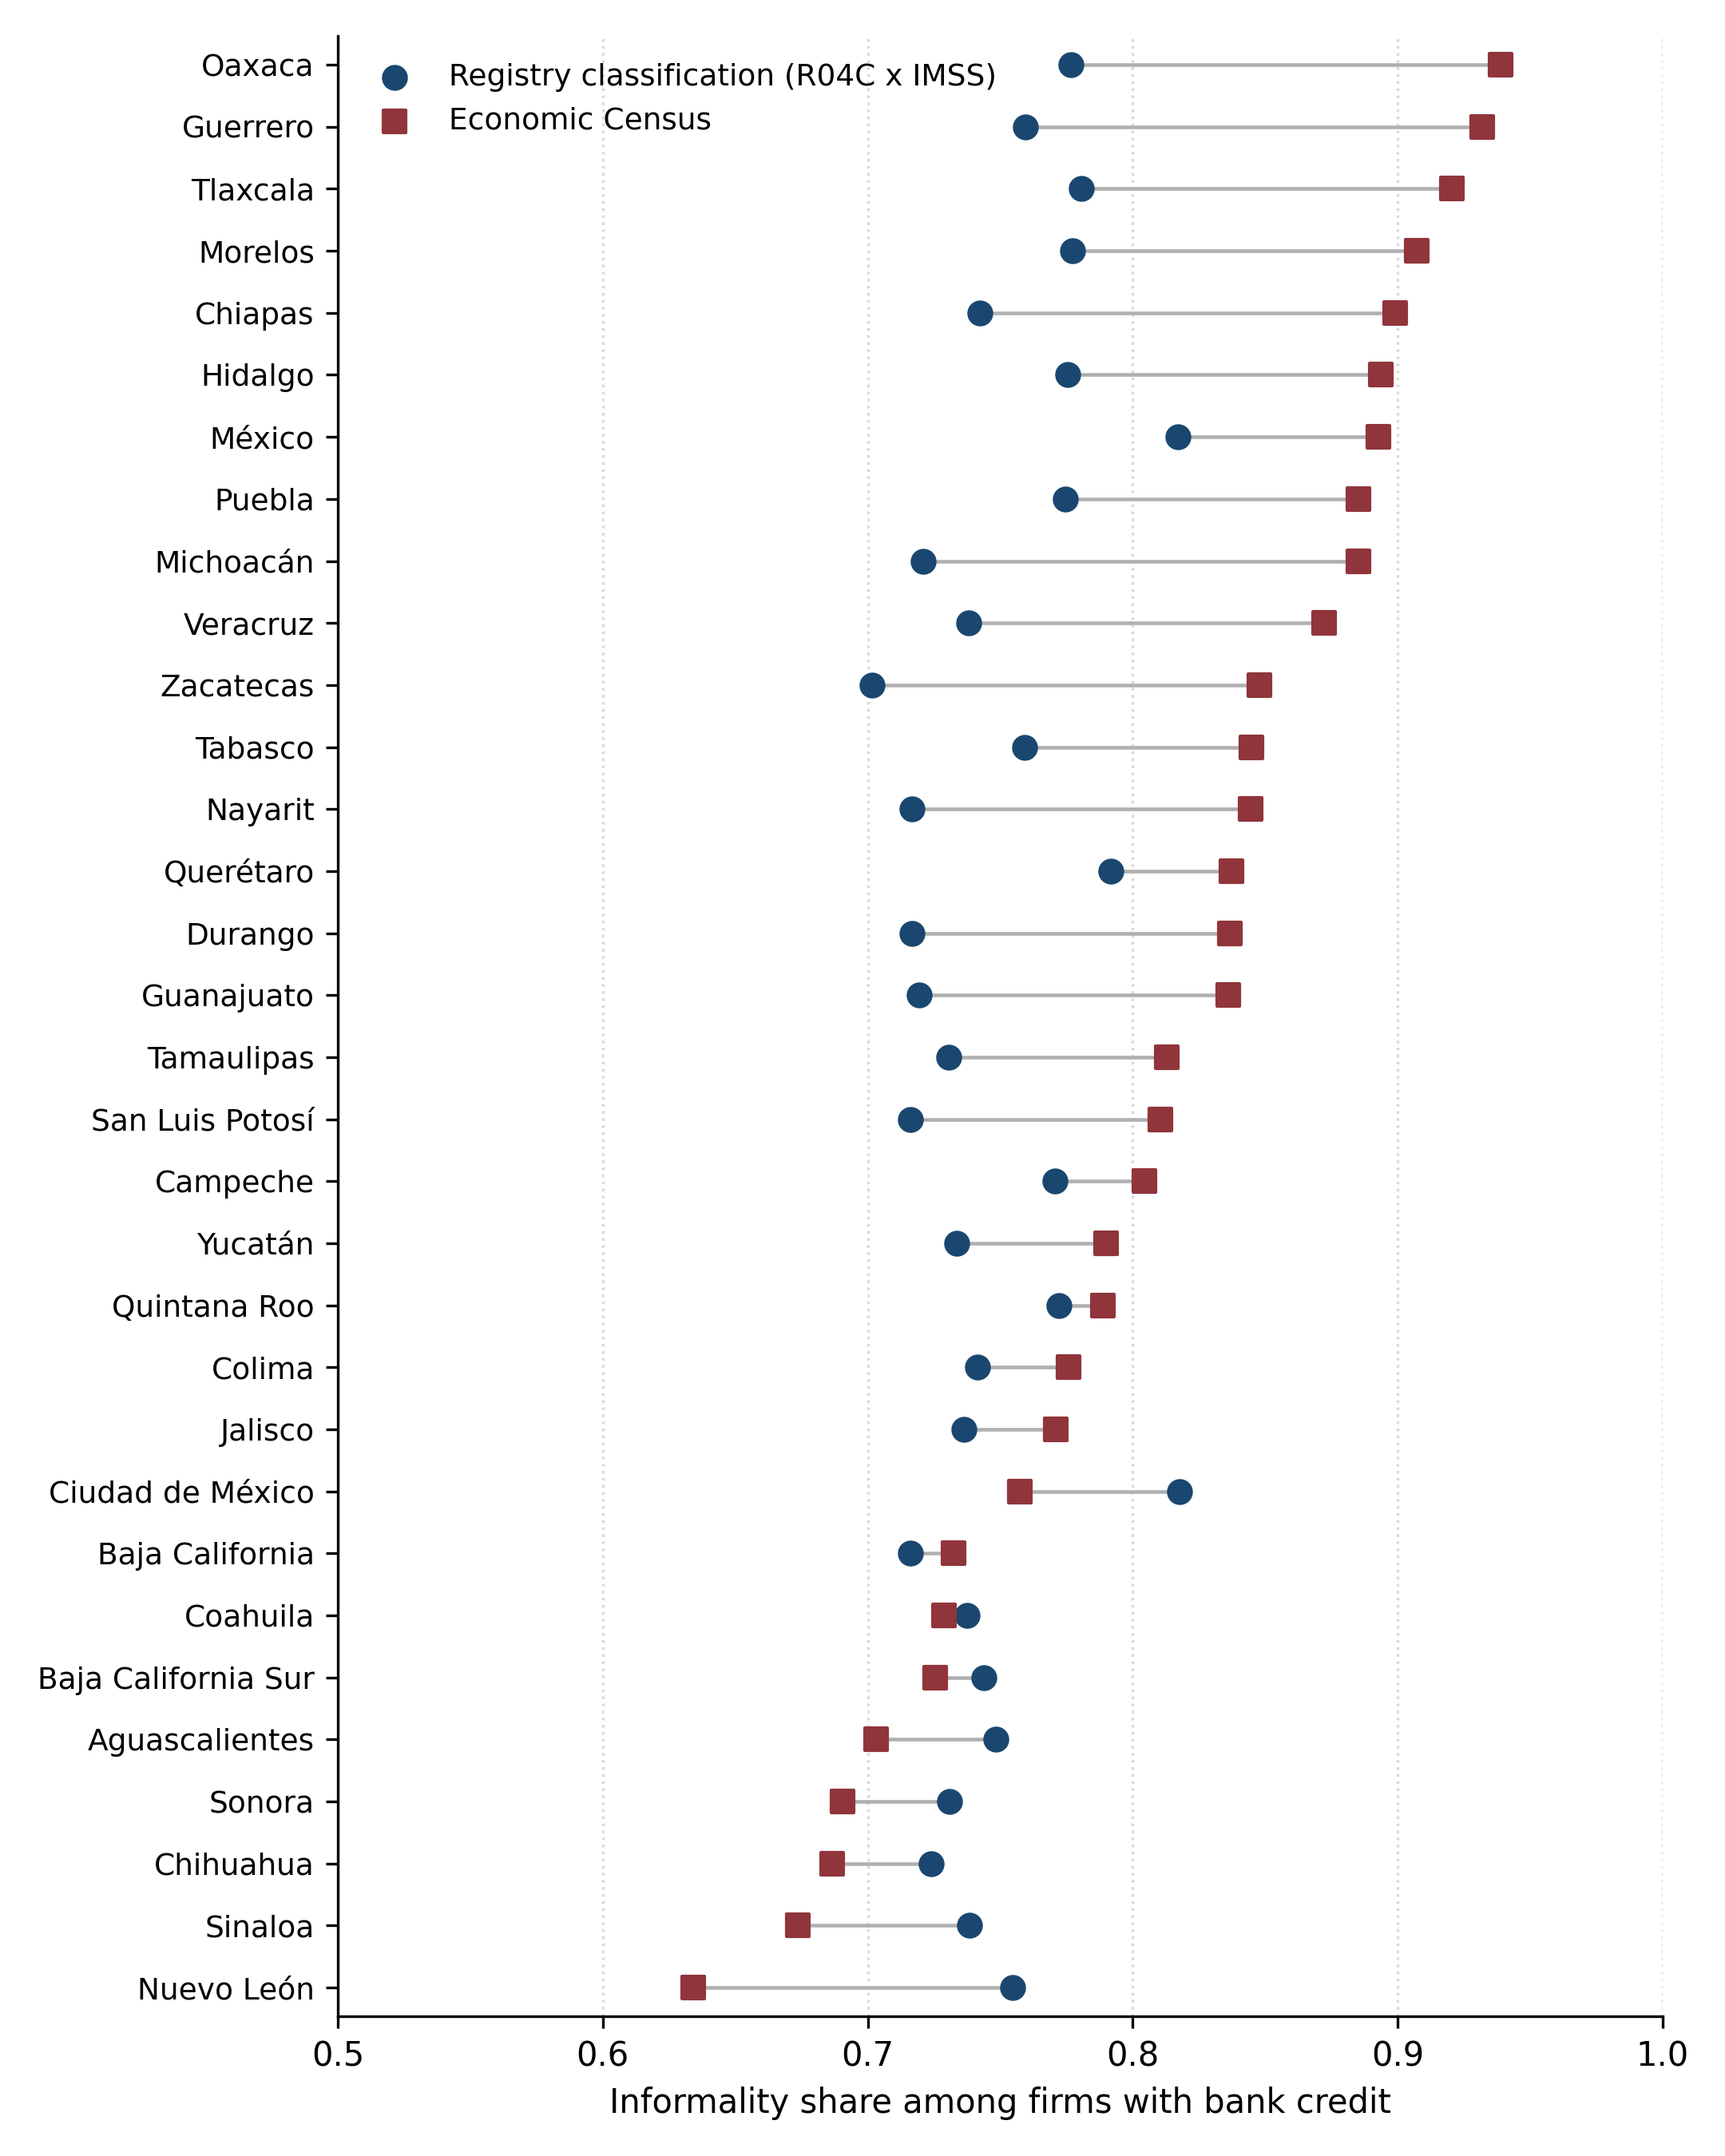
\includegraphics[width=0.8\textwidth]{slides_material/inf_valid_state.png}
    \par\footnotesize Share of firms with bank credit classified as informal, by state, sorted by the census value. Registry: firms borrowing in the 2018 R04C whose RFC has no IMSS employer registration (474{,}237 firms). Census: establishments not registered with IMSS (question h424a) among those reporting bank credit, 2019 census. The classification, used only for loan pricing, gets the level of borrower informality approximately right (76 percent overall against a census state mean of 81) but compresses the cross-state gradient: it overstates informality where the census puts it lowest (Nuevo Le\'on, Sinaloa, Chihuahua, Sonora) and understates it where the census puts it highest (Oaxaca, Guerrero, Tlaxcala, Morelos).
\end{figure}

\section{Census workers count} \label{workers_appendix_section}

\begin{table}[H] 
    \caption{Census worker counts}
    \label{workers_appendix}
    \centering
    \small
    \begin{threeparttable}
    \begin{tabular}{lccc}
        \toprule
        & Total & Formal & Informal \\
        \midrule
        $\widehat{\Delta_5\ln(\text{C})}$ & 0.037 & $-$0.071 & 0.074 \\
        & (0.082) & (0.193) & (0.204) \\
        \midrule
        FS Coeff. & $-$2.184 & $-$2.261 & $-$2.184 \\
                  & (1.589) & (1.454) & (1.589) \\
        FS F & 1.89 & 1.89 & 1.89 \\
        Obs. & 519 & 496 & 519 \\
        Markets & 519 & 496 & 519 \\
        \bottomrule
    \end{tabular}
    \begin{tablenotes}[flushleft]
        \footnotesize
        \item \textit{Notes:} Census worker counts exist only in the 2019 and 2024
        waves, leaving a single five-year window (a cross-section of markets, so
        clusters equal observations). The first stage on this subsample is weak
        (F $= 1.9$), so these estimates are reported for completeness only and are
        not informative. AKM standard errors in parentheses.
    \end{tablenotes}
\end{threeparttable}

\end{table}

% \section{Unweighted bank shocks statistics} \label{shock_stats_uw}

% \begin{table}[H] 
%     \caption{Unweighted moments of the standardized bank shocks}
%     \label{shock_stats_uw_table}
%     \centering
%     \small
%     \label{tab:bank_shocks_desc}
\begin{threeparttable}
\begin{tabular}{lcccccc}
\toprule
\textbf{Year} & Mean & Std. deviation & IQR \\
\midrule
2009 & -0.31 & 0.04 & 0.02 \\
2014 & -0.21 & 0.76 & 1.23 \\
2019 & 0.72 & 1.10 & 2.10 \\
2024 & -0.56 & 0.57 & 0.47 \\
\midrule
All & 0.00 & 1.00 & 0.98 \\
\bottomrule
\end{tabular}
\begin{tablenotes}[flushleft]
\item This table reports unweighted means, standard deviations, and
interquartile ranges of the standardized bank shocks $\hat{g}_{bt}^{std}$
across the four Economic Census waves, paralleling
Table~\ref{shock_stats}. Standardization is performed at the pooled
unweighted level so that the ``All'' row has mean $0$ and standard
deviation $1$ by construction. The effective sample size (ESS), largest
exposure, and No. banks are excluded from this table because they are the same as in table \ref{shock_stats}.
\end{tablenotes}
\end{threeparttable}
% \end{table}

\section{Additional descriptive statistics}
\label{app:descriptive_figs}

\begin{table}[H]
    \centering
    \caption{Estimation sample, census outcomes: establishments by formality and credit}
    \label{tab:desc_sample_census}
    \begin{threeparttable}
        \small
        \setlength{\tabcolsep}{5pt}
        \renewcommand{\arraystretch}{0.9}
        \begin{tabular}{l r r r r r r}
            \toprule
             & Mean & SD & p10 & Median & p90 & N \\
            \midrule
            \multicolumn{7}{l}{\textit{Panel A. Pooled levels at the start of the window, per market}} \\
            All firms & 8,874.6 & 29,241.7 & 415 & 2,319 & 20,316 & 1,394 \\
            \quad Formal & 1,094.3 & 3,872.7 & 13 & 138.5 & 2,695 & 1,394 \\
            \quad Informal & 7,780.3 & 25,628.2 & 393 & 2,159.5 & 17,436 & 1,394 \\
            Firms with bank credit & 572.8 & 1,793.1 & 3 & 119 & 1,331 & 1,394 \\
            \quad Formal & 136.6 & 547.7 & 0 & 12 & 280 & 1,394 \\
            \quad Informal & 436.2 & 1,277.0 & 1 & 95 & 1,035 & 1,394 \\
            Entrants & 4,139.1 & 12,961.3 & 164 & 984 & 9,540 & 996 \\
            \quad Formal & 449.9 & 1,672.9 & 5 & 50 & 973 & 996 \\
            \quad Informal & 3,689.1 & 11,400.7 & 156 & 923.5 & 8,454 & 996 \\
            Exits & 3,092.8 & 10,563.8 & 104 & 693 & 6,861 & 996 \\
            \quad Formal & 337.7 & 1,364.8 & 3 & 37 & 774 & 996 \\
            \quad Informal & 2,755.1 & 9,258.3 & 99 & 654.5 & 5,934 & 996 \\
            Switchers, informal to formal & 253.4 & 879.8 & 3 & 38.5 & 589 & 996 \\
            Switchers, formal to informal & 229.0 & 814.4 & 3 & 37 & 537 & 996 \\
            Stayers, formal & 390.0 & 1,427.8 & 2 & 42 & 938 & 996 \\
            Stayers, informal & 3,820.8 & 13,773.9 & 190 & 1,097 & 8,542 & 996 \\
            \addlinespace[3pt]
            \multicolumn{7}{l}{\textit{Panel B. Five year changes, log points}} \\
            All firms & 0.144 & 0.134 & 0.029 & 0.146 & 0.270 & 1,394 \\
            \quad Formal & 0.127 & 0.335 & $-$0.229 & 0.125 & 0.490 & 1,389 \\
            \quad Informal & 0.144 & 0.138 & 0.025 & 0.147 & 0.275 & 1,394 \\
            Firms with bank credit & 0.907 & 1.718 & $-$0.386 & 0.087 & 3.846 & 1,394 \\
            \quad Formal & 0.541 & 1.029 & $-$0.439 & 0.211 & 2.095 & 1,394 \\
            \quad Informal & 1.089 & 2.080 & $-$0.424 & 0.089 & 4.874 & 1,394 \\
            Entrants & 0.076 & 0.255 & $-$0.187 & 0.076 & 0.356 & 996 \\
            \quad Formal & $-$0.029 & 0.520 & $-$0.606 & $-$0.016 & 0.511 & 979 \\
            \quad Informal & 0.082 & 0.259 & $-$0.181 & 0.081 & 0.363 & 996 \\
            Exits & 0.036 & 0.256 & $-$0.211 & 0.044 & 0.300 & 996 \\
            \quad Formal & $-$0.051 & 0.543 & $-$0.693 & $-$0.045 & 0.655 & 965 \\
            \quad Informal & 0.040 & 0.264 & $-$0.211 & 0.046 & 0.306 & 996 \\
            Switchers, informal to formal & 0.050 & 0.589 & $-$0.693 & 0.061 & 0.690 & 957 \\
            Switchers, formal to informal & 0.228 & 0.584 & $-$0.434 & 0.222 & 0.916 & 958 \\
            Stayers, formal & 0.250 & 0.407 & $-$0.127 & 0.221 & 0.693 & 970 \\
            Stayers, informal & 0.203 & 0.158 & 0.075 & 0.196 & 0.346 & 996 \\
            \bottomrule
        \end{tabular}
        \begin{tablenotes}[flushleft]
            \footnotesize
            \item \textit{Notes:} The establishments from the Economic Censuses are aggregated to local labor markets. All statistics pool the 1,394 market window observations (556 markets, windows 2009-2014, 2014-2019, 2019-2024), unweighted. N smaller where undefined. Formal: positive number of workers and income with social security contributions. Entrants, exits, switchers and stayers are measured between consecutive censuses as in Table~\ref{firms_transition}.
        \end{tablenotes}
    \end{threeparttable}
\end{table}

\begin{table}[H]
    \centering
    \caption{Estimation sample, registry and social security records: outcomes and instrument}
    \label{tab:desc_sample_registry}
    \begin{threeparttable}
        \small
        \setlength{\tabcolsep}{5pt}
        \renewcommand{\arraystretch}{0.9}
        \begin{tabular}{l r r r r r r}
            \toprule
             & Mean & SD & p10 & Median & p90 & N \\
            \midrule
            \multicolumn{7}{l}{\textit{Panel A. Pooled levels at the start of the window, per market}} \\
            Borrowers & 556.8 & 3,714.0 & 4 & 50.5 & 919 & 1,394 \\
            \quad Formal & 107.9 & 623.2 & 0 & 7 & 177 & 1,394 \\
            \quad Informal & 448.9 & 3,151.9 & 3 & 39 & 747 & 1,394 \\
            Number of loans & 1,281.0 & 9,216.0 & 4 & 70 & 1,517 & 1,394 \\
            Total amount of authorized credit$^{\dagger}$ & 431.5 & 5,578.9 & 0.1 & 2.5 & 195.6 & 1,394 \\
            Average loan size$^{\ddagger}$ & 86.1 & 340.6 & 10.8 & 38.3 & 169.4 & 1,394 \\
            Loans per borrower & 2.27 & 26.64 & 1.00 & 1.38 & 2.22 & 1,394 \\
            Collateral ratio & 2.21 & 55.35 & 0.00 & 0.04 & 0.31 & 1,394 \\
            Interest rate (percent) & 14.86 & 4.56 & 8.88 & 14.91 & 20.30 & 1,394 \\
            Banks in the market & 10.1 & 9.0 & 2 & 7 & 21 & 1,394 \\
            IMSS workers & 26,655 & 142,866 & 37 & 1,316 & 47,088 & 1,394 \\
            IMSS wage bill, daily$^{\ddagger}$ & 415.2 & 2,706.8 & 0.3 & 12.8 & 546.2 & 1,394 \\
            \addlinespace[3pt]
            \multicolumn{7}{l}{\textit{Panel B. Five year changes, log points}} \\
            Borrowers & 0.298 & 0.888 & $-$0.676 & 0.295 & 1.424 & 1,394 \\
            \quad Formal & 0.558 & 0.830 & $-$0.340 & 0.693 & 1.542 & 1,130 \\
            \quad Informal & 0.211 & 0.928 & $-$0.807 & 0.182 & 1.409 & 1,379 \\
            Number of loans & 0.468 & 1.103 & $-$0.646 & 0.224 & 2.015 & 1,394 \\
            Total amount of authorized credit & 1.032 & 1.478 & $-$0.509 & 0.901 & 2.774 & 1,394 \\
            Average loan size & 0.565 & 1.045 & $-$0.459 & 0.520 & 1.663 & 1,394 \\
            Loans per borrower & 0.169 & 0.536 & $-$0.337 & 0.111 & 0.761 & 1,394 \\
            Collateral ratio & 0.702 & 2.455 & $-$1.600 & 0.597 & 3.128 & 820 \\
            Interest rate$^{\S}$ & 0.150 & 5.072 & $-$5.980 & 0.476 & 5.971 & 1,394 \\
            IMSS workers & 0.216 & 0.448 & $-$0.095 & 0.149 & 0.555 & 1,386 \\
            IMSS wage bill & 0.582 & 0.542 & 0.180 & 0.490 & 1.016 & 1,386 \\
            \addlinespace[3pt]
            \multicolumn{7}{l}{\textit{Panel C. Instrument}} \\
            Shift share instrument (standardized) & 0.248 & 1.197 & $-$0.893 & $-$0.261 & 2.063 & 1,394 \\
            Coverage & 0.921 & 0.110 & 0.762 & 0.967 & 1.000 & 1,394 \\
            \bottomrule
        \end{tabular}
        \begin{tablenotes}[flushleft]
            \footnotesize
            \item \textit{Notes:} Same sample and layout as Table~\ref{tab:desc_sample_census}. Credit registry, as delivered: borrowers are firms with a positive authorized line at a regulated bank in January, formal if IMSS employers that year. Loans are outstanding credit. Collateral ratio and interest rate are credit weighted market averages. Banks are the ones lending in that market. IMSS: workers and daily wage bill of IMSS employers in the market. $^{\dagger}$ million, $^{\ddagger}$ thousand dollars at 19 pesos per dollar. $^{\S}$ percentage points. Instrument standardized over all market windows with coverage. Coverage is the share of baseline credit held by banks with an estimated shock. 
        \end{tablenotes}
    \end{threeparttable}
\end{table}

\begin{table}[htbp]
    \centering
    \caption{Credit registry by year (January snapshot) and borrower status}
    \label{tab:desc_by_year}
    \begin{threeparttable}
        \small
        \setlength{\tabcolsep}{3.5pt}
        \renewcommand{\arraystretch}{0.9}
        \begin{tabular}{l r r r r r r r r r r}
            \toprule
             & \multicolumn{5}{c}{Formal borrowers} & \multicolumn{5}{c}{Informal borrowers} \\
            \cmidrule(lr){2-6} \cmidrule(lr){7-11}
            Year & N & Credit$^{\dagger}$ & Rate & No coll. & 2+ banks & N & Credit$^{\dagger}$ & Rate & No coll. & 2+ banks \\
            \midrule
            2005 & 2,516 & 31.6 & 16.00 & -- & 5.0 & 21,428 & 21.1 & 16.62 & -- & 2.0 \\
            2006 & 4,000 & 26.3 & 17.00 & -- & 6.3 & 33,379 & 15.8 & 18.18 & -- & 2.5 \\
            2007 & 5,717 & 21.1 & 16.30 & -- & 6.8 & 50,164 & 13.7 & 18.00 & -- & 3.0 \\
            2008 & 7,975 & 21.1 & 16.91 & -- & 8.1 & 73,658 & 13.7 & 19.31 & -- & 3.4 \\
            2009 & 9,568 & 18.8 & 18.10 & -- & 8.7 & 78,573 & 13.2 & 19.50 & -- & 3.8 \\
            2010 & 25,513 & 26.3 & 13.93 & 74.6 & 28.9 & 226,512 & 10.5 & 14.95 & 89.7 & 12.8 \\
            2011 & 28,888 & 26.3 & 14.07 & 75.4 & 29.3 & 228,728 & 10.9 & 15.38 & 88.9 & 13.0 \\
            2012 & 32,797 & 26.3 & 14.46 & 74.7 & 29.7 & 239,564 & 11.1 & 15.80 & 87.9 & 13.6 \\
            2013 & 38,581 & 26.3 & 14.79 & 77.4 & 28.3 & 259,762 & 11.6 & 16.24 & 88.9 & 14.0 \\
            2014 & 42,355 & 29.5 & 13.76 & 77.6 & 28.0 & 252,567 & 11.6 & 15.17 & 87.9 & 14.3 \\
            2015 & 46,402 & 32.6 & 13.24 & 80.6 & 27.8 & 252,332 & 12.8 & 14.59 & 88.9 & 14.3 \\
            2016 & 53,007 & 34.6 & 13.06 & 82.3 & 26.9 & 249,152 & 13.2 & 14.54 & 88.5 & 14.3 \\
            2017 & 80,833 & 48.5 & 16.00 & 79.6 & 21.3 & 279,487 & 15.2 & 17.55 & 83.7 & 7.5 \\
            2018 & 94,356 & 43.7 & 16.58 & 85.2 & 23.8 & 310,486 & 15.3 & 17.63 & 89.9 & 8.1 \\
            2019 & 99,452 & 46.7 & 17.21 & 81.8 & 23.7 & 299,635 & 15.7 & 18.34 & 88.2 & 8.2 \\
            2020 & 96,694 & 52.4 & 17.00 & 78.0 & 22.3 & 282,031 & 14.8 & 18.14 & 86.7 & 7.2 \\
            2021 & 90,647 & 52.6 & 14.96 & 76.8 & 21.2 & 246,308 & 15.8 & 15.85 & 86.0 & 6.8 \\
            2022 & 86,710 & 54.3 & 14.71 & 76.3 & 22.7 & 256,537 & 14.5 & 15.29 & 89.2 & 7.0 \\
            2023 & 77,402 & 67.1 & 15.69 & 92.0 & 23.3 & 154,974 & 22.1 & 15.69 & 92.6 & 9.9 \\
            2024 & 83,334 & 74.7 & 16.45 & 79.4 & 24.1 & 171,635 & 22.7 & 16.65 & 85.6 & 10.3 \\
            2025 & 83,187 & 84.2 & 16.20 & -- & 25.8 & 165,867 & 26.6 & 15.95 & -- & 12.4 \\
            \bottomrule
        \end{tabular}
        \begin{tablenotes}[flushleft]
            \footnotesize
            \item \textit{Notes:} Credit registry matched to IMSS employer records. A borrower is formal in a given year if it appears as an IMSS employer that year. Borrowers: firms with a positive authorized line. Credit: median borrower authorized credit, $^{\dagger}$in nominal thousand dollars, at 19 pesos per dollar. Rate: median annualized gross rate at the bank relationship level, percent, winsorized at the 1st and 99th percentiles within year. No coll.: share of relationships without collateral, percent, reported for the years in which the registry carries the collateral field. 2+ banks: share of borrowers with two or more banks, percent. 
            %The number of borrowers reported rises steeply until 2010 as the registry's reporting of commercial loans expands; the breaks in 2017 and 2023 coincide with changes in the reporting layout and are under review with the data provider (Appendix~\ref{app:data})."
        \end{tablenotes}
    \end{threeparttable}
\end{table}

\begin{table}[H]
    \centering
    \caption{Estimation sample and all market windows with an instrument}
    \label{tab:desc_sample_all}
    \begin{threeparttable}
        \small
        \setlength{\tabcolsep}{3.5pt}
        \renewcommand{\arraystretch}{0.9}
        \begin{tabular}{l r r r r r r r r r}
            \toprule
             & \multicolumn{3}{c}{All market windows} & \multicolumn{6}{c}{Estimation sample, by window} \\
            \cmidrule(lr){2-4} \cmidrule(lr){5-10}
             & & & & \multicolumn{2}{c}{2009-2014} & \multicolumn{2}{c}{2014-2019} & \multicolumn{2}{c}{2019-2024} \\
            \cmidrule(lr){5-6} \cmidrule(lr){7-8} \cmidrule(lr){9-10}
             & Mean & Median & N & Mean & Median & Mean & Median & Mean & Median \\
            \midrule
            \multicolumn{10}{l}{\textit{Panel A. Pooled levels at the start of the window, per market}} \\
            All firms & 7,244.4 & 1,699 & 1,748 & 8,980.7 & 2,675 & 8,564.4 & 2,113 & 9,078.4 & 2,271 \\
            \quad Formal & 882.9 & 88 & 1,748 & 1,096.9 & 159 & 1,072.9 & 139 & 1,112.1 & 120 \\
            \quad Informal & 6,361.6 & 1,605.5 & 1,748 & 7,883.8 & 2,453.5 & 7,491.4 & 1,989 & 7,966.3 & 2,128 \\
            With a loan (census) & 465.5 & 73 & 1,748 & 98.4 & 10.5 & 787.6 & 208 & 739.1 & 199 \\
            Informal$\to$Formal & 212.4 & 25 & 1,204 & - & - & 236.1 & 44 & 269.2 & 34 \\
            Formal$\to$Informal & 191.9 & 23 & 1,204 & - & - & 207.7 & 30 & 248.5 & 42 \\
            Borrowers (registry) & 470.5 & 33 & 1,662 & 218.7 & 28 & 610.9 & 58 & 766.4 & 66 \\
            Total credit$^{\dagger}$ & 345.3 & 1.3 & 1,748 & 28.9 & 0.7 & 663.2 & 2.2 & 526.3 & 6.0 \\
            Collateral ratio & 1.87 & 0.03 & 1,662 & - & - & 0.11 & 0.09 & 5.84 & 0.10 \\
            Interest rate (\%) & 15.01 & 14.91 & 1,662 & 15.89 & 15.87 & 12.36 & 12.57 & 16.36 & 16.25 \\
            IMSS workers & 22,360 & 837 & 1,674 & 25,687 & 1,642 & 25,289 & 1,195 & 28,654 & 1,168 \\
            \addlinespace[3pt]
            \multicolumn{10}{l}{\textit{Panel B. Instrument}} \\
            Shift share IV (std.) & 0.000 & $-$0.449 & 2,356 & $-$0.225 & $-$0.211 & 1.788 & 1.927 & $-$0.804 & $-$0.809 \\
            Coverage & 0.702 & 0.938 & 2,356 & 0.937 & 0.991 & 0.925 & 0.975 & 0.905 & 0.945 \\
            \bottomrule
        \end{tabular}
        \begin{tablenotes}[flushleft]
            \footnotesize
            \item \textit{Notes:} First three columns include every market window for which the instrument is defined, unweighted, N per row (Panel B includes three windows, panel A includes two windows since there is no 2004 information). Last six columns are the estimation sample of the Table`\ref{tab:desc_sample} by window, with 398, 477 and 519 markets per window, respectively. Switchers (F$\to$I and I$\to$F) are undefined for the 2009 baseline. Variables and sources as in that table. $^{\dagger}$ Million dollars at 19 pesos per dollar.
        \end{tablenotes}
    \end{threeparttable}
\end{table}

\begin{figure}[H]
    \caption{Capital, investment, and debt by formality}
    \label{fig:enafin_gaps}
    \centering
    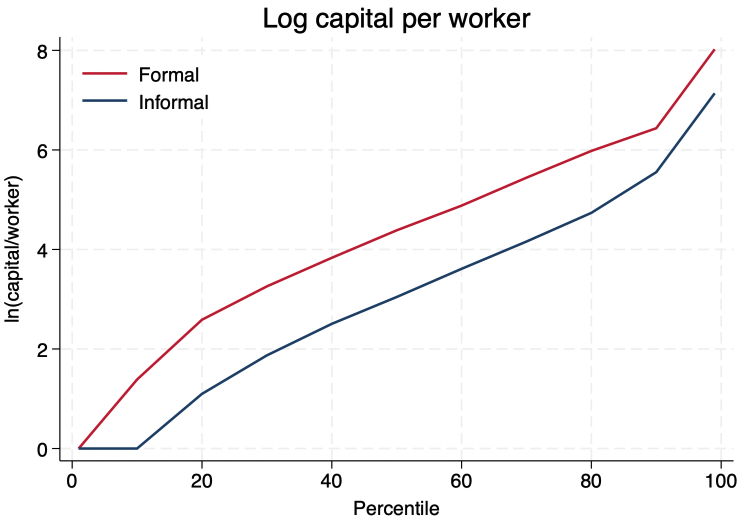
\includegraphics[width=0.48\textwidth]{slides_material/l_k_w.png}
    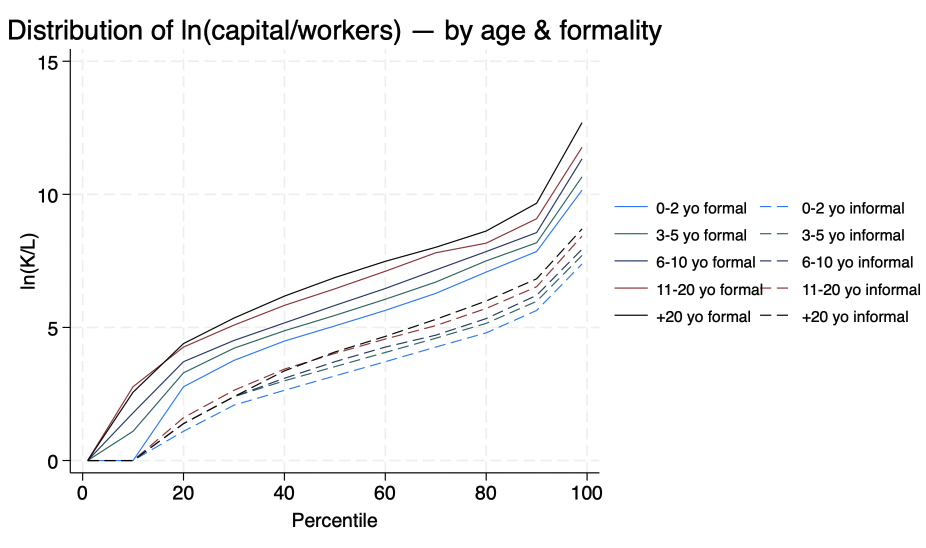
\includegraphics[width=0.48\textwidth]{slides_material/l_k_w_age.png}\\[2mm]
    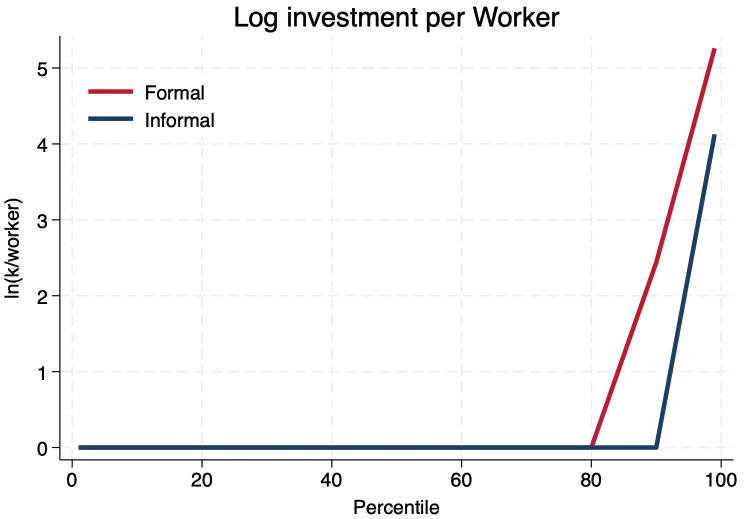
\includegraphics[width=0.48\textwidth]{slides_material/l_i_w.png}
    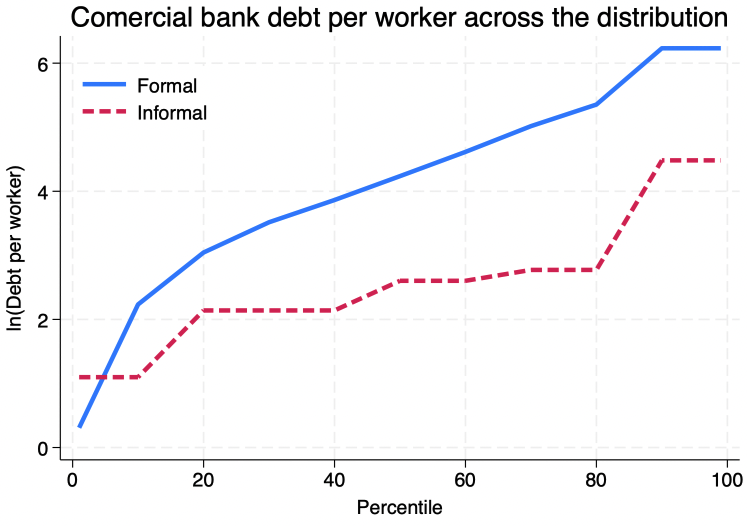
\includegraphics[width=0.48\textwidth]{slides_material/debt_w.png}
    \par\footnotesize Census capital per worker by size and by age, census investment per worker, and survey bank debt per worker, formal against informal firms.
\end{figure}

% \begin{figure}[H]
%     \caption{Informality and credit across countries}
%     \label{fig:crosscountry}
%     \centering
%     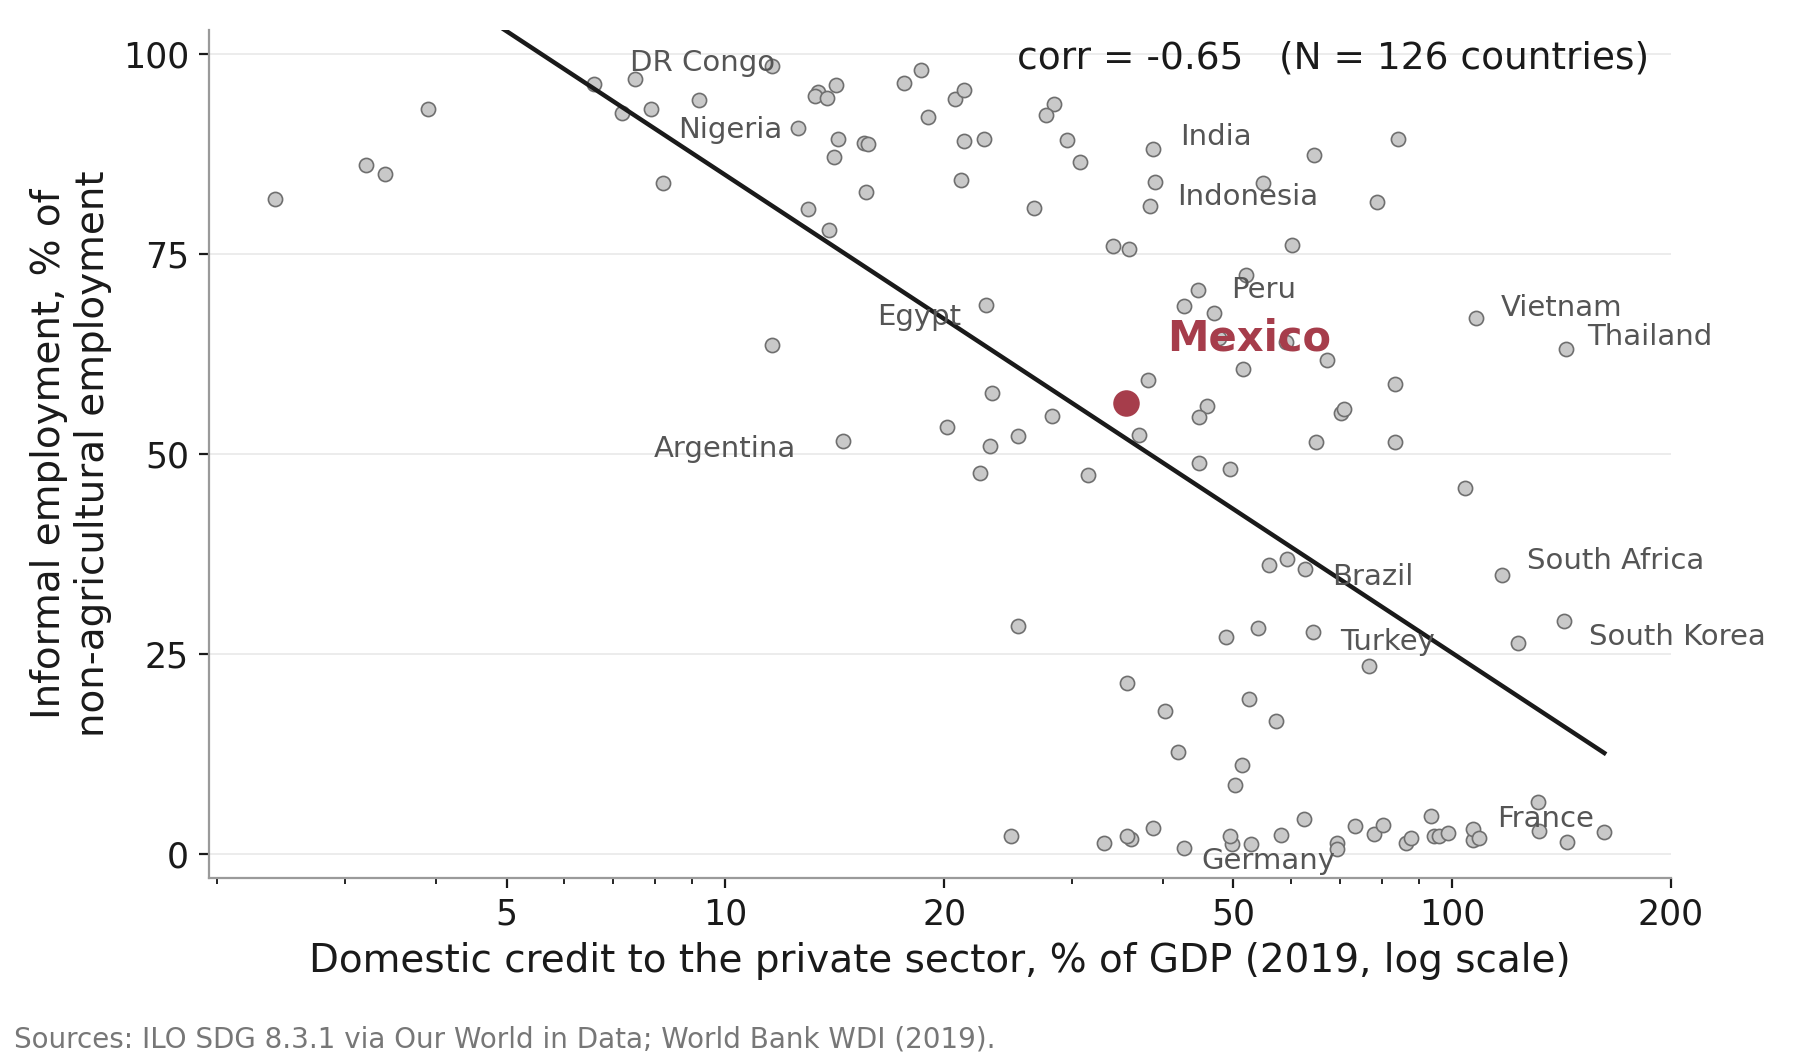
\includegraphics[width=0.75\textwidth]{slides_material/fig_crosscountry_informality.png}
% \end{figure}

\section{Within-firm validation of the bank credit supply shocks} \label{firm_km_section}

\begin{table}[H]
    \caption{Firm-level responses to bank credit supply shocks}
    \label{firm_km_table}
    \centering
    \small
    \begin{threeparttable}
    \begin{tabular}{@{}lrrr@{}}
        \toprule
         & Coefficient (s.e.) & Mean & $N$ \\
        \midrule
        Within-firm credit growth on bank shock$^{\dagger}$ & 0.131\sym{***} (0.021) & 0.038 & 1,020,447 \\
        \quad weighted by lagged credit & 0.454\sym{***} (0.052) & $-$0.425 & 1,020,447 \\
        Firm credit growth on its banks' shocks & 0.016\sym{***} (0.004) & 0.035 & 3,704,022 \\
        \quad two or more banks & 0.092\sym{***} (0.013) & 0.067 & 430,148 \\
        \quad single bank & 0.011\sym{***} (0.004) & 0.030 & 3,272,491 \\
        \bottomrule
    \end{tabular}
    \begin{tablenotes}[flushleft]
        \footnotesize
        \item Khwaja and Mian (2008) estimates on the annual firm-bank panel. Rows 1 and 2: log credit growth of a firm-bank pair on the bank's credit supply shock (log points), with firm-by-year fixed effects, among firms with two or more banks. The second row weights pairs by lagged credit. Rows 3 to 5: a firm's log credit growth on the standardized lagged-share-weighted average of its banks' shocks, with market-by-year fixed effects, among firm-years whose banks with a shock hold at least half of its lagged credit. Standard errors clustered by market. $^{\dagger}$Clustered by bank, the standard error is 0.045. Means of the dependent variable in each sample, weighted where the regression is. $N$: firm-bank-years in rows 1 and 2, firm-years in rows 3 to 5. Rates winsorized at 1 and 99 percent by year (Appendix~\ref{app:data}). \sym{*}~$p<0.10$, \sym{**}~$p<0.05$, \sym{***}~$p<0.01$.
    \end{tablenotes}
\end{threeparttable}

\end{table}


\section{Map of credit growth} \label{credit_growth}

\begin{figure}[H]
    \caption{Five year credit growth across markets}
    \label{fig:map_credit}
    \centering
    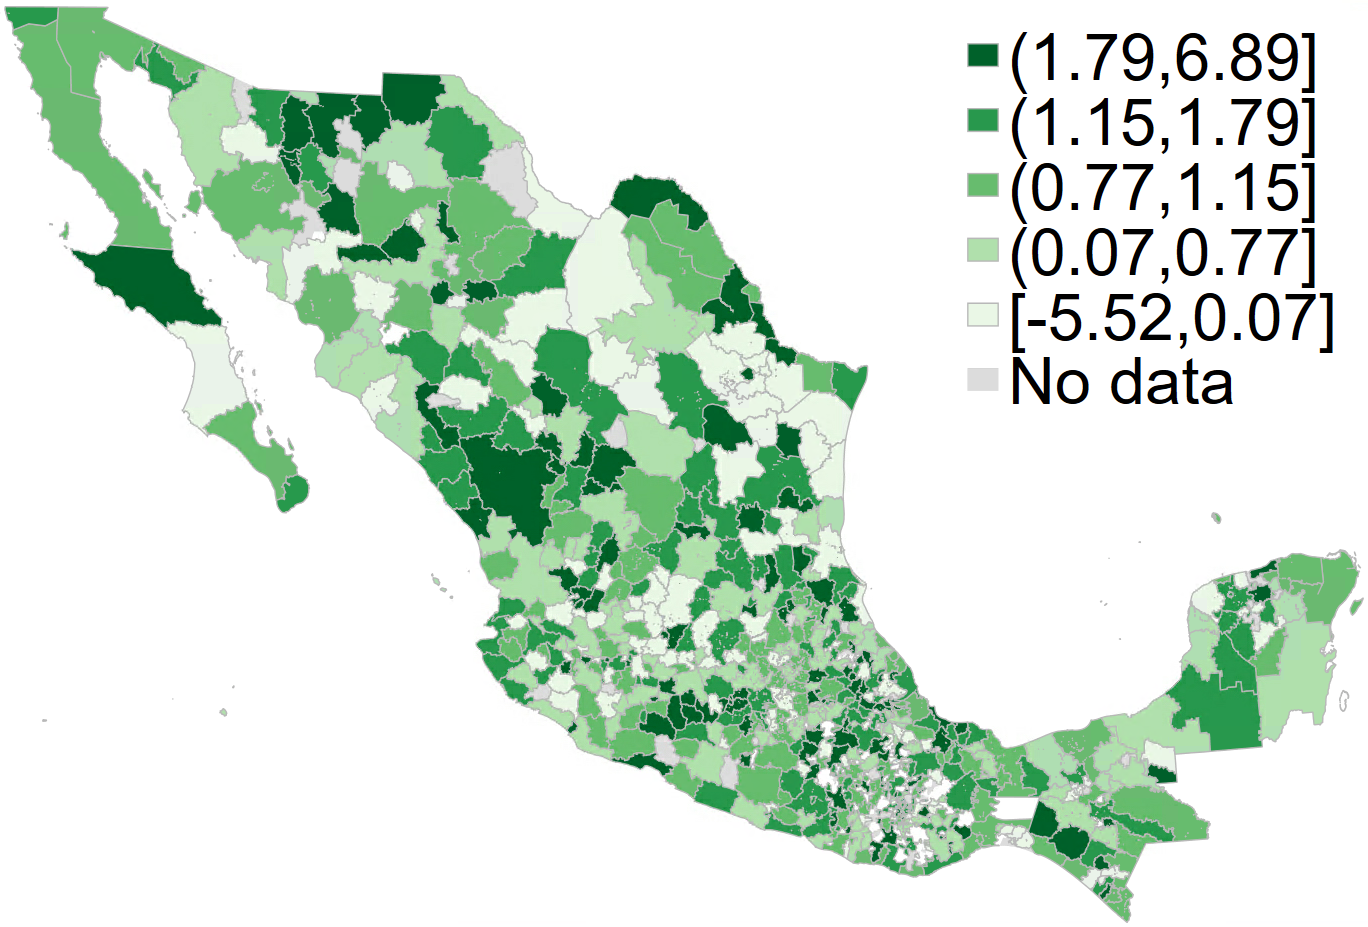
\includegraphics[width=0.6\textwidth]{slides_material/map_credit.png}
    \par\footnotesize Realized five year log change in bank credit by local labor market, the outcome side of the first stage.
\end{figure}

\section{Annual shift-Share IV estimates} \label{annual_appendix}

\begin{table}[H]
    \caption{Annual event study coefficients by horizon}
    \label{annual_table}
    \centering
    \small
    \begin{threeparttable}
\caption{Annual event study coefficients by horizon}
\label{tab:event_horizons}
\begin{tabular}{@{}crrrrrrr@{}}
\toprule
 & & \multicolumn{2}{c}{Credit} & \multicolumn{2}{c}{Interest rate (pp)} & \multicolumn{2}{c}{Collateral ratio} \\
\cmidrule(lr){3-4} \cmidrule(lr){5-6} \cmidrule(lr){7-8}
$h$ & Credit & Formal & Informal & Formal & Informal & Formal & Informal \\
\midrule
$-4$ & $-$0.082\sym{**} & $-$0.097\sym{*} & $-$0.077 & 0.168 & $-$0.046 & 0.151\sym{***} & 0.071\sym{*} \\
 & (0.041) & (0.056) & (0.049) & (0.111) & (0.098) & (0.050) & (0.040) \\
$-3$ & 0.004 & $-$0.039 & 0.016 & $-$0.013 & 0.118\sym{**} & 0.090 & 0.074 \\
 & (0.027) & (0.024) & (0.026) & (0.042) & (0.052) & (0.058) & (0.045) \\
$-2$ & $-$0.127\sym{***} & $-$0.064 & $-$0.132\sym{***} & 0.185\sym{**} & $-$0.080 & $-$0.031 & 0.101\sym{***} \\
 & (0.033) & (0.049) & (0.041) & (0.089) & (0.069) & (0.059) & (0.037) \\
$-1$ & $-$0.043 & $-$0.054 & $-$0.006 & $-$0.064 & $-$0.103\sym{***} & 0.021 & 0.021 \\
 & (0.027) & (0.072) & (0.055) & (0.075) & (0.035) & (0.060) & (0.053) \\
$0$ & 0.140\sym{***} & 0.192\sym{***} & 0.076\sym{***} & $-$0.274\sym{***} & $-$0.021 & $-$0.075 & $-$0.075 \\
 & (0.031) & (0.043) & (0.030) & (0.096) & (0.110) & (0.131) & (0.084) \\
$1$ & 0.128\sym{***} & 0.200\sym{***} & 0.057 & $-$0.172\sym{**} & 0.118\sym{*} & $-$0.267\sym{***} & $-$0.158 \\
 & (0.033) & (0.035) & (0.037) & (0.087) & (0.066) & (0.076) & (0.115) \\
$2$ & 0.220\sym{***} & 0.223\sym{***} & 0.158\sym{**} & $-$0.262\sym{***} & 0.073 & $-$0.208\sym{*} & $-$0.193\sym{***} \\
 & (0.053) & (0.044) & (0.065) & (0.083) & (0.060) & (0.115) & (0.071) \\
$3$ & 0.227\sym{***} & 0.215\sym{***} & 0.162\sym{***} & $-$0.133 & 0.029 & $-$0.238\sym{**} & $-$0.198\sym{***} \\
 & (0.051) & (0.044) & (0.061) & (0.129) & (0.066) & (0.118) & (0.068) \\
$4$ & 0.201\sym{***} & 0.176\sym{***} & 0.146\sym{**} & $-$0.519\sym{***} & $-$0.120 & $-$0.289\sym{**} & $-$0.138 \\
 & (0.052) & (0.044) & (0.066) & (0.130) & (0.121) & (0.124) & (0.089) \\
\bottomrule
\end{tabular}
\begin{tablenotes}[flushleft]
\footnotesize
\item Coefficients plotted in Figures~\ref{fig:event_credit}, \ref{fig:event_credit_fmlty}, \ref{fig:event_r_fmlty} and \ref{fig:event_col_fmlty}: reduced-form estimates on the annual market panel of the outcome $h$ years after the shock on the IV, one regression per horizon and column, with the annual analogs of the main specification's controls, weighted by the market's lagged credit, on market-years with instrument coverage of at least $0.5$. Standard errors clustered by market in parentheses. Stars from the corresponding two-sided tests. Credit columns in logs, interest rates in percentage points, the collateral ratio in logs. Market-years per regression range from 7,697 to 10,002 in the credit column, 5,859 to 7,840 in the formal credit and rate columns, 7,622 to 9,915 in the informal ones, 2,805 to 4,314 and 3,780 to 5,689 in the formal and informal collateral columns. \sym{*}~$p<0.10$, \sym{**}~$p<0.05$, \sym{***}~$p<0.01$.
\end{tablenotes}
\end{threeparttable}

\end{table}

\begin{table}[H]
    \caption{Annual event study coefficients by horizon: additional outcomes}
    \label{annual_table2}
    \centering
    \small
    \begin{threeparttable}
\footnotesize
\setlength{\tabcolsep}{3pt}
\begin{tabular}{@{}lrrrrrrrrr@{}}
\toprule
 & \multicolumn{9}{c}{Years since shock, $h$} \\
\cmidrule(lr){2-10}
 & $-4$ & $-3$ & $-2$ & $-1$ & $0$ & $1$ & $2$ & $3$ & $4$ \\
\midrule
\multicolumn{10}{@{}l}{\textit{Number of loans (log)}} \\
\quad Formal & 0.36 & 1.45 & $-$3.41 & $-$1.65\sym{*} & $-$0.80 & $-$0.73 & $-$0.07 & 0.01 & 0.52 \\
 & (0.82) & (1.18) & (2.50) & (0.95) & (0.83) & (0.96) & (0.99) & (1.00) & (1.04) \\
\quad Informal & 0.52 & 1.91 & $-$4.18 & $-$2.07 & $-$3.22\sym{*} & $-$3.28 & $-$0.62 & $-$0.12 & 0.06 \\
 & (1.00) & (1.54) & (2.73) & (1.38) & (1.95) & (2.07) & (3.26) & (2.81) & (3.27) \\
\addlinespace[3pt]
\multicolumn{10}{@{}l}{\textit{Number of borrowers (log)}} \\
\quad Formal & 0.11 & 1.25 & $-$3.26 & $-$1.66\sym{*} & $-$0.69 & $-$0.93 & $-$0.49 & $-$0.31 & 0.17 \\
 & (0.87) & (1.10) & (2.50) & (0.98) & (0.74) & (0.81) & (0.82) & (0.82) & (0.88) \\
\quad Informal & 0.41 & 1.86 & $-$4.20 & $-$2.00 & $-$3.23\sym{*} & $-$3.22 & $-$0.88 & $-$0.50 & $-$0.33 \\
 & (1.02) & (1.52) & (2.70) & (1.44) & (1.87) & (1.97) & (3.10) & (2.61) & (3.07) \\
\addlinespace[3pt]
\multicolumn{10}{@{}l}{\textit{Loans per borrower (log)}} \\
\quad Formal & $-$0.25 & 0.20 & $-$0.15 & 0.02 & $-$0.10 & 0.20 & 0.42\sym{*} & 0.31 & 0.35 \\
 & (0.18) & (0.17) & (0.10) & (0.14) & (0.18) & (0.22) & (0.25) & (0.26) & (0.30) \\
\quad Informal & 0.12 & 0.05 & 0.02 & $-$0.07 & 0.02 & $-$0.05 & 0.26 & 0.38 & 0.39 \\
 & (0.09) & (0.10) & (0.08) & (0.09) & (0.13) & (0.17) & (0.20) & (0.24) & (0.25) \\
\addlinespace[3pt]
\multicolumn{10}{@{}l}{\textit{Credit per loan (log)}} \\
\quad Formal & $-$10.06\sym{*} & $-$5.31\sym{**} & $-$3.03 & $-$3.79 & 19.96\sym{***} & 20.74\sym{***} & 22.35\sym{***} & 21.48\sym{***} & 17.07\sym{***} \\
 & (5.58) & (2.55) & (4.84) & (7.70) & (3.74) & (2.85) & (3.88) & (3.80) & (3.70) \\
\quad Informal & $-$8.25\sym{*} & $-$0.28 & $-$8.99\sym{***} & 1.44 & 10.86\sym{***} & 8.98\sym{***} & 16.38\sym{***} & 16.29\sym{***} & 14.53\sym{***} \\
 & (4.47) & (2.42) & (2.98) & (5.03) & (2.95) & (3.40) & (4.75) & (4.84) & (5.37) \\
\addlinespace[3pt]
\multicolumn{10}{@{}l}{\textit{Share of loans without collateral}} \\
\quad Formal & $-$0.06 & 0.13 & $-$0.20 & 0.07 & $-$0.79\sym{***} & $-$0.50 & $-$0.83\sym{***} & $-$0.70\sym{**} & $-$0.76\sym{**} \\
 & (0.10) & (0.19) & (0.13) & (0.14) & (0.30) & (0.30) & (0.30) & (0.33) & (0.34) \\
\quad Informal & $-$0.14\sym{**} & 0.14 & $-$0.05 & 0.07 & $-$0.58\sym{**} & $-$0.18 & $-$0.38\sym{***} & $-$0.26 & $-$0.36\sym{*} \\
 & (0.07) & (0.12) & (0.06) & (0.07) & (0.23) & (0.17) & (0.14) & (0.17) & (0.20) \\
\addlinespace[3pt]
\multicolumn{10}{@{}l}{\textit{Formal sector, IMSS (log)}} \\
\quad Employment & 0.19 & 0.33\sym{*} & 0.25 & $-$0.07 & 0.10 & 0.09 & 0.53\sym{*} & 0.59\sym{*} & 0.22 \\
 & (0.16) & (0.19) & (0.16) & (0.17) & (0.18) & (0.21) & (0.32) & (0.32) & (0.43) \\
\quad Mean wage & 0.22\sym{**} & 0.24\sym{**} & 0.06 & 0.22\sym{***} & 0.01 & $-$0.02 & 0.16 & 0.16 & 0.04 \\
 & (0.09) & (0.12) & (0.11) & (0.07) & (0.08) & (0.16) & (0.17) & (0.20) & (0.22) \\
\bottomrule
\end{tabular}
\begin{tablenotes}[flushleft]
\footnotesize
\item Same specification as Table~\ref{tab:event_horizons}, one regression per horizon and row. Coefficients and standard errors are multiplied by 100, so log outcomes read as percent and the share of loans without collateral in percentage points. Loans, borrowers, loans per borrower and credit per loan are market totals or ratios for loans to formal and to informal borrowers. The share without collateral is the share of loans with no posted collateral. Employment and mean wage are the market's IMSS registered workers and their mean wage. Standard errors clustered by market in parentheses. Market years per regression range from 5,859 to 7,840 for the formal borrower series, 7,622 to 9,915 for the informal ones and 7,738 to 9,969 for employment and wages. \sym{*}~$p<0.10$, \sym{**}~$p<0.05$, \sym{***}~$p<0.01$.
\end{tablenotes}
\end{threeparttable}
\end{table}

\section{Robustness checks} \label{robustness_appendix}

This appendix examines the robustness of the five-year results. We proceed in three steps. First, we test the identifying assumption directly. We check that the exposure shares are balanced on predetermined market characteristics, we control for lagged outcome changes, and we run placebo regressions on pre-period outcomes. Second, we vary the construction of the instrument. We drop the Leave-One-Out correction, renormalize by coverage, move the coverage threshold from zero to $0.8$, and rebuild the instrument without the largest lender. Third, we vary the population and the estimator. We exclude the three metropolitan areas, drop the credit weights, compare the IV estimates with their OLS and reduced-form counterparts, and re-estimate everything at the bank level with re-identified shocks. The corresponding tables follow. One result survives every exercise: credit supply shifts the composition of firms toward formality without changing their number.

A central identifying assumption of our design is that the bank credit supply shocks aggregated by the Shift-Share instrument are as-good-as-randomly assigned conditional on the controls in our main specification. Following the balance tests suggested by \citet{borusyak2022quasi} and \citet{goldsmith2020bartik}, we regress each of the seven predetermined market controls of the main specification on the Leave-One-Out Shift-Share instrument, conditional on year fixed effects and the coverage control and weighted by baseline market credit. Table~\ref{balance_test_table} reports the results with each control measured five and ten years before the baseline period, that is, ten and fifteen years before the outcome wave. None of the fourteen coefficients is statistically distinguishable from zero at the ten percent level (the smallest $p$-value is $0.12$) and the point estimates are economically small. As a complementary dynamic check, Table~\ref{pretrend_test_table} re-estimates the main specifications adding the dependent variable's own lagged five-year change as a control. The core results are essentially unchanged, with the formal-firm response at $0.048$ against $0.050$ in the baseline; the exceptions are the aggregate and formal value-added responses, which reverse sign under this control and on which we therefore do not lean, while the value-added result we emphasize, the reallocation of production away from the informal sector, strengthens under it.

As a model-free check on our identification, Table~\ref{reduced_form_table} reports, for every outcome, the naive OLS regression on credit growth and the reduced-form regression on the standardized Leave-One-Out instrument, with the same controls, weights, and sample restrictions as the main IV specification and standard errors clustered at the market level. The reduced form confirms that the identifying correlation is present in the raw data, with significance concentrated in the same margins the paper emphasizes (formal firms $0.056$, s.e.\ $0.016$; formal entry $0.075$; informal exit $0.062$), and the OLS-IV comparison shows why instrumenting matters: OLS is attenuated relative to IV on the composition margins (the formal stock at $0.025$ against $0.050$, formalization at $0.031$ against $0.052$), the pattern expected when demand shocks dominate observational credit variation.

The credit-weighted regression places disproportionate weight on the three largest metropolitan areas (Mexico City, Monterrey, and Guadalajara). To address the concern that the main estimates reflect dynamics specific to these urban banking centers, Table~\ref{iv_nometros_table} re-estimates every specification excluding them, nine of the 1,394 market-year observations. The composition core is essentially unchanged, with the formal-firm response at $0.049$ against $0.050$ and formal entry identical at $0.067$, and several margins strengthen outside the metros (the employment response rises to $0.028$ and the informal value-added decline deepens to $-0.115$). Two results soften and are disclosed as such: the informal-to-formal switching flow loses significance, with the composition shift operating instead through formal retention ($0.055$), fewer switches into informality ($-0.049$), and a declining count of informal stayers ($-0.025$), and the mean-wage decline disappears, indicating that the wage-composition effect of marginal hires is a metropolitan phenomenon. Dropping the largest markets therefore leaves the formalization core intact.

The credit weights in our main specification imply that the elasticities in Tables~\ref{main_table}--\ref{main_econ_table} are credit-weighted averages of market-specific responses, in which markets with larger base-period credit, notably the three metropolitan areas, carry proportionally more weight. Table~\ref{unweighted_table} therefore re-estimates the main specification with every market-year contributing equally, which shifts the estimand toward the typical market, a market with roughly \$2.5 million (USD) of credit outstanding at baseline, on estimation samples identical to the weighted ones. The first stage remains adequate (Kleibergen--Paap $F$ between $27$ and $54$) and the margins that remain measurable keep their signs: the formal-firm stock is $0.063$ against the credit-weighted $0.050$, though imprecisely estimated (AKM s.e.\ $0.078$), the informal stock is insignificant, entry stays positive, and the informal value-added decline persists ($-0.299$). The transition flows and formal exit are a different matter: without credit weights their exposure-robust standard errors widen by an order of magnitude, and their point estimates wander to either side of zero while remaining within a small fraction of a standard error of both zero and the weighted estimates, so we read them as uninformative in this design rather than as reversals. What changes, then, is precision: the employment and wage-bill responses lose significance and the mean-wage dip flips to marginally positive, and we read the unweighted results as a statement about where the identifying power of the design resides, in the markets carrying the credit, rather than as a contradiction.

As a direct test of the identifying assumption that our Shift-Share instrument is uncorrelated with pre-existing dynamics in local outcomes, Table~\ref{placebo_table} reports placebo IV estimates in which the dependent variable is the five-year log change of each outcome before the shock window, $\Delta_5 Y_{t-5} = \ln Y_{t-5} - \ln Y_{t-10}$, with the endogenous regressor, instrument, controls, weights, and sample condition unchanged. The answer is margin-specific and disclosed in full. The stock of existing firms displays a positive pre-period correlation that is common to the two sectors rather than differential (formal $0.016$, informal $0.019$), whereas the main specification's estimated effects load entirely on formal firms. Moreover, the pre-period correlation is not what drives the estimates: adding the lagged outcome change to the main specification leaves the contemporaneous formal-firm effect essentially unchanged, $0.048$ against $0.050$. Wages and value added attract significant negative placebo coefficients ($-0.164$ for average value added), which we read as mean reversion in bank lending: shocks were directed disproportionately toward markets whose financial and real conditions had been deteriorating, so the contemporaneous wage and value-added estimates partly capture recoveries and we do not lean on them. The entry, exit, and formality-transition placebos are uninformative, because the required further lag exists in a single census window and the first stage collapses (a Kleibergen--Paap $F$ of about $1.9$), and we report them for transparency rather than as evidence in either direction.

A natural question is whether our findings depend on the Leave-One-Out construction of the Shift-Share instrument. Table~\ref{naive_table} re-estimates every outcome with the conventional construction, in which the bank shocks $\hat{\gamma}_{bt}$ are estimated on the full sample including each market's own loans, so that $\hat{Z}_{mt} = \sum_b s_{bm(t-5)}\,\hat{\gamma}_{bt}$ assigns every market the same shock value for a given bank; the sample, controls, weights, and inference are otherwise identical to the main specification. As \citet{borusyak2022quasi} emphasize, this construction suffers from own-observation overlap: each market's own credit dynamics enter its instrument, which pulls the IV estimate toward its OLS counterpart. Qualitatively nothing changes, and the modest deviations move exactly as the overlap predicts, toward the attenuated OLS counterparts: the formal-firm elasticity falls from $0.050$ to $0.035$, with a first stage of similar strength ($F$ of $245$ against $266$). We therefore retain the Leave-One-Out instrument as our preferred specification: the comparison shows that the refinement, far from generating our results, if anything strengthens the composition margins.

As a complementary identification check, Table~\ref{bank_table} moves the analysis to the shock level. The credit supply shocks are re-identified with the cell-fixed-effects approach of \citet{degryse2019identifying}, an extension of the within-firm framework of \citet{khwaja2008tracing} in which credit demand is absorbed at the market-sector (LLM~$\times$ industry) cell rather than within multi-bank firms. Both multi-bank and single-bank firms now contribute to the shock estimates, a consequential expansion in Mexico, where single-bank firms dominate local credit markets; the unit of observation is the bank-year, outcomes and market credit growth are aggregated across the markets each bank serves using baseline exposure shares, and the shocks, units, aggregation, controls, weights, and samples all differ from the market-level design, so nothing mechanical links the two sets of estimates: if our results reflected a particular scheme for purging demand, the own-market overlap, or fragile specification choices, this regression would be free to disagree.

It does not disagree; it reproduces the composition of the response outcome by outcome: the total stock of firms in a bank's markets does not respond while the formal stock rises ($0.036$, bootstrap $p < 0.001$, against $0.050$ at the market level), turnover again runs through informal exit, the formality transitions match sign by sign, and the fragile value-added responses are absent, consistent with our decision not to lean on them. That a design with different shocks, different units, different aggregation, and different inference reproduces the composition of the response, and not merely its direction, is among the strongest pieces of evidence for the credit supply interpretation of our results.

Our main analysis restricts the estimation sample to market-years for which the Leave-One-Out instrument is constructed from at least half of the local base-period banking exposure. Table~\ref{sensitivity_table} re-estimates every outcome at the two extremes: a threshold of zero, which keeps every market-year with a constructible instrument (1,520 observations in 568 markets), and a threshold of $0.8$, which keeps only market-years where the instrument pools the great majority of local banking exposure (1,218 observations in 541 markets). The coverage requirement behaves like the measurement restriction it is: the Kleibergen--Paap statistic rises with the threshold, from about $269$ to between $288$ and $325$, while the substantive conclusions do not move, with the formal-firm elasticity in a narrow band around the main estimate ($0.053$ at zero, $0.050$ in the main specification, $0.045$ at $0.8$) and formal entry at $0.068$ and $0.059$ at the two extremes; the changes are confined to margins we already treat cautiously. The threshold matters for the precision of the instrument, not for any substantive conclusion of the paper.

A potential concern with our Leave-One-Out instrument is that its magnitude scales mechanically with coverage: in a market where only half of the base-period banks have an identifiable shock, the instrument is a coverage-weighted sum that is mechanically half as large as it would otherwise be. Table~\ref{renormalized_table} re-estimates the main specification with the renormalized instrument $\tilde z_{mt} = z_{mt}/\text{coverage}_{mt}$, which converts the coverage-weighted sum into a coverage-weighted average, standardized as in the main specification and estimated on the identical sample. The estimates are nearly indistinguishable from the main ones, with the formal-firm elasticity at $0.052$ against $0.050$ and a very strong first stage throughout (Kleibergen--Paap $F$ above $286$ in every family); the coverage-driven scaling of the instrument drives no result in the paper.

A remaining concentration concern is that the identifying variation might come disproportionately from a single dominant lender: the shock-level diagnostics show an effective sample of roughly seventeen independent bank-window shocks, with the largest carrying 17 percent of the weight. Table~\ref{drop_top_bank_table} therefore rebuilds the instrument from scratch excluding the bank with the largest share of aggregate baseline credit, removing both its shocks and its exposure shares, and re-estimates the main specification on the identical sample. The cost appears exactly where it should, in the first stage, which falls to a Kleibergen-Paap statistic of about $35$, while no conclusion changes: the formal stock rises by a similar magnitude as in the main specification ($0.046$ against $0.050$, with a bootstrap $p$-value that rises to $0.17$ from $0.02$), turnover still runs through total and informal exits, and the formality transitions keep their signs with formalization and informalization if anything larger ($0.088$ and $-0.074$). What the largest lender contributes is precision, not the result.

The formality composition result at the center of the paper is not the product of any single methodological choice. It survives the balance tests, lagged-outcome controls, and placebo scrutiny, in which the only pre-trends are common to the two sectors or attached to level outcomes we already treat cautiously; it survives replacing the Leave-One-Out construction with the conventional one, renormalizing by coverage, moving the coverage threshold from zero to $0.8$, and rebuilding the instrument without the largest lender; and it is reproduced outcome by outcome by a bank-level design with re-identified shocks. Population and weights matter only for precision: the identifying power of the data resides where the credit is, and the employment, wage, and value-added responses, the margins that depend on specification, are the ones we lean on nowhere. Bank credit supply changes the composition of firm activity in Mexican local economies.

\subsection{Balance test} \label{balance_test}

\begin{table}[H]
    \caption{Balance test: Shift-Share instrument and predetermined market characteristics}
    \label{balance_test_table}
    \centering
    \small
    \begin{threeparttable}
    \begin{tabular}{lcccc}
        \toprule
        & \multicolumn{2}{c}{\textbf{Lagged 5 years}} & \multicolumn{2}{c}{\textbf{Lagged 10 years}} \\
        \cmidrule(lr){2-3} \cmidrule(lr){4-5}
        \textit{Predetermined variable} & $\widehat{\beta}$ & SE & $\widehat{\beta}$ & SE \\
        \midrule
        Market employment share, sector 1     & \phantom{$-$}0.040 & (0.026) & \phantom{$-$}0.039 & (0.027) \\
        Market employment share, sector 2     & $-$0.008 & (0.011) & $-$0.012 & (0.012) \\
        Bank-portfolio sector share, sector 1 & $-$0.007 & (0.031) & \phantom{$-$}0.027 & (0.053) \\
        Bank-portfolio sector share, sector 2 & \phantom{$-$}0.010 & (0.034) & $-$0.057 & (0.061) \\
        Credit-weighted interest rate         & \phantom{$-$}0.323 & (0.256) & \phantom{$-$}0.756 & (0.804) \\
        Log number of banks in market         & $-$0.039 & (0.072) & $-$0.072 & (0.069) \\
        Log number of credits in market       & \phantom{$-$}0.205 & (0.314) & $-$0.034 & (0.315) \\
        \midrule
        Observations (range) & \multicolumn{2}{c}{1{,}204--1{,}360} & \multicolumn{2}{c}{770--938} \\
        Markets (range)      & \multicolumn{2}{c}{521--545} & \multicolumn{2}{c}{459--517} \\
        \bottomrule
    \end{tabular}
    \begin{tablenotes}[flushleft]
        \footnotesize
        \item \textit{Notes:} Each cell reports the coefficient and market-clustered standard error from a separate regression of the indicated predetermined market characteristic on the standardized leave-one-market-out credit-supply instrument, conditional on year fixed effects and the coverage share interacted with year fixed effects, weighted by baseline market credit. Lags are relative to the baseline period, so the two panels measure each characteristic ten and fifteen years before the outcome wave. Sample restricted to market-years with instrument coverage $\geq 0.5$. None of the fourteen coefficients is statistically distinguishable from zero at the 10\% level. \sym{*}~$p<0.10$, \sym{**}~$p<0.05$, \sym{***}~$p<0.01$.
    \end{tablenotes}
    \end{threeparttable}
\end{table}

\subsection{Pre-trend test} \label{pretrend_test_section}

\begin{table}[H]
    \caption{Pre-trend test: main estimates with the lagged outcome change as a control}
    \label{pretrend_test_table}
    \centering
    \small
    \begin{threeparttable}
    \begin{tabular}{lcccc}
        \toprule
        & \multicolumn{2}{c}{\textbf{Main specification}} & \multicolumn{2}{c}{\textbf{With pretrend control}} \\
        \cmidrule(lr){2-3} \cmidrule(lr){4-5}
        \textit{Outcome (five-year log change)} & $\widehat{\beta}$ & SE & $\widehat{\beta}$ & SE \\
        \midrule
        Formal firms       & 0.050\sym{***} & (0.013) & 0.048\sym{***} & (0.013) \\
        Total firms        & 0.004          & (0.005) & 0.003          & (0.005) \\
        Informal firms     & $-$0.002       & (0.006) & $-$0.002       & (0.006) \\
        Workers (IMSS)     & 0.020\sym{***} & (0.005) & 0.019\sym{***} & (0.006) \\
        Total wage bill    & 0.024\sym{**}  & (0.009) & 0.020\sym{**}  & (0.010) \\
        Mean daily wage    & $-$0.012\sym{***} & (0.004) & $-$0.008\sym{**} & (0.003) \\
        % Interest rate (pp) & 0.426\sym{***} & (0.099) & 0.413\sym{***} & (0.097) \\
        % Borrowing firms    & 0.161\sym{***} & (0.035) & 0.061\sym{***} & (0.014) \\
        % Loans per borrower & 0.199\sym{***} & (0.033) & 0.191\sym{***} & (0.036) \\
        Average VA         & 0.029\sym{*}   & (0.015) & $-$0.031\sym{*}   & (0.018) \\
        Total VA           & 0.032\sym{*}   & (0.017) & $-$0.045\sym{**}  & (0.019) \\
        VA formal          & 0.028          & (0.031) & $-$0.109\sym{***} & (0.029) \\
        VA informal        & $-$0.049\sym{**} & (0.021) & $-$0.071\sym{***} & (0.014) \\
        \midrule
        Obs. (range)    & \multicolumn{2}{c}{1{,}386--1{,}394} & \multicolumn{2}{c}{933--983} \\
        Markets (range) & \multicolumn{2}{c}{552--556} & \multicolumn{2}{c}{527--543} \\
        \bottomrule
    \end{tabular}
    \begin{tablenotes}[flushleft]
        \footnotesize
        \item \textit{Notes:} The pretrend columns re-estimate the main specification adding the dependent variable's own lagged five-year change as a control; the sample shrinks because the lagged change requires data two windows back. AKM standard errors in parentheses, with stars from the corresponding $p$-values; the main-specification columns repeat the corresponding entries of the results tables for comparison. \sym{*}~$p<0.10$, \sym{**}~$p<0.05$, \sym{***}~$p<0.01$.
    \end{tablenotes}
\end{threeparttable}
\end{table}

\subsection{Reduced-form estimates} \label{reduced_form}

\begin{table}[H]
    \caption{Reduced-form: Shift-Share instrument and local labor market outcomes}
    \label{reduced_form_table}
    \centering
    \small
    \begin{threeparttable}
    \begin{tabular}{lccccr}
        \toprule
        & \multicolumn{2}{c}{\textbf{OLS on credit growth}} & \multicolumn{2}{c}{\textbf{Reduced form on $\hat{Z}$}} & \\
        \cmidrule(lr){2-3} \cmidrule(lr){4-5}
        \textit{Dependent variable} & $\widehat{\beta}$ & SE & $\widehat{\beta}$ & SE & $N$ \\
        \midrule
        Existing firms --- Total    & 0.007 & (0.005) & 0.004 & (0.012) & 1{,}394 \\
        Existing firms --- Formal   & 0.025\sym{**} & (0.012) & 0.056\sym{***} & (0.016) & 1{,}389 \\
        Existing firms --- Informal & 0.006 & (0.006) & $-$0.002 & (0.013) & 1{,}394 \\
        Entry --- Total             & 0.017\sym{*} & (0.010) & 0.017 & (0.022) & 996 \\
        Entry --- Formal            & 0.033\sym{**} & (0.016) & 0.075\sym{**} & (0.030) & 979 \\
        Entry --- Informal          & 0.017 & (0.011) & 0.013 & (0.023) & 996 \\
        Exit --- Total              & 0.031\sym{***} & (0.008) & 0.055\sym{***} & (0.011) & 996 \\
        Exit --- Formal             & 0.025\sym{**} & (0.011) & 0.043\sym{*} & (0.025) & 965 \\
        Exit --- Informal           & 0.034\sym{***} & (0.009) & 0.062\sym{***} & (0.011) & 996 \\
        \midrule
        Informal$\to$Formal & 0.031\sym{*} & (0.017) & 0.059\sym{**} & (0.027) & 957 \\
        Formal$\to$Informal & $-$0.010 & (0.013) & $-$0.044\sym{*} & (0.026) & 958 \\
        Formal$\to$Formal   & 0.027\sym{**} & (0.014) & 0.045\sym{***} & (0.016) & 970 \\
        Informal$\to$Informal & 0.004 & (0.006) & $-$0.007 & (0.013) & 996 \\
        \midrule
        Total    & 0.008 & (0.018) & 0.039 & (0.037) & 1{,}394 \\
        Formal   & 0.025 & (0.023) & 0.046 & (0.031) & 1{,}394 \\
        Informal & 0.016 & (0.021) & 0.038 & (0.051) & 1{,}394 \\
        \midrule
        Workers (IMSS)   & 0.014\sym{**} & (0.006) & 0.022\sym{*} & (0.012) & 1{,}386 \\
        Total wage bill  & 0.012 & (0.010) & 0.026 & (0.019) & 1{,}386 \\
        Mean daily wage  & $-$0.010\sym{***} & (0.003) & $-$0.013\sym{*} & (0.007) & 1{,}386 \\
        Average VA       & 0.034\sym{**} & (0.014) & 0.032 & (0.029) & 1{,}394 \\
        Total VA         & 0.041\sym{***} & (0.016) & 0.036 & (0.030) & 1{,}394 \\
        VA formal        & 0.032 & (0.025) & 0.031 & (0.046) & 1{,}394 \\
        VA informal      & 0.007 & (0.028) & $-$0.055 & (0.063) & 1{,}394 \\
        % \midrule
        % Borrowing firms    & 0.094\sym{*} & (0.050) & 0.179\sym{*} & (0.099) & 1{,}394 \\
        % Loans per borrower & 0.099\sym{***} & (0.026) & 0.221\sym{***} & (0.039) & 1{,}394 \\
        % Credit per loan    & 0.807\sym{***} & (0.059) & 0.712\sym{***} & (0.095) & 1{,}394 \\
        % Collateral ratio   & $-$1.783\sym{***} & (0.447) & $-$2.106\sym{**} & (0.962) & 820 \\
        % Interest rate (pp) & $-$0.083 & (0.113) & 0.474\sym{***} & (0.170) & 1{,}394 \\
        \bottomrule
    \end{tabular}
    \begin{tablenotes}[flushleft]
        \footnotesize
        \item \textit{Notes:} Each row reports two separate regressions with the same controls, weights, and sample as the main specification: OLS of the outcome on the five-year log change in market credit, and the reduced form of the outcome on the standardized leave-one-market-out instrument. Standard errors clustered at the market (LLM) level. Each reduced-form coefficient equals the product of the corresponding first-stage and IV coefficients. Census worker counts (single-window subsample) are reported in Appendix~\ref{workers_appendix_section}. \sym{*}~$p<0.10$, \sym{**}~$p<0.05$, \sym{***}~$p<0.01$.
    \end{tablenotes}
\end{threeparttable}
\end{table}

\subsection{Excluding the three largest metropolitan areas} \label{iv_nometros}

\begin{table}[H]
    \caption{Shift-Share IV estimates excluding the three largest metropolitan areas}
    \label{iv_nometros_table}
    \centering
    \small
    \begin{threeparttable}
    \begin{tabular}{lccr}
        \toprule
        \textit{Dependent variable} & $\widehat{\Delta_5\ln(\text{C})}$ & FS $F$ & $N$ \\
        \midrule
        Existing firms --- Total    & $-$0.003 (0.006) & 82.08 & 1{,}385 \\
        Existing firms --- Formal   & 0.049\sym{***} (0.014) & 82.07 & 1{,}380 \\
        Existing firms --- Informal & $-$0.009 (0.007) & 82.08 & 1{,}385 \\
        Entry --- Total             & 0.018 (0.015) & 102.38 & 990 \\
        Entry --- Formal            & 0.067\sym{***} (0.019) & 102.35 & 973 \\
        Entry --- Informal          & 0.014 (0.015) & 102.38 & 990 \\
        Exit --- Total              & 0.041\sym{**} (0.018) & 102.38 & 990 \\
        Exit --- Formal             & 0.067\sym{***} (0.018) & 102.27 & 959 \\
        Exit --- Informal           & 0.037\sym{**} (0.018) & 102.38 & 990 \\
        \midrule
        Informal$\to$Formal   & 0.014 (0.020) & 101.30 & 951 \\
        Formal$\to$Informal   & $-$0.049\sym{**} (0.023) & 102.26 & 952 \\
        Formal$\to$Formal     & 0.055\sym{***} (0.009) & 102.31 & 964 \\
        Informal$\to$Informal & $-$0.025\sym{***} (0.006) & 102.38 & 990 \\
        \midrule
        Total    & 0.114\sym{***} (0.020) & 82.08 & 1{,}385 \\
        Formal   & 0.065\sym{***} (0.021) & 82.08 & 1{,}385 \\
        Informal & 0.143\sym{***} (0.024) & 82.08 & 1{,}385 \\
        \midrule
        Workers (IMSS)  & 0.028\sym{***} (0.008) & 82.07 & 1{,}377 \\
        Total wage bill & 0.036\sym{***} (0.014) & 82.07 & 1{,}377 \\
        Mean daily wage & 0.001 (0.004) & 82.07 & 1{,}377 \\
        Average VA      & 0.022 (0.021) & 82.08 & 1{,}385 \\
        Total VA        & 0.018 (0.019) & 82.08 & 1{,}385 \\
        VA formal       & 0.029 (0.038) & 82.08 & 1{,}385 \\
        VA informal     & $-$0.115\sym{***} (0.031) & 82.08 & 1{,}385 \\
        % \midrule
        % Borrowing firms    & 0.159\sym{***} (0.029) & 82.08 & 1{,}385 \\
        % Loans per borrower & 0.284\sym{***} (0.058) & 82.08 & 1{,}385 \\
        % Credit per loan    & 0.556\sym{***} (0.076) & 82.08 & 1{,}385 \\
        % Collateral ratio   & $-$0.369\sym{*} (0.213) & 101.84 & 814 \\
        % Interest rate (pp) & 0.484\sym{***} (0.136) & 82.08 & 1{,}385 \\
        \bottomrule
    \end{tabular}
    \begin{tablenotes}[flushleft]
        \footnotesize
        \item \textit{Notes:} Same specification and inference as the main tables (AKM standard errors in parentheses, stars from the corresponding $p$-values; FS $F$ is the Kleibergen--Paap statistic), excluding Mexico City, Monterrey, and Guadalajara. These markets are nine of the 1,194 baseline market-year observations. Wild cluster bootstrap $p$-values are not recomputed for robustness specifications. \sym{*}~$p<0.10$, \sym{**}~$p<0.05$, \sym{***}~$p<0.01$. %but carry 69 percent of the regression weight
    \end{tablenotes}
\end{threeparttable}
\end{table}

\subsection{Unweighted Shift-Share IV estimates} \label{unweighted}

\begin{table}[H]
    \caption{Unweighted Shift-Share IV estimates}
    \label{unweighted_table}
    \centering
    \small
    \begin{threeparttable}
    \begin{tabular}{lcccr}
        \toprule
        \textit{Dependent variable} & $\widehat{\Delta_5\ln(\text{C})}$ & AKM s.e. & First-stage $F$ & $N$ \\
        \midrule
        Log existing firms --- Total    & \phantom{$-$}0.022          (0.015) & [0.028] & 35.68 & 1{,}394 \\
        Log existing firms --- Formal   & \phantom{$-$}0.063\sym{*}   (0.038) & [0.078] & 41.83 & 1{,}389 \\
        Log existing firms --- Informal & \phantom{$-$}0.021          (0.015) & [0.031] & 35.68 & 1{,}394 \\
        Log firm entry --- Total        & \phantom{$-$}0.065\sym{**}  (0.032) & [0.086] & 27.14 & \phantom{1{,}}996 \\
        Log firm entry --- Formal       & \phantom{$-$}0.086          (0.058) & [0.158] & 39.82 & \phantom{1{,}}979 \\
        Log firm entry --- Informal     & \phantom{$-$}0.065\sym{**}  (0.033) & [0.092] & 27.14 & \phantom{1{,}}996 \\
        Log firm exit --- Total         & \phantom{$-$}0.016          (0.033) & [0.116] & 27.14 & \phantom{1{,}}996 \\
        Log firm exit --- Formal        & $-$0.047          (0.092) & [0.241] & 31.20 & \phantom{1{,}}965 \\
        Log firm exit --- Informal      & \phantom{$-$}0.025          (0.034) & [0.138] & 27.14 & \phantom{1{,}}996 \\
        \midrule
        Formal--Formal                  & \phantom{$-$}0.101          (0.064) & [0.245] & 30.68 & \phantom{1{,}}970 \\
        Informal--Formal                & \phantom{$-$}0.052          (0.058) & [0.321] & 53.84 & \phantom{1{,}}957 \\
        Formal--Informal                & \phantom{$-$}0.064          (0.063) & [0.442] & 40.62 & \phantom{1{,}}958 \\
        Informal--Informal              & $-$0.006          (0.019) & [0.069] & 27.14 & \phantom{1{,}}996 \\
        \midrule
        Firms with credit --- Total     & \phantom{$-$}0.147          (0.124) & [0.301] & 35.68 & 1{,}394 \\
        Firms with credit --- Formal    & \phantom{$-$}0.157\sym{*}   (0.094) & [0.184] & 35.68 & 1{,}394 \\
        Firms with credit --- Informal  & \phantom{$-$}0.104          (0.149) & [0.248] & 35.68 & 1{,}394 \\
        \midrule
        Formal workers (IMSS)           & $-$0.039          (0.054) & [0.167] & 35.67 & 1{,}386 \\
        Formal wage bill (IMSS)         & $-$0.023          (0.060) & [0.230] & 35.67 & 1{,}386 \\
        Mean daily wage (IMSS)          & \phantom{$-$}0.027\sym{*}   (0.015) & [0.026] & 35.67 & 1{,}386 \\
        Avg.\ value added               & $-$0.136\sym{*}   (0.074) & [0.136] & 35.68 & 1{,}394 \\
        Total value added               & $-$0.096          (0.104) & [0.238] & 35.68 & 1{,}394 \\
        Formal value added              & \phantom{$-$}0.547          (0.378) & [1.187] & 35.68 & 1{,}394 \\
        Informal value added            & $-$0.299\sym{***} (0.099) & [0.308] & 35.68 & 1{,}394 \\
        % \midrule
        % Log borrowers                   & \phantom{$-$}0.174\sym{**}  (0.077) & [0.300] & 35.68 & 1{,}394 \\
        % Log loans per borrower          & \phantom{$-$}0.042          (0.058) & [0.421] & 35.68 & 1{,}394 \\
        % Log credit per loan             & \phantom{$-$}0.783\sym{***} (0.076) & [0.392] & 35.68 & 1{,}394 \\
        % Log collateral                  & $-$2.239\sym{***} (0.583) & [1.915] & 46.03 & \phantom{1{,}}820 \\
        % Interest rate (pp)              & \phantom{$-$}0.925\sym{**}  (0.418) & [2.560] & 35.68 & 1{,}394 \\
        \bottomrule
    \end{tabular}
    \begin{tablenotes}[flushleft]
        \footnotesize
        \item \textit{Notes:} Two-stage least squares estimates of the main specification without the baseline-credit weights, so that each market-year contributes equally to the regression. All other specification details (controls, fixed effects, instrument, sample definition) follow Table~\ref{main_table}, and the estimation samples are identical to the corresponding weighted specifications. Standard errors clustered at the market level in parentheses; exposure-robust standard errors following \citet{adao2019shiftshare} in brackets. Stars are based on the clustered standard errors, as in the main tables. Under exposure-robust inference, credit per loan is the only outcome that remains significant at the 5\% level ($p=0.046$). The credit-deepening decomposition again sums to one ($0.174+0.042+0.783$). First-stage $F$ is the Kleibergen--Paap rk Wald statistic. \sym{*}~$p<0.10$, \sym{**}~$p<0.05$, \sym{***}~$p<0.01$.
    \end{tablenotes}
\end{threeparttable}
\end{table}

\subsection{Shift-Share IV Placebo test} \label{placebo}

\begin{table}[H]
    \caption{Placebo tests: Shift-Share IV on pre-period (five-year) outcome changes}
    \label{placebo_table}
    \centering
    \small
    \begin{threeparttable}
    \begin{tabular}{lcccr}
        \toprule
        \textit{Pre-period outcome ($\Delta_5 Y_{t-5}$, log)} & $\widehat{\Delta_5\ln(\text{C})}$ & AKM s.e. & First-stage $F$ & $N$ \\
        \midrule
        Log existing firms --- Total    & \phantom{$-$}0.016\sym{***} (0.006) & [0.005]\sym{***} & 290.11 & \phantom{1{,}}983 \\
        Log existing firms --- Formal   & \phantom{$-$}0.016          (0.013) & [0.008]\sym{**}  & 290.06 & \phantom{1{,}}979 \\
        Log existing firms --- Informal & \phantom{$-$}0.019\sym{**}  (0.009) & [0.006]\sym{***} & 290.11 & \phantom{1{,}}983 \\
        Log firm entry --- Total        & \phantom{$-$}0.034          (0.057) & [0.114]          & \phantom{29}1.89 & \phantom{1{,}}514 \\
        Log firm entry --- Formal       & $-$0.078          (0.122) & [0.296]          & \phantom{29}1.89 & \phantom{1{,}}508 \\
        Log firm entry --- Informal     & \phantom{$-$}0.048          (0.058) & [0.095]          & \phantom{29}1.89 & \phantom{1{,}}514 \\
        Log firm exit --- Total         & $-$0.043          (0.059) & [0.120]          & \phantom{29}1.89 & \phantom{1{,}}514 \\
        Log firm exit --- Formal        & \phantom{$-$}0.146          (0.149) & [0.368]          & \phantom{29}1.89 & \phantom{1{,}}495 \\
        Log firm exit --- Informal      & $-$0.081          (0.077) & [0.108]          & \phantom{29}1.89 & \phantom{1{,}}514 \\
        \midrule
        Formal--Formal                  & $-$0.017          (0.049) & [0.077]          & \phantom{29}1.59 & \phantom{1{,}}488 \\
        Informal--Formal                & $-$0.112          (0.140) & [0.204]          & \phantom{29}1.89 & \phantom{1{,}}496 \\
        Formal--Informal                & \phantom{$-$}0.075          (0.095) & [0.197]          & \phantom{29}1.89 & \phantom{1{,}}485 \\
        Informal--Informal              & $-$0.047          (0.053) & [0.127]          & \phantom{29}1.89 & \phantom{1{,}}514 \\
        \midrule
        Firms with credit --- Total     & \phantom{$-$}0.079          (0.082) & [0.058]          & 290.11 & \phantom{1{,}}983 \\
        Firms with credit --- Formal    & \phantom{$-$}0.091          (0.058) & [0.037]\sym{**}  & 290.11 & \phantom{1{,}}983 \\
        Firms with credit --- Informal  & \phantom{$-$}0.006          (0.157) & [0.120]          & 290.11 & \phantom{1{,}}983 \\
        \midrule
        Formal workers (IMSS)           & $-$0.011          (0.009) & [0.006]\sym{*}   & 290.13 & \phantom{1{,}}970 \\
        Formal wage bill (IMSS)         & $-$0.024\sym{**}  (0.012) & [0.005]\sym{***} & 290.13 & \phantom{1{,}}970 \\
        Mean daily wage (IMSS)          & $-$0.015          (0.010) & [0.006]\sym{***} & 290.13 & \phantom{1{,}}970 \\
        Avg.\ value added               & $-$0.164\sym{***} (0.038) & [0.014]\sym{***} & 290.11 & \phantom{1{,}}983 \\
        Total value added               & $-$0.148\sym{***} (0.041) & [0.013]\sym{***} & 290.11 & \phantom{1{,}}983 \\
        Formal value added              & $-$0.174\sym{***} (0.063) & [0.021]\sym{***} & 290.11 & \phantom{1{,}}983 \\
        Informal value added            & $-$0.036          (0.036) & [0.019]\sym{*}   & 290.11 & \phantom{1{,}}983 \\
        % \midrule
        % Log borrowers                   & $-$0.469\sym{*}   (0.284) & [0.170]\sym{***} & 298.05 & \phantom{1{,}}933 \\
        % Log loans per borrower          & $-$0.177\sym{***} (0.056) & [0.040]\sym{***} & 298.05 & \phantom{1{,}}933 \\
        % Log credit per loan             & $-$0.709\sym{***} (0.096) & [0.075]\sym{***} & 298.05 & \phantom{1{,}}933 \\
        % Log collateral                  & \phantom{$-$}5.613          (3.984) & [6.603]          & \phantom{29}1.89 & \phantom{1{,}}402 \\
        % Interest rate (pp)              & $-$0.172          (0.112) & [0.068]\sym{**}  & 298.05 & \phantom{1{,}}933 \\
        \bottomrule
    \end{tabular}
    \begin{tablenotes}[flushleft]
        \footnotesize
        \item \textit{Notes:} Each row reports a placebo IV estimate in which the dependent variable is the five-year log change in the indicated outcome \emph{before} the credit-supply shock window, $\Delta_5 Y_{t-5} = \ln Y_{t-5} - \ln Y_{t-10}$. The endogenous regressor, instrument, controls, baseline-credit weights, and sample condition follow the main specification (Table~\ref{main_table}); the sample additionally requires a non-missing outcome ten years prior. Standard errors clustered at the market level in parentheses; exposure-robust standard errors following \citet{adao2019shiftshare} in brackets. Stars on coefficients are based on the clustered standard errors and stars on brackets on the exposure-robust ones. First-stage $F$ is the Kleibergen--Paap rk Wald statistic on each restricted sample. The entry, exit, transition, and collateral outcomes require lagged flows that exist in a single census window, so their samples halve and the first stage collapses; we report these rows for transparency only. The census-based worker outcomes cannot be estimated in the pre-period at all and are omitted. \sym{*}~$p<0.10$, \sym{**}~$p<0.05$, \sym{***}~$p<0.01$.
    \end{tablenotes}
\end{threeparttable}
\end{table}

\subsection{Conventional (Non-Leave-One-Out) IV estimates} \label{naive}

\begin{table}[H]
    \caption{Shift-Share IV estimates using the conventional (Non-Leave-One-Out) instrument}
    \label{naive_table}
    \centering
    \small
    \begin{threeparttable}
    \begin{tabular}{lccccr}
        \toprule
        \textit{Dependent variable} & $\widehat{\Delta_5\ln(\text{C})}$ & AKM s.e. & Boot.\ $p$ & First-stage $F$ & $N$ \\
        \midrule
        Log existing firms --- Total    & \phantom{$-$}0.002          (0.010) & [0.005]          & 0.930 & 244.60 & 1{,}394 \\
        Log existing firms --- Formal   & \phantom{$-$}0.035\sym{**}  (0.014) & [0.007]\sym{***} & 0.065 & 244.56 & 1{,}389 \\
        Log existing firms --- Informal & $-$0.002          (0.012) & [0.006]          & 0.921 & 244.60 & 1{,}394 \\
        Log firm entry --- Total        & \phantom{$-$}0.007          (0.018) & [0.009]          & 0.745 & 258.49 & \phantom{1{,}}996 \\
        Log firm entry --- Formal       & \phantom{$-$}0.043\sym{*}   (0.024) & [0.009]\sym{***} & 0.132 & 258.27 & \phantom{1{,}}979 \\
        Log firm entry --- Informal     & \phantom{$-$}0.007          (0.020) & [0.010]          & 0.795 & 258.49 & \phantom{1{,}}996 \\
        Log firm exit --- Total         & \phantom{$-$}0.049\sym{***} (0.010) & [0.009]\sym{***} & 0.003 & 258.49 & \phantom{1{,}}996 \\
        Log firm exit --- Formal        & \phantom{$-$}0.021          (0.021) & [0.018]          & 0.461 & 258.28 & \phantom{1{,}}965 \\
        Log firm exit --- Informal      & \phantom{$-$}0.059\sym{***} (0.011) & [0.008]\sym{***} & 0.002 & 258.49 & \phantom{1{,}}996 \\
        \midrule
        Formal--Formal                  & \phantom{$-$}0.026\sym{**}  (0.013) & [0.005]\sym{***} & 0.145 & 258.26 & \phantom{1{,}}970 \\
        Informal--Formal                & \phantom{$-$}0.049\sym{**}  (0.023) & [0.019]\sym{***} & 0.091 & 254.67 & \phantom{1{,}}957 \\
        Formal--Informal                & $-$0.043\sym{*}   (0.025) & [0.012]\sym{***} & 0.284 & 258.26 & \phantom{1{,}}958 \\
        Informal--Informal              & $-$0.003          (0.012) & [0.003]          & 0.869 & 258.49 & \phantom{1{,}}996 \\
        \midrule
        Firms with credit --- Total     & \phantom{$-$}0.024          (0.029) & [0.007]\sym{***} & 0.595 & 244.60 & 1{,}394 \\
        Firms with credit --- Formal    & \phantom{$-$}0.018          (0.025) & [0.011]\sym{*}   & 0.572 & 244.60 & 1{,}394 \\
        Firms with credit --- Informal  & \phantom{$-$}0.030          (0.038) & [0.009]\sym{***} & 0.634 & 244.60 & 1{,}394 \\
        \midrule
        Formal workers (IMSS)           & \phantom{$-$}0.015          (0.010) & [0.004]\sym{***} & 0.184 & 244.57 & 1{,}386 \\
        Formal wage bill (IMSS)         & \phantom{$-$}0.014          (0.015) & [0.007]\sym{**}  & 0.511 & 244.57 & 1{,}386 \\
        Mean daily wage (IMSS)          & $-$0.009          (0.006) & [0.003]\sym{***} & 0.258 & 244.57 & 1{,}386 \\
        Avg.\ value added               & \phantom{$-$}0.016          (0.024) & [0.016]          & 0.543 & 244.60 & 1{,}394 \\
        Total value added               & \phantom{$-$}0.017          (0.024) & [0.016]          & 0.558 & 244.60 & 1{,}394 \\
        Formal value added              & $-$0.001          (0.035) & [0.028]          & 0.978 & 244.60 & 1{,}394 \\
        Informal value added            & $-$0.027          (0.049) & [0.011]\sym{**}  & 0.717 & 244.60 & 1{,}394 \\
        % \midrule
        % Log borrowers                   & \phantom{$-$}0.100          (0.072) & [0.028]\sym{***} & 0.377 & 244.60 & 1{,}394 \\
        % Log loans per borrower          & \phantom{$-$}0.215\sym{***} (0.029) & [0.022]\sym{***} & 0.000 & 244.60 & 1{,}394 \\
        % Log credit per loan             & \phantom{$-$}0.686\sym{***} (0.063) & [0.023]\sym{***} & 0.000 & 244.60 & 1{,}394 \\
        % Log collateral                  & $-$2.435\sym{***} (0.807) & [0.415]\sym{***} & 0.103 & 256.95 & \phantom{1{,}}820 \\
        % Interest rate (pp)              & \phantom{$-$}0.326\sym{**}  (0.143) & [0.064]\sym{***} & 0.037 & 244.60 & 1{,}394 \\
        \bottomrule
    \end{tabular}
    \begin{tablenotes}[flushleft]
        \footnotesize
        \item \textit{Notes:} Two-stage least squares estimates using the conventional (non-leave-one-out) shift-share instrument, in which the bank shocks are estimated on the full sample including each market's own loans, standardized to unit variance. Specification, controls, baseline-credit weights, and sample condition follow Table~\ref{main_table}; the estimation samples are identical to the corresponding leave-one-out regressions. Standard errors clustered at the market level in parentheses, with stars on coefficients based on them; exposure-robust standard errors following \citet{adao2019shiftshare} in brackets, with stars on brackets based on exposure-robust $p$-values; wild cluster bootstrap $p$-values in the third column. The credit-deepening decomposition sums to one ($0.100+0.215+0.686$). First-stage $F$ is the Kleibergen--Paap rk Wald statistic. \sym{*}~$p<0.10$, \sym{**}~$p<0.05$, \sym{***}~$p<0.01$.
    \end{tablenotes}
\end{threeparttable}
\end{table}

\subsection{Shift-Share IV results at the bank level} \label{bank}

\begin{table}[H]
    \caption{Bank level IV estimates: Khwaja-Mian-style identification at the bank-year}
    \label{bank_table}
    \centering
    \small
    \begin{threeparttable}
    \begin{tabular}{lcccr}
        \toprule
        \textit{Dependent variable} & $\widehat{\Delta_5\ln(\text{C})}$ & Boot.\ $p$ & First-stage $F$ & $N$ \\
        \midrule
        Log existing firms --- Total    & $-$0.004          (0.005) & 0.594 & 34.91 & 131 \\
        Log existing firms --- Formal   & \phantom{$-$}0.036\sym{***} (0.008) & 0.000 & 34.91 & 131 \\
        Log existing firms --- Informal & $-$0.009\sym{*}   (0.005) & 0.213 & 34.91 & 131 \\
        Log firm entry --- Total        & $-$0.001          (0.008) & 0.962 & 30.40 & 105 \\
        Log firm entry --- Formal       & \phantom{$-$}0.045\sym{***} (0.011) & 0.000 & 30.40 & 105 \\
        Log firm entry --- Informal     & $-$0.004          (0.009) & 0.739 & 30.40 & 105 \\
        Log firm exit --- Total         & \phantom{$-$}0.058\sym{***} (0.011) & 0.003 & 30.40 & 105 \\
        Log firm exit --- Formal        & \phantom{$-$}0.020          (0.016) & 0.306 & 30.40 & 105 \\
        Log firm exit --- Informal      & \phantom{$-$}0.070\sym{***} (0.010) & 0.000 & 30.40 & 105 \\
        \midrule
        Formal--Formal                  & \phantom{$-$}0.021\sym{***} (0.008) & 0.049 & 30.40 & 105 \\
        Informal--Formal                & \phantom{$-$}0.068\sym{***} (0.013) & 0.000 & 30.40 & 105 \\
        Formal--Informal                & $-$0.077\sym{***} (0.015) & 0.005 & 30.40 & 105 \\
        Informal--Informal              & $-$0.003          (0.004) & 0.685 & 30.40 & 105 \\
        \midrule
        Firms with credit --- Total     & $-$0.003          (0.011) & 0.836 & 34.91 & 131 \\
        Firms with credit --- Formal    & \phantom{$-$}0.003          (0.016) & 0.871 & 34.91 & 131 \\
        Firms with credit --- Informal  & \phantom{$-$}0.017          (0.010) & 0.158 & 34.91 & 131 \\
        \midrule
        Formal workers (IMSS)           & \phantom{$-$}0.009          (0.007) & 0.359 & 34.91 & 131 \\
        Formal wage bill (IMSS)         & \phantom{$-$}0.008          (0.012) & 0.636 & 34.91 & 131 \\
        Mean daily wage (IMSS)          & $-$0.015\sym{***} (0.004) & 0.004 & 34.91 & 131 \\
        Avg.\ value added               & \phantom{$-$}0.022          (0.015) & 0.256 & 34.91 & 131 \\
        Total value added               & \phantom{$-$}0.018          (0.017) & 0.449 & 34.91 & 131 \\
        Formal value added              & $-$0.006          (0.037) & 0.878 & 34.91 & 131 \\
        Informal value added            & $-$0.013          (0.017) & 0.536 & 34.91 & 131 \\
        % \midrule
        % Log borrowers                   & \phantom{$-$}0.083\sym{**}  (0.032) & 0.048 & 34.91 & 131 \\
        % Log loans per borrower          & \phantom{$-$}0.209\sym{***} (0.046) & 0.000 & 34.91 & 131 \\
        % Log credit per loan             & \phantom{$-$}0.716\sym{***} (0.035) & 0.000 & 34.91 & 131 \\
        % Log collateral                  & $-$2.417\sym{***} (0.331) & 0.000 & 30.40 & \phantom{1}66 \\
        % Interest rate (pp)              & \phantom{$-$}0.299\sym{***} (0.091) & 0.025 & 37.14 & 151 \\
        \bottomrule
    \end{tabular}
    \begin{tablenotes}[flushleft]
        \footnotesize
        \item \textit{Notes:} Two-stage least squares estimates at the bank--census-year level. The unit of observation is a bank-year; market outcomes are aggregated to the bank level using the bank's baseline market exposure shares. The endogenous regressor is the bank-level aggregate of five-year market credit growth, instrumented by the bank's credit-supply shock identified from market-sector cell fixed effects following \citet{degryse2019identifying}, an extension of \citet{khwaja2008tracing}. Controls are census-year fixed effects and the bank-level analogs of the two sector-share controls; estimation is weighted by the bank's baseline credit. The sample keeps bank-years in which the aggregated outcome covers at least half of the bank's baseline credit, so the sample varies across outcomes. Standard errors clustered at the bank level in parentheses, with stars based on them; wild cluster bootstrap $p$-values in the second column. The credit-deepening decomposition sums to approximately one ($0.083+0.209+0.716$). First-stage $F$ is the Kleibergen--Paap rk Wald statistic. \sym{*}~$p<0.10$, \sym{**}~$p<0.05$, \sym{***}~$p<0.01$.
    \end{tablenotes}
\end{threeparttable}
\end{table}

\subsection{Shift-Share IV with different coverage thresholds} \label{sensitivity}

\begin{table}[H]
    \caption{Sensitivity to instrument coverage threshold}
    \label{sensitivity_table}
    \centering
    \small
    \begin{threeparttable}
    \setlength{\tabcolsep}{1.8pt}
    \resizebox{\textwidth}{!}{%
    \begin{tabular}{lcccccccc}
        \toprule
        & \multicolumn{4}{c}{\textbf{Coverage $\geq 0$}}
        & \multicolumn{4}{c}{\textbf{Coverage $\geq 0.8$}} \\
        \cmidrule(lr){2-5} \cmidrule(lr){6-9}
        \textit{Dependent variable}
        & $\hat\beta$ (s.e.) & $F$ & $N$ & $M$
        & $\hat\beta$ (s.e.) & $F$ & $N$ & $M$ \\
        \midrule
        Log existing firms --- Total
        & \phantom{$-$}0.006 (0.011) & 269.14 & 1{,}520 & 568
        & \phantom{$-$}0.003 (0.010) & 288.27 & 1{,}218 & 541 \\
        Log existing firms --- Formal
        & \phantom{$-$}0.053\sym{***} (0.016) & 269.08 & 1{,}514 & 564
        & \phantom{$-$}0.045\sym{***} (0.014) & 288.21 & 1{,}213 & 537 \\
        Log existing firms --- Informal
        & $-$0.000 (0.012) & 269.14 & 1{,}520 & 568
        & $-$0.001 (0.011) & 288.27 & 1{,}218 & 541 \\
        Log firm entry --- Total
        & \phantom{$-$}0.016 (0.019) & 291.25 & 1{,}092 & 568
        & \phantom{$-$}0.012 (0.018) & 325.07 & \phantom{1{,}}862 & 527 \\
        Log firm entry --- Formal
        & \phantom{$-$}0.068\sym{**} (0.026) & 290.94 & 1{,}071 & 555
        & \phantom{$-$}0.059\sym{***} (0.023) & 324.70 & \phantom{1{,}}846 & 516 \\
        Log firm entry --- Informal
        & \phantom{$-$}0.013 (0.019) & 291.24 & 1{,}091 & 568
        & \phantom{$-$}0.010 (0.019) & 325.07 & \phantom{1{,}}862 & 527 \\
        Log firm exit --- Total
        & \phantom{$-$}0.051\sym{***} (0.010) & 291.25 & 1{,}092 & 568
        & \phantom{$-$}0.047\sym{***} (0.011) & 325.07 & \phantom{1{,}}862 & 527 \\
        Log firm exit --- Formal
        & \phantom{$-$}0.037\sym{*} (0.022) & 290.65 & 1{,}049 & 549
        & \phantom{$-$}0.031\sym{*} (0.018) & 324.89 & \phantom{1{,}}834 & 510 \\
        Log firm exit --- Informal
        & \phantom{$-$}0.057\sym{***} (0.011) & 291.25 & 1{,}092 & 568
        & \phantom{$-$}0.056\sym{***} (0.012) & 325.07 & \phantom{1{,}}862 & 527 \\
        \midrule
        Formal--Formal
        & \phantom{$-$}0.038\sym{***} (0.014) & 293.29 & 1{,}051 & 553
        & \phantom{$-$}0.034\sym{***} (0.008) & 324.77 & \phantom{1{,}}837 & 513 \\
        Informal--Formal
        & \phantom{$-$}0.064\sym{**} (0.025) & 290.08 & 1{,}042 & 540
        & \phantom{$-$}0.051\sym{**} (0.023) & 323.10 & \phantom{1{,}}827 & 500 \\
        Formal--Informal
        & $-$0.047\sym{*} (0.025) & 290.92 & 1{,}040 & 541
        & $-$0.035 (0.024) & 324.75 & \phantom{1{,}}829 & 505 \\
        Informal--Informal
        & $-$0.004 (0.011) & 291.24 & 1{,}091 & 568
        & $-$0.004 (0.010) & 325.07 & \phantom{1{,}}862 & 527 \\
        \midrule
        Firms with credit --- Total
        & \phantom{$-$}0.029 (0.029) & 269.14 & 1{,}520 & 568
        & \phantom{$-$}0.026 (0.019) & 288.27 & 1{,}218 & 541 \\
        Firms with credit --- Formal
        & \phantom{$-$}0.042 (0.027) & 269.14 & 1{,}520 & 568
        & \phantom{$-$}0.031 (0.021) & 288.27 & 1{,}218 & 541 \\
        Firms with credit --- Informal
        & \phantom{$-$}0.022 (0.040) & 269.14 & 1{,}520 & 568
        & \phantom{$-$}0.023 (0.025) & 288.27 & 1{,}218 & 541 \\
        \midrule
        Formal workers (IMSS)
        & \phantom{$-$}0.020\sym{**} (0.010) & 269.09 & 1{,}511 & 563
        & \phantom{$-$}0.015\sym{**} (0.007) & 288.23 & 1{,}211 & 538 \\
        Formal wage bill (IMSS)
        & \phantom{$-$}0.025 (0.016) & 269.09 & 1{,}511 & 563
        & \phantom{$-$}0.016 (0.010) & 288.23 & 1{,}211 & 538 \\
        Mean daily wage (IMSS)
        & $-$0.013\sym{**} (0.006) & 269.09 & 1{,}511 & 563
        & $-$0.011\sym{*} (0.006) & 288.23 & 1{,}211 & 538 \\
        Avg.\ value added
        & \phantom{$-$}0.025 (0.024) & 269.14 & 1{,}520 & 568
        & \phantom{$-$}0.025 (0.022) & 288.27 & 1{,}218 & 541 \\
        Total value added
        & \phantom{$-$}0.030 (0.025) & 269.14 & 1{,}520 & 568
        & \phantom{$-$}0.027 (0.022) & 288.27 & 1{,}218 & 541 \\
        Formal value added
        & \phantom{$-$}0.020 (0.043) & 269.14 & 1{,}520 & 568
        & \phantom{$-$}0.014 (0.028) & 288.27 & 1{,}218 & 541 \\
        Informal value added
        & $-$0.040 (0.050) & 269.14 & 1{,}520 & 568
        & $-$0.031 (0.036) & 288.27 & 1{,}218 & 541 \\
        % \midrule
        % Log borrowers
        % & \phantom{$-$}0.146\sym{*} (0.082) & 269.14 & 1{,}520 & 568
        % & \phantom{$-$}0.135\sym{**} (0.059) & 288.27 & 1{,}218 & 541 \\
        % Log loans per borrower
        % & \phantom{$-$}0.181\sym{***} (0.036) & 269.14 & 1{,}520 & 568
        % & \phantom{$-$}0.214\sym{***} (0.032) & 288.27 & 1{,}218 & 541 \\
        % Log credit per loan
        % & \phantom{$-$}0.673\sym{***} (0.074) & 269.14 & 1{,}520 & 568
        % & \phantom{$-$}0.651\sym{***} (0.051) & 288.27 & 1{,}218 & 541 \\
        % Log collateral
        % & $-$1.954\sym{**} (0.787) & 288.26 & \phantom{1{,}}868 & 464
        % & $-$2.175\sym{***} (0.534) & 323.82 & \phantom{1{,}}716 & 435 \\
        % Interest rate (pp)
        % & \phantom{$-$}0.364\sym{**} (0.148) & 269.14 & 1{,}520 & 568
        % & \phantom{$-$}0.431\sym{***} (0.142) & 288.27 & 1{,}218 & 541 \\
        \bottomrule
    \end{tabular}
    }
    \begin{tablenotes}[flushleft]
        \footnotesize
        \item \textit{Notes:} Two-stage least squares estimates re-estimating the main specification at alternative thresholds on instrument coverage. The left block includes all market-years with a non-missing instrument ($\texttt{cov\_z\_5} \geq 0$); the right block restricts to market-years for which the leave-one-market-out shift-share instrument pools at least 80\% of the local base-period banking exposure ($\texttt{cov\_z\_5} \geq 0.8$). The headline specification in Tables~\ref{main_table}--\ref{main_econ_table} uses the intermediate threshold $\texttt{cov\_z\_5} \geq 0.5$; all other specification details are unchanged. $F$ denotes the first-stage Kleibergen--Paap rk Wald statistic; $N$ denotes observations; $M$ denotes markets. Standard errors clustered at the market level in parentheses, with stars based on them; exposure-robust standard errors following \citet{adao2019shiftshare} are similar or smaller in these samples and deliver the same or sharper significance, so the clustered inference reported here is the more conservative choice. The credit-deepening decomposition sums to one in both blocks ($0.146+0.181+0.673$ and $0.135+0.214+0.651$). \sym{*}~$p<0.10$, \sym{**}~$p<0.05$, \sym{***}~$p<0.01$.
    \end{tablenotes}
\end{threeparttable}
\end{table}

\subsection{Shift-Share IV with instrument renormalization} \label{renormalized}

\begin{table}[H]
    \caption{Robustness to instrument renormalization}
    \label{renormalized_table}
    \centering
    \small
    \begin{threeparttable}
    \begin{tabular}{lcccr}
        \toprule
        \textit{Dependent variable} & $\widehat{\Delta_5\ln(\text{C})}$ & AKM s.e. & First-stage $F$ & $N$ \\
        \midrule
        Log existing firms --- Total    & \phantom{$-$}0.004          (0.010) & [0.006]          & 286.90 & 1{,}394 \\
        Log existing firms --- Formal   & \phantom{$-$}0.052\sym{***} (0.016) & [0.016]\sym{***} & 286.84 & 1{,}389 \\
        Log existing firms --- Informal & $-$0.002          (0.012) & [0.007]          & 286.90 & 1{,}394 \\
        Log firm entry --- Total        & \phantom{$-$}0.016          (0.020) & [0.011]          & 311.05 & \phantom{1{,}}996 \\
        Log firm entry --- Formal       & \phantom{$-$}0.070\sym{***} (0.027) & [0.021]\sym{***} & 310.76 & \phantom{1{,}}979 \\
        Log firm entry --- Informal     & \phantom{$-$}0.013          (0.020) & [0.011]          & 311.05 & \phantom{1{,}}996 \\
        Log firm exit --- Total         & \phantom{$-$}0.048\sym{***} (0.010) & [0.014]\sym{***} & 311.05 & \phantom{1{,}}996 \\
        Log firm exit --- Formal        & \phantom{$-$}0.041\sym{*}   (0.023) & [0.018]\sym{**}  & 310.85 & \phantom{1{,}}965 \\
        Log firm exit --- Informal      & \phantom{$-$}0.054\sym{***} (0.011) & [0.014]\sym{***} & 311.05 & \phantom{1{,}}996 \\
        \midrule
        Formal--Formal                  & \phantom{$-$}0.042\sym{***} (0.016) & [0.011]\sym{***} & 310.80 & \phantom{1{,}}970 \\
        Informal--Formal                & \phantom{$-$}0.049\sym{*}   (0.025) & [0.021]\sym{**}  & 307.76 & \phantom{1{,}}957 \\
        Formal--Informal                & $-$0.039\sym{*}   (0.023) & [0.018]\sym{**}  & 310.73 & \phantom{1{,}}958 \\
        Informal--Informal              & $-$0.008          (0.011) & [0.005]          & 311.05 & \phantom{1{,}}996 \\
        \midrule
        Firms with credit --- Total     & \phantom{$-$}0.041          (0.035) & [0.014]\sym{***} & 286.90 & 1{,}394 \\
        Firms with credit --- Formal    & \phantom{$-$}0.046          (0.029) & [0.022]\sym{**}  & 286.90 & 1{,}394 \\
        Firms with credit --- Informal  & \phantom{$-$}0.042          (0.049) & [0.017]\sym{**}  & 286.90 & 1{,}394 \\
        \midrule
        Formal workers (IMSS)           & \phantom{$-$}0.021\sym{*}   (0.012) & [0.007]\sym{***} & 286.85 & 1{,}386 \\
        Formal wage bill (IMSS)         & \phantom{$-$}0.026          (0.018) & [0.012]\sym{**}  & 286.85 & 1{,}386 \\
        Mean daily wage (IMSS)          & $-$0.012\sym{**}  (0.006) & [0.005]\sym{**}  & 286.85 & 1{,}386 \\
        Avg.\ value added               & \phantom{$-$}0.032          (0.027) & [0.018]\sym{*}   & 286.90 & 1{,}394 \\
        Total value added               & \phantom{$-$}0.035          (0.027) & [0.020]\sym{*}   & 286.90 & 1{,}394 \\
        Formal value added              & \phantom{$-$}0.033          (0.044) & [0.039]          & 286.90 & 1{,}394 \\
        Informal value added            & $-$0.058          (0.060) & [0.027]\sym{**}  & 286.90 & 1{,}394 \\
        % \midrule
        % Log borrowers                   & \phantom{$-$}0.174\sym{*}   (0.093) & [0.043]\sym{***} & 286.90 & 1{,}394 \\
        % Log loans per borrower          & \phantom{$-$}0.200\sym{***} (0.031) & [0.042]\sym{***} & 286.90 & 1{,}394 \\
        % Log credit per loan             & \phantom{$-$}0.626\sym{***} (0.085) & [0.054]\sym{***} & 286.90 & 1{,}394 \\
        % Log collateral                  & $-$1.746\sym{**}  (0.869) & [0.402]\sym{***} & 309.99 & \phantom{1{,}}820 \\
        % Interest rate (pp)              & \phantom{$-$}0.445\sym{***} (0.163) & [0.129]\sym{***} & 286.90 & 1{,}394 \\
        \bottomrule
    \end{tabular}
    \begin{tablenotes}[flushleft]
        \footnotesize
        \item \textit{Notes:} Two-stage least squares estimates re-estimating the main specification with the renormalized shift-share instrument $\tilde z_{mt} = z_{mt} / \texttt{cov\_z\_5}_{mt}$, which converts the instrument from a coverage-weighted sum of bank shocks into a coverage-weighted average, standardized as in the main specification. The estimation sample, controls, weights, and inference are identical to Table~\ref{main_table}. Standard errors clustered at the market level in parentheses, with stars based on them; exposure-robust standard errors following \citet{adao2019shiftshare} in brackets, with stars on brackets based on exposure-robust $p$-values. The credit-deepening decomposition sums to one ($0.174+0.200+0.626$). First-stage $F$ is the Kleibergen--Paap rk Wald statistic. \sym{*}~$p<0.10$, \sym{**}~$p<0.05$, \sym{***}~$p<0.01$.
    \end{tablenotes}
\end{threeparttable}
\end{table}

\subsection{Shift-Share IV estimates excluding the biggest bank} \label{drop_top_bank_section}

\begin{table}[H]
    \caption{Shift-Share IV estimates excluding the biggest bank}
    \label{drop_top_bank_table}
    \centering
    \small
    \begin{threeparttable}
    \begin{tabular}{lccccr}
        \toprule
        \textit{Dependent variable} & $\widehat{\Delta_5\ln(\text{C})}$ & AKM s.e. & Boot.\ $p$ & First-stage $F$ & $N$ \\
        \midrule
        Log existing firms --- Total    & \phantom{$-$}0.001          (0.011) & [0.005]          & 0.948 & 35.13 & 1{,}394 \\
        Log existing firms --- Formal   & \phantom{$-$}0.046\sym{*}   (0.024) & [0.010]\sym{***} & 0.174 & 35.13 & 1{,}389 \\
        Log existing firms --- Informal & $-$0.005          (0.012) & [0.007]          & 0.803 & 35.13 & 1{,}394 \\
        Log firm entry --- Total        & \phantom{$-$}0.006          (0.021) & [0.011]          & 0.816 & 34.97 & \phantom{1{,}}996 \\
        Log firm entry --- Formal       & \phantom{$-$}0.056          (0.036) & [0.012]\sym{***} & 0.246 & 34.97 & \phantom{1{,}}979 \\
        Log firm entry --- Informal     & \phantom{$-$}0.003          (0.021) & [0.012]          & 0.914 & 34.97 & \phantom{1{,}}996 \\
        Log firm exit --- Total         & \phantom{$-$}0.044\sym{***} (0.014) & [0.015]\sym{***} & 0.023 & 34.97 & \phantom{1{,}}996 \\
        Log firm exit --- Formal        & $-$0.001          (0.025) & [0.016]          & 0.976 & 34.96 & \phantom{1{,}}965 \\
        Log firm exit --- Informal      & \phantom{$-$}0.059\sym{***} (0.015) & [0.015]\sym{***} & 0.004 & 34.97 & \phantom{1{,}}996 \\
        \midrule
        Formal--Formal                  & \phantom{$-$}0.028\sym{*}   (0.017) & [0.009]\sym{***} & 0.177 & 34.96 & \phantom{1{,}}970 \\
        Informal--Formal                & \phantom{$-$}0.088\sym{**}  (0.040) & [0.018]\sym{***} & 0.121 & 35.07 & \phantom{1{,}}957 \\
        Formal--Informal                & $-$0.074\sym{**}  (0.036) & [0.022]\sym{***} & 0.212 & 34.95 & \phantom{1{,}}958 \\
        Informal--Informal              & \phantom{$-$}0.000          (0.012) & [0.004]          & 0.980 & 34.97 & \phantom{1{,}}996 \\
        \midrule
        Firms with credit --- Total     & \phantom{$-$}0.001          (0.032) & [0.012]          & 0.991 & 35.13 & 1{,}394 \\
        Firms with credit --- Formal    & \phantom{$-$}0.005          (0.036) & [0.021]          & 0.919 & 35.13 & 1{,}394 \\
        Firms with credit --- Informal  & \phantom{$-$}0.017          (0.035) & [0.016]          & 0.711 & 35.13 & 1{,}394 \\
        \midrule
        Formal workers (IMSS)           & \phantom{$-$}0.013          (0.010) & [0.007]\sym{*}   & 0.263 & 35.13 & 1{,}386 \\
        Formal wage bill (IMSS)         & \phantom{$-$}0.009          (0.015) & [0.011]          & 0.632 & 35.13 & 1{,}386 \\
        Mean daily wage (IMSS)          & $-$0.009\sym{*}   (0.006) & [0.005]\sym{*}   & 0.130 & 35.13 & 1{,}386 \\
        Avg.\ value added               & $-$0.002          (0.029) & [0.021]          & 0.955 & 35.13 & 1{,}394 \\
        Total value added               & $-$0.002          (0.028) & [0.024]          & 0.940 & 35.13 & 1{,}394 \\
        Formal value added              & $-$0.035          (0.039) & [0.043]          & 0.440 & 35.13 & 1{,}394 \\
        Informal value added            & $-$0.026          (0.048) & [0.022]          & 0.627 & 35.13 & 1{,}394 \\
        % \midrule
        % Log borrowers                   & \phantom{$-$}0.090          (0.066) & [0.032]\sym{***} & 0.251 & 35.13 & 1{,}394 \\
        % Log loans per borrower          & \phantom{$-$}0.235\sym{***} (0.043) & [0.050]\sym{***} & 0.000 & 35.13 & 1{,}394 \\
        % Log credit per loan             & \phantom{$-$}0.675\sym{***} (0.069) & [0.040]\sym{***} & 0.001 & 35.13 & 1{,}394 \\
        % Log collateral                  & $-$2.814\sym{***} (0.763) & [0.262]\sym{***} & 0.030 & 34.86 & \phantom{1{,}}820 \\
        % Interest rate (pp)              & \phantom{$-$}0.316\sym{**}  (0.158) & [0.106]\sym{***} & 0.052 & 35.13 & 1{,}394 \\
        \bottomrule
    \end{tabular}
    \begin{tablenotes}[flushleft]
        \footnotesize
        \item \textit{Notes:} Two-stage least squares estimates re-estimating the main specification with the shift-share instrument reconstructed to exclude the bank holding the largest share of aggregate baseline credit: both its shocks and its exposure shares are removed, and the resulting instrument is standardized as in the main specification. The estimation sample, controls, weights, and sample condition are identical to Table~\ref{main_table}. Standard errors clustered at the market level in parentheses, with stars based on them; exposure-robust standard errors following \citet{adao2019shiftshare} in brackets, with stars on brackets based on exposure-robust $p$-values; wild cluster bootstrap $p$-values in the third column. The credit-deepening decomposition sums to one ($0.090+0.235+0.675$). First-stage $F$ is the Kleibergen--Paap rk Wald statistic; its decline relative to the main specification reflects the excluded bank's substantial contribution to the identifying variation. \sym{*}~$p<0.10$, \sym{**}~$p<0.05$, \sym{***}~$p<0.01$.
    \end{tablenotes}
\end{threeparttable}
\end{table}

\section{The two-period model: derivations and additional results}
\label{app:toy-details}
This appendix collects the formal material behind the two-period model of the main text: the timing, the static and dynamic value functions and their envelope properties, the cost ordering behind the threshold structure and the cash-rich region, the master threshold and its four instances, the transition semi-elasticities, and the closed form of the model-implied estimand. Statements keep the notation of the main text, and proofs are in Appendix~\ref{app:toy-proofs}.

\subsection{Timing}

Figure~\ref{fig:toy-timing} summarizes the timing, which mirrors the recursive model: sector choices for period $t+1$ are made at the end of period $t$, before the period-$(t+1)$ innovation $\varepsilon_{t+1}$ is observed. In period 1, incumbents observe $(\theta_{1},v)$, hire labor at wage $w$, produce, settle taxes, and pay the fixed cost $c_{s}$. Then each incumbent chooses $d\in\{\text{exit},i,f\}$ and, if continuing in sector $s'$, next-period capital $k_{2}$, borrowing $a=\max\{0,\,k_{2}-n\}$ at fee $\Phi{s'}(a)$ subject to $a\leq b_{s'}k_{2}$, where $n$ denotes internal funds at this stage (defined in \eqref{eq:toy-n} below). Potential entrants, knowing $(v,k_{0})$ but not $\varepsilon_{2}$, choose $d\in\{\text{stay out},i,f\}$, pay $c^e_{s'}$ if entering, and choose $k_{2}$ under the same financial technology. Dividends (possibly negative, interpreted as the owner's outside funds absorbed at the financing fee's shadow price) are consumed. Finally, in period 2, death shocks realize (probability $\lambda_{s'}$). A destroyed firm's owner keeps $(1-\delta)k_{2}$. Surviving firms observe $\theta_{2}$, hire labor, produce, pay taxes and the fixed cost $c_{s'}$, then sell undepreciated capital $(1-\delta)k_{2}$. The world ends.

\begin{figure}[H]
\caption{Timing of the two-period model.}
\label{fig:toy-timing}
\centering
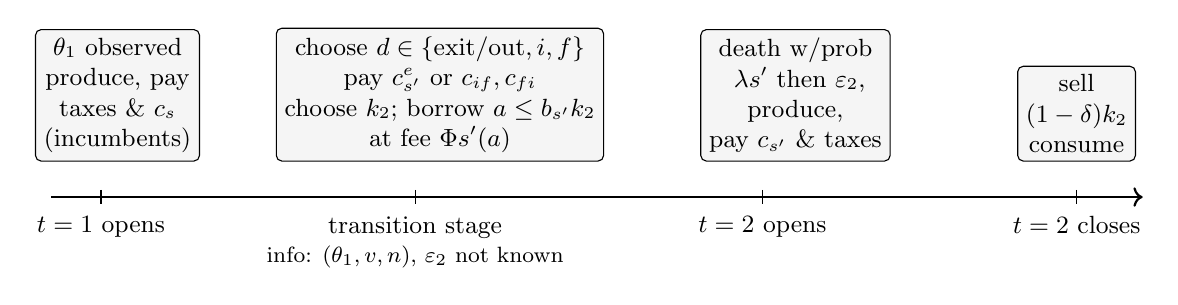
\begin{tikzpicture}[xscale=1.05,
  every node/.style={font=\small},
  decision/.style={draw, rounded corners=2pt, align=center,
                   inner sep=3pt, fill=gray!8}]
  % timeline
  \draw[->, thick] (0,0) -- (13.2,0);
  \foreach \x/\lab in {0.6/{$t=1$ opens}, 4.4/{transition stage},
                       8.6/{$t=2$ opens}, 12.4/{$t=2$ closes}}
    \draw (\x,0.09) -- (\x,-0.09) node[below=1pt] {\lab};
  % events above the line
  \node[decision, anchor=south] at (0.8,0.45)
    {$\theta_1$ observed\\ produce, pay \\
    taxes \& $c_s $ \\
    (incumbents)};
  \node[decision, anchor=south] at (4.7,0.45)
    {choose $d\in\{\text{exit/out},i,f\}$\\
     pay $c^e_{s'}$ or $c_{i f},c_{f i}$\\
     choose $k_2$; borrow $a\le b_{s'}k_2$ \\
     at fee $\Phi{s'}(a)$};
  \node[decision, anchor=south] at (9.0,0.45)
    {death w/prob \\
    \ $\lambda{s'}$ then $\varepsilon_2$, \\
    produce, \\
    pay $c_{s'}$ \& taxes};
  \node[decision, anchor=south] at (12.4,0.45)
    {sell \\ $(1-\delta)k_2$\\ consume};
  % info sets below
  \node[align=center, below=14pt] at (4.4,0)
    {\footnotesize info: $(\theta_1,v,n)$, $\varepsilon_2$
     not known};
\end{tikzpicture}
\end{figure}

\subsection{Static problem: labor demand and the profit function}
\label{sec:toy-static}
 
Let $\tau_y^{s}$ and $\tau_{\ell}^{s}$ denote the taxes effectively paid in sector $s$: $\tau_y^{f}=\tau_y$, $\tau_{\ell}^{f}=\tau_{\ell}$, $\tau_y^{i}=\tau_{\ell}^{i}=0$. Conditional on operating with state $(\theta,k)$, the firm solves $\max_{\ell\geq0}\,(1-\tau_y^{s})\theta k^{\alpha}\ell^{\nu} - (1+\tau_{\ell}^{s})w\,\ell$; substituting the optimal $\ell$ back into the objective yields the operating-profit function

\begin{equation*}
  \pi_{s}(\theta,k)
  \;=\;(1-\nu)\,(1-\tau_y^{s})\,\theta k^{\alpha}
  \left[\frac{\nu\,(1-\tau_y^{s})\,\theta k^{\alpha}}
             {(1+\tau_{\ell}^{s})\,w}\right]^{\frac{\nu}{1-\nu}},
\end{equation*}

which the next lemma rewrites in the separable form used throughout.
 
\begin{lemma}[Labor demand and profits]
\label{lem:static}
Optimal labor and the operating-profit function are
\begin{equation}
  \ell^{*}_{s}(\theta,k)
  = \left[\frac{\nu(1-\tau_y^{s})\,\theta k^{\alpha}}
                {(1+\tau_{\ell}^{s})w}\right]^{\frac{1}{1-\nu}},
  \qquad
  \pi_{s}(\theta,k) \;=\; \Omega_{s}\,x\,k^{\gamma},
  \label{eq:toy-profit}
\end{equation}
where
\begin{equation}
  x \equiv \theta^{\frac{1}{1-\nu}},\qquad
  \gamma \equiv \frac{\alpha}{1-\nu}\in(0,1),\qquad
  \Omega_{s} \equiv (1-\nu)\,(1-\tau_y^{s})^{\frac{1}{1-\nu}}
  \left[\frac{\nu}{(1+\tau_{\ell}^{s})w}\right]^{\frac{\nu}{1-\nu}} .
  \label{eq:toy-omega}
\end{equation}
 Labor demand is strictly increasing in $\theta$ and $k$ ($\partial\ell^{*}/\partial\theta>0$, $\partial\ell^{*}/\partial k>0$) and strictly decreasing in the wage and in own-sector taxes ($\partial\ell^{*}/\partial w<0$, $\partial\ell^{*}_{f}/\partial\tau_y<0$, $\partial\ell^{*}_{f}/\partial\tau_{\ell}<0$). The profit function is strictly increasing and strictly concave in $k$ ($\gamma<1$), and the tax wedge
 
\begin{equation}
  T \;\equiv\; \frac{\Omega_{f}}{\Omega_{i}}
  \;=\; (1-\tau_y)^{\frac{1}{1-\nu}} (1+\tau_{\ell})^{-\frac{\nu}{1-\nu}}
  \;<\;1
  \label{eq:toy-T}
\end{equation}
summarizes the fiscal cost of formality per unit of the profitability
index $\prodx$.
\end{lemma}
 
All proofs are collected in appendix Section~\ref{app:toy-proofs}. The index $x=\theta^{1/(1-\nu)}$ is the natural unit of firm heterogeneity: profits are linear in $x$, so all expectations below reduce to means of a log-normal random variable. Conditional on the transition-stage information set, define the expected profitability index as

\begin{equation}
  \hat x \;\equiv\; \mathbb{E} \!\left[x_{2}\mid \mathcal{I}_{1}\right]
  = \exp\!\left\{\frac{\rho\ln\theta_{1}+(1-\rho)\ln v}{1-\nu}
    + \frac{\sigma_{\varepsilon}^{2}}{2(1-\nu)^{2}}\right\}
  \quad\text{(incumbents)},
  \label{eq:toy-xhat}
\end{equation}


and $\hat x_{e}(v)=\exp\{\ln v/(1-\nu) +\sigma_{\varepsilon}^{2}/(2(1-\nu)^{2})\}$ for entrants (whose period-2 productivity is $\ln\theta_{2}=\ln v+\varepsilon_{2}$). $\hat x$ is strictly increasing in $\theta_{1}$ and in $v$; it is the single sufficient statistic for expected productivity in every decision below.

\subsection{Investment and financing: formal statements}

\begin{lemma}[Capital and borrowing policy]
\label{lem:kpolicy}
The solution to \eqref{eq:toy-Gdef} is
\begin{equation}
  k^{*}_{s}(\hat x,n)=
  \begin{cases}
    \bar{k}_{s}(\hat x), & n \geq \bar{k}_{s}(\hat x)
      \hfill \text{(R1: unconstrained)}\\[3pt]
    n, & \tilde{k}_{s}(\hat x) \le n < \bar{k}_{s}(\hat x)
      \hfill \text{(R2: self-financed at the kink)}\\[3pt]
    \tilde{k}_{s}(\hat x), &
      (1-b_{s})\tilde{k}_{s}(\hat x) \le n <
      \tilde{k}_{s}(\hat x)
      \hfill \qquad \qquad \text{(R3: interior borrowing)}\\[3pt]
    \dfrac{n}{1-b_{s}}, &
      0\le n < (1-b_{s})\tilde{k}_{s}(\hat x)
      \hfill \text{(R4: collateral-constrained)}
  \end{cases}
  \label{eq:toy-kpolicy}
\end{equation}

with borrowing $a^{*}_{s}=\max\{0,k^{*}_{s}-n\}$, strictly positive exactly in R3-R4. This policy is continuous, weakly increasing in $\hat x$ and in $n$, and satisfies the following derivatives

\begin{align}
  \frac{\partial k^{*}_{s}}{\partial \phi_{s}} &=
    -\frac{\tilde{k}_{s}}{(1-\gamma)R_{s}} < 0 \ \text{in R3},
    = 0 \ \text{ow};
  &
  \frac{\partial k^{*}_{s}}{\partial b_{s}} &=
    \frac{n}{(1-b_{s})^{2}} > 0 \ \text{in R4},
    =0 \ \text{ow};
  \notag \\
  \frac{\partial k^{*}_{s}}{\partial n} &= 1 \ \text{in R2},
  \frac{1}{1-b_{s}}>1 \ \text{in R4},
  =0 \ \text{ow};
  &
  \frac{\partial k^{*}_{s}}{\partial \hat x} &> 0
   \ \text{in R1, R3},  =0 \ \text{ow}.
  \label{eq:toy-ksigns}
\end{align}
\end{lemma}
 
Three observations connect Lemma~\ref{lem:kpolicy} to the data. First, investment-cash-flow sensitivity ($\partial k^{*}/\partial n>0$) is positive only for constrained firms (R2, R4), and is largest exactly where the collateral constraint binds (R4). This is the firm-level footprint of the credit channel that the Shift-Share design picks up at the market level. Second, the marginal cost of external funds $\phi_{s}$ acts on the intensive margin of constrained borrowers (R3), while collateral capacity $b_{s}$ acts on the most severely constrained firms (R4), typically young, low-$n$ entrants. Therefore, the two instruments of a credit expansion reach different parts of the firm distribution. Third, borrowing incidence $\mathbb{P}(a^{*}>0)$ rises with expected productivity and falls with internal funds. Finally, notice that this four-region finance-restriction policy is a generalization of the hierarchy of finance with three endogenous regimes of \cite{bond1994dynamic}.
 
\begin{lemma}[Value of operating]
\label{lem:value}
Define $\Psi_{s}(\hat x;R)\equiv(1-\gamma)\,\gamma^{\frac{\gamma}{1-\gamma}} \big(M_{s}\hat x\big)^{\frac{1}{1-\gamma}}R^{-\frac{\gamma}{1-\gamma}}$, which is strictly increasing and strictly convex in $\hat x$ and strictly decreasing in $R$. Then
\begin{equation}
  G_{s}(\hat x,n)=
  \begin{cases}
    \Psi_{s}(\hat x;R^0), & \text{R1}\\[2pt]
    M_{s}\hat x\,n^{\gamma}-R^0 n, & \text{R2}\\[2pt]
    \phi_{s}\,n+\Psi_{s}(\hat x;R_{s}), & \text{R3}\\[2pt]
    \phi_{s}\,n
      + M_{s}\hat x\Big(\tfrac{n}{1-b_{s}}\Big)^{\gamma}
      - R_{s}\,\tfrac{n}{1-b_{s}}, & \text{R4},
  \end{cases}
  \label{eq:toy-G}
\end{equation}
where $G_{s}$ is continuous, strictly increasing and strictly convex in $\hat x$, and
concave and non-decreasing in $n$. Therefore, the marginal value of internal
funds, $q_{s}\equiv 1+\partial G_{s}/\partial n$, satisfies
\begin{equation}
  q_{s}=
  \begin{cases}
    1, & \text{R1}\\[2pt]
    1+\gamma M_{s}\hat x n^{\gamma-1}-R^0\in(1,1+\phi_{s}], & \text{R2}\\[2pt]
    1+\phi_{s}, & \text{R3}\\[2pt]
    1+\phi_{s}
  +\frac{\gamma M_{s}\hat x\,k^{*\,\gamma-1}_{s}-R_{s}}{1-b_{s}}
  \;>\;1+\phi_{s}, & \text{R4},
  \end{cases}
  \label{eq:toy-q}
\end{equation}
 
The step function $q_{s}$ is the shadow price of a peso inside the firm. It exceeds one for constrained firms and jumps above $1+\phi_{s}$ when collateral binds; it is the model object behind the role of entrant wealth $(\muko,\sdko)$ in the quantitative model.
\end{lemma}

\begin{remark}[Borrowing participation and the fixed cost of borrowing]
\label{rem:toy-participation}
In the general model the financing fee has an additional fixed component, $\Phi{s}(a)=\phi_{0s}\mathbf{1}_{a>0}+\phi_{s}\,a$. However, all results in this section extend directly because conditional on borrowing, the fixed cost is sunk. Thus, all policies and envelope derivatives are unchanged, and thresholds are unchanged up to the bookkeeping $m \rightarrow m + \phi_{0s}$ and $C_o \rightarrow C_o + \phi_{0f} - \phi_{0i}$ on branches whose continuation choice is to borrow. Define the borrowing participation premium as the surplus gain from capital expansion using external funds over staying at the kink in capital without external funding,
\begin{equation*}
  \pi^{B}_{s}(\hat x,n)\;\equiv\;
  G_{s}^{\mathrm{R3/R4}}(\hat x,n)
  -\big[M_{s}\hat x\,n^{\gamma}-R^0 n\big],
\end{equation*}
which equals zero at the R2/R3 boundary and is strictly increasing in $\hat x$ beyond it (its $\hat x$-derivative is $M_{s}(k^{*\,\gamma}_{s}-n^{\gamma})>0$ whenever $k^{*}_{s}>n$). With $\phi_{0s}>0$ the firm borrows iff $\pi^{B}_{s}\geq\phi_{0s}$, so the R2/R3 boundary shifts to the unique root of $\pi^{B}_{s}=\phi_{0s}$, which is a borrowing-participation cutoff in $\hat x$ given $n$. The population mass beyond the cutoff, i.e. the borrowing incidence, is strictly decreasing in $\phi_{0s}$ given $(\phi_{s},b_{s})$. The intensive-margin objects ($a^{*}$, the thresholds, their derivatives) in the toy model are unchanged in the quantitative model, conditional on participation.
\end{remark}

The next lemma is the analytical workhorse of the paper. By the envelope theorem, the value of choosing a sector responds to i) its financial conditions in proportion to equilibrium borrowing and ii) to collateral capacity in proportion to the shadow value of pledgeability.
 
\begin{lemma}[Value of financial conditions]
\label{lem:envelope}
Since $G_{s}$, and hence $U_{s}$, are differentiable with respect to $(\phi_{s},b_{s})$, except at region boundaries, we can derive the following derivatives
\begin{equation}
  \frac{\partial U_{s}}{\partial \phi_{s}}
  = -\,a^{*}_{s}(\hat x,n)\;\leq\;0,
  \qquad
  \frac{\partial U_{s}}{\partial b_{s}}
  = \mu_{s}\,k^{*}_{s} \;=\;
  \mathbf{1}_{\mathrm{R4}}\,
  \Big[\gamma M_{s}\hat x\,k^{*\,\gamma-1}_{s}-r_{s}\Big]
  \frac{n}{(1- b_{s})^{2}}\;\geq\;0,
  \label{eq:toy-envelope}
\end{equation}
where $\mu_{s}\geq0$ is the multiplier on \eqref{eq:toy-collateral}. Notice that both inequalities are strict exactly when the firm borrows (respectively, when the collateral constraint binds). Finally, observe that the cross-derivatives are zero: $\partial U_{s}/\partial\phi_{s'}=\partial U_{s}/\partial b_{s'}=0$ for $s'\neq s$.
\end{lemma}

\subsection{Formality threshold}

Define the origin state of a firm as $o\in\{\text{entrant},i\text{-incumbent}, f\text{-incumbent}\}$ and its internal funds available before paying the origin-specific fee of each destination as $n_{o}$. Thus, the destination $s$ leaves internal funds $n_{o,s}=n_{o}-\kappa_{os}$ inside the firm, where $\kappa_{os}\in\{c^e_{s},c_{i f},c_{f i},0\}$ per \eqref{eq:toy-n}. Then, the firm's formality decision compares

\begin{equation}
  \Delta_{o}(\hat x,n_{o}) \;\equiv\;
  U_{f}(\hat x,n_{o}-\kappa_{of})
  -U_{i}(\hat x,n_{o}-\kappa_{oi}) .
\end{equation}

Notice that the empirically relevant region for this comparison is R3 for both destinations. This is growing firms whose desired capital exceeds its internal funds. The statement below is for that region R3, and Section~\ref{app:toy-proofs} verifies that the threshold structure extends piecewise to R2/R4 (and characterizes the cash-rich case in Remark~\ref{rem:toy-rich}). On origin $\times$ destination region R3 $\times$ R3, the following expression holds
 
\begin{equation}
  \Delta_{o}(\hat x,n_{o})
  = A\,\hat x^{\frac{1}{1-\gamma}}
  \;-\; B\,n_{o} \;-\; C_{o},
  \label{eq:toy-Delta-affine}
\end{equation}

where 

\begin{align}
  A &\equiv (1-\gamma)\,\gamma^{\frac{\gamma}{1-\gamma}}
      \left[ M_{f}^{\frac{1}{1-\gamma}}R_{f}^{-\frac{\gamma}{1-\gamma}}
           - M_{i}^{\frac{1}{1-\gamma}}R_{i}^{-\frac{\gamma}{1-\gamma}}
      \right],
  \qquad
  B \equiv \phi_{i}-\phi_{f} \;>\;0,
  \label{eq:toy-AB}\\[2pt]
  C_{o} &\equiv (1+\phi_{f})\,\kappa_{of}
        - (1+\phi_{i})\,\kappa_{oi}
        + \beta\big[(1-\lambda_{f})c_{f}
                   -(1-\lambda_{i})c_{i}\big] .
  \label{eq:toy-C}
\end{align}
 
\begin{assumption}[Finance-driven formality]
\label{ass:A1}
Define $T_{\lambda}\equiv T\cdot\dfrac{1-\lambda_{f}}{1-\lambda_{i}}$ as the tax wedge adjusted by the survival advantage of formality. Then

\begin{equation}
  \left(\frac{R_{f}}{R_{i}}\right)^{\gamma}
  \;<\; T_{\lambda} .
  \label{eq:toy-A1}
\end{equation}
\end{assumption}
 
Assumption~\ref{ass:A1} states that, for a firm that has to borrow, the financing advantage of formality ($\left(\frac{R_{f}}{R_{i}}\right)^{\gamma} < 1$) outweighs its fiscal cost net of the survival advantage ($T_{\lambda} \lessgtr 1$). This assumption is equivalent to $A>0$, and it is the exact sense in which formality is, in this model, access to capital. Absent a financing or survival advantage ($R_{f}=R_{i}$, $\lambda{f}=\lambda{i}$), $T<1$ implies $A<0$ and no borrower would ever formalize.
 
\begin{assumption}[Interior thresholds and cost ordering]
\label{ass:A2}
(a) $C_{o}+B\,n_{o}>0$, means that the fixed and transition costs of formality are not dominated by its switching benefits. (b) The switching and entry fees satisfy $c_{if},c_{fi}>0$, $0\leq c^e_{i}\leq c^e_{f}$, and

\begin{align}
  (1+\phi_{f})\,c^e_{f}-(1+\phi_{i})\,c^e_{i}
  \;&<\;(1+\phi_{f})\,c_{if},
  \tag{A2-i}\label{eq:toy-A2i}\\
  (1+\phi_{f})\,c^e_{f}+(1+\phi_{i})\,c_{fi}
  \;&>\;(1+\phi_{i})\,c^e_{i}.
  \tag{A2-ii}\label{eq:toy-A2ii}
\end{align}
\end{assumption}

Conditions (A2-i) and (A2-ii) are exactly equivalent to a cost ordering that places the entrant formality threshold strictly between the two incumbent thresholds, with the formal incumbent facing the lowest cost of formality and the informal incumbent the highest: (A2-i) says that entering formal is cheaper than entering informal and immediately formalizing, and (A2-ii) says that entering informally is cheaper than entering formally and immediately switching down, which holds automatically whenever the switch-down fee is at least the informal entry fee, and in particular whenever informal entry is nearly free, the empirically relevant case (Appendix~\ref{app:toy-details} states the cost-ordering lemma).

\begin{proposition}[Formality threshold]
\label{prop:threshold}
Under Assumptions~\ref{ass:A1}--\ref{ass:A2}, for each origin $o$ and internal funds $n_{o}$, $\Delta_{o}(\cdot,n_{o})$ is strictly increasing and strictly convex in $\hat x$ and crosses zero exactly once, at
\begin{equation}
  \hat x^F_{o}(n_{o})
  \;=\;\left[\frac{B\,n_{o}+C_{o}}{A}\right]^{1-\gamma} .
  \label{eq:toy-threshold}
\end{equation}
Thus, the firm chooses the formal sector if and only if $\prodxhat\geq\thF{o}(n_{o})$. The threshold is strictly increasing in internal funds, so
\begin{equation}
  \frac{\partial \hat x^F_{o}}{\partial n_{o}}
  = (1-\gamma)\,\frac{B}{A}
    \left[\frac{Bn_{o}+C_{o}}{A}\right]^{-\gamma} \;>\;0,
  \label{eq:toy-dthdn}
\end{equation}
this is, conditional on expected productivity, firms with more internal funds are less likely to formalize, because self-finance substitutes for the financial advantage of formality.
\end{proposition}
 
Proposition~\ref{prop:threshold} formalizes the sorting logic of the model. The firms that select into formality are those whose growth needs are large relative to their internal resources, i.e. high $\hat x$, low $n$. These are precisely the firms for which a bank credit supply shock is decisive, which is why the Shift-Share elasticities of Section~\ref{results} are informative about $(\spread{s},\collat{s})$.

For unconstrained, cash-rich firms the finance advantage is irrelevant, and with taxes as the only non-financial difference a sufficiently wealthy firm prefers informality; a strong enough survival advantage of formality ($T_\lambda \ge 1$) or the size-dependent audit cost of the general model removes this artifact, and the sizable mass of formal-to-informal transitions in the data suggests that for many firms the net non-financial advantage of formality is indeed weak (Appendix~\ref{app:toy-details}).
 
\subsection{The full transition map and its comparative statics}
\label{sec:toy-map}

Each exit and entry margin reduces to one comparison, continuation in the informal sector (the relevant alternative at low $\hat{x}$, by the ordering below) against consuming the outside value, and each is characterized by a condition of the form $G_s(\hat{x}, \tilde{n}) = m$, where $\tilde{n}$ are the funds carried into the continuation and $m$ collects the operating and transition costs. Solving branch by branch of the financing regions yields a single master threshold whose four instances are exit from either sector and entry into either sector; Appendix~\ref{app:toy-details} states it and Appendix~\ref{app:toy-taxonomy} develops the complete taxonomy. Two of its properties matter below: a firm without internal funds exits or fails to enter at any productivity (financial exit), and a constrained firm whose quasi-rents on internal funds cover the relevant costs never exits. The thresholds are ordered as follows.
 
\begin{proposition}[Ordered thresholds]
\label{prop:ordering}
Under Assumptions~\ref{ass:A1}--\ref{ass:A2} and
$c_{i}>0$, for each level of internal funds the policy of every origin state is a partition of the $\hat x$ line, such that $ \hat x_i^X < \hat x_i^E < \hat x_f^X < \hat x_f^I < \hat x_f^E < \hat x_i^F $,

\begin{center}
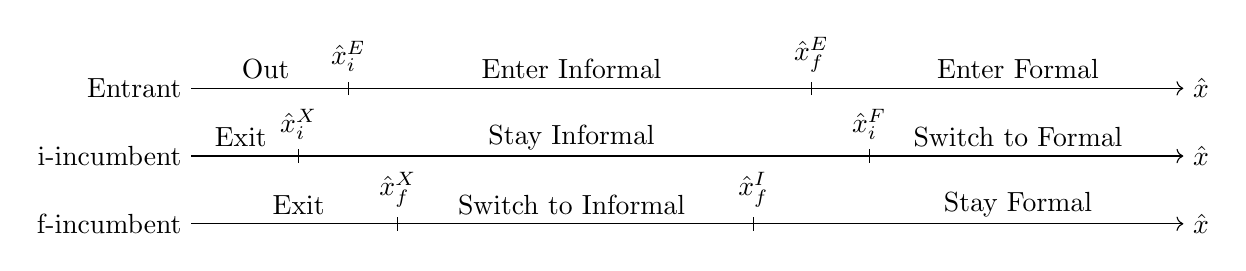
\begin{tikzpicture}[xscale=1.05, yscale=0.86, every node/.style={font=\normalsize}]
  % entrant line
  \draw[->] (0,2) -- (12,2) node[right] {$\hat x$};
  \node[left] at (0,2) {Entrant};
  \foreach \x/\lab in {1.9/{$\hat x_i^E$}, 7.5/{$\hat x_f^E$}}
    \draw (\x,1.9) -- (\x,2.1) node[above] {\lab};
  \node at (0.9,2.28) {Out};
  \node at (4.6,2.28) {Enter Informal};
  \node at (10,2.28) {Enter Formal};
  % informal incumbent
  \draw[->] (0,1) -- (12,1) node[right] {$\hat x$};
  \node[left] at (0,1) {i-incumbent};
  \foreach \x/\lab in {1.3/{$\hat x_i^X$}, 8.2/{$\hat x_i^F$}}
    \draw (\x,0.9) -- (\x,1.1) node[above] {\lab};
  \node at (0.6,1.28) {Exit};
  \node at (4.6,1.28) {Stay Informal};
  \node at (10,1.28) {Switch to Formal};
  % formal incumbent
  \draw[->] (0,0) -- (12,0) node[right] {$\hat x$};
  \node[left] at (0,0) {f-incumbent};
  \foreach \x/\lab in {2.5/{$\hat x_f^X$}, 6.8/{$\hat x_f^I$}}
    \draw (\x,-0.1) -- (\x,0.1) node[above] {\lab};
  \node at (1.3,0.28) {Exit};
  \node at (4.6,0.28) {Switch to Informal};
  \node at (10,0.28) {Stay Formal};
\end{tikzpicture}
\end{center}
\end{proposition}

\subsection{Cost ordering and the cash-rich region}

Notice that conditions \eqref{eq:toy-A2i}-\eqref{eq:toy-A2ii} are exactly equivalent (by Lemma~\ref{lem:costorder} below) to the cost ordering $C_{f\text{-inc}}<C_{\text{entrant}}<C_{i\text{-inc}}$ that places the entrant formality threshold between the two incumbent thresholds. \eqref{eq:toy-A2i} says that enter as formal is cheaper than enter as informal and immediately formalize; \eqref{eq:toy-A2ii} says that entering informally is cheaper than entering formally and immediately switching to formal. \eqref{eq:toy-A2ii} holds automatically whenever $\swc{\fml\infml}\geq\ec{\infml}$, and in particular whenever informal entry is (nearly) free, the empirically relevant case.
 
\begin{lemma}[Cost ordering]
\label{lem:costorder}
Evaluate \eqref{eq:toy-C} at each origin's fee pair $(\kappa_{of},\kappa_{oi})$\footnote{$(c_{if},0)$ for informal incumbents, $(0,c_{fi})$ for formal incumbents, $(c^e_{f},c^e_{i})$ for entrants} and define $K\equiv\beta[(1-\lambda{f})c_{f}-(1-\lambda{i})c_{i}]$. Then the costs are
\begin{equation}
  C_{i\text{-inc}}=(1+\phi_{f})c_{if}+K,\quad
  C_{f\text{-inc}}=-(1+\phi_{i})c_{fi}+K,\quad
  C_{e}=(1+\phi_{f})c^e_{f}-(1+\phi_{i})c^e_{i}+K,
  \label{eq:toy-Cvalues}
\end{equation}
and $C_{e}<C_{i\text{-inc}}\iff$\eqref{eq:toy-A2i}, while $C_{f\text{-inc}}<C_{e}\iff$\eqref{eq:toy-A2ii}. Under $c_{if},c_{fi}>0$ alone, $C_{f\text{-inc}}<C_{i\text{-inc}}$ always holds; \eqref{eq:toy-A2i}--\eqref{eq:toy-A2ii} are what places the entrant threshold strictly inside these two costs.
\end{lemma}

\begin{remark}[Cash-rich firms and the role of the audit margin]
\label{rem:toy-rich}
For unconstrained firms (R1 $\times$ R1) the finance advantage is irrelevant and $\text{sgn} \{\Delta_{o}\} = \text{sgn}\{\Psi_{f}(\hat x;R^0) -\Psi_{i}(\hat x;R^0)-\text{costs}\}$, which under $T_{\lambda}<1$ is negative for large $\hat x$. This means that with taxes as the only non-financial difference, a sufficiently wealthy firm prefers informality. Two observations discipline this artifact. First, with $\lambda{i}>\lambda{f}$ large enough, $T_{\lambda}\geq1$ and formality remains absorbing even for the cash-rich. The sizable mass of formal-to-informal transitions in the data, on average $286$ per market and window against $310$ formalizations (Section~\ref{results}), suggests that for many firms the net non-financial advantage of formality is weak, that is, $T_{\lambda}$ close to or below one; the quantitative model lets the data settle this through $(\tau_{y},\tau_{\ell},\lambda_{s},\eta_{i})$.
\end{remark}

\subsection{The master threshold and its four instances}

Combining the exit option with Proposition~\ref{prop:threshold} yields the complete policy map of each origin state, mirroring the decision rules $s_{n},s_{i},s_{f}$ of the quantitative model. 

Every exit and entry margin reduces to one comparison, continuation in the informal sector (the relevant alternative at low $\hat x$, by the ordering of Proposition~\ref{prop:ordering}) against consuming the outside value. Define

\begin{equation}
  A_{s}\equiv(1-\gamma)\Big(\frac{\gamma}{R_{s}}\Big)^{\frac{\gamma}{1-\gamma}}
  M_{s}^{\frac{1}{1-\gamma}},\quad
  A^{0}_{s}\equiv(1-\gamma)\Big(\frac{\gamma}{R^0}\Big)^{\frac{\gamma}{1-\gamma}}
  M_{s}^{\frac{1}{1-\gamma}},\quad
  \mathcal{K}_{s}\equiv\beta(1-\lambda_{s})c_{s},
  \label{eq:toy-Anot}
\end{equation}

so that $\Psi_{s}(\prodxhat;\Rext{s})=A_{s}\prodxhat^{1/(1-\curv)}$, and define the identities $A=A_{f}-A_{i}$ for the formality-margin slope in \eqref{eq:toy-AB} and $A^{0}=A^{0}_{f}-A^{0}_{i}$ for the cash-rich slope of Remark~\ref{rem:toy-rich}. Each margin is characterized by a condition of the form $G_{s}(\prodxhat,\tilde\netw)=m$, where $\tilde\netw$ are the funds carried into the continuation and $m$ collects the operating and transition costs. Solving branch by branch of \eqref{eq:toy-G} defines the following master threshold

\begin{equation}
  \mathcal{X}_{s}(\tilde n;m)\;=\;
  \begin{cases}
    \big(m/A^{0}_{s}\big)^{1-\gamma},
      & \text{R1}\\[4pt]
    \dfrac{m+R^0\tilde n}{M_{s}\,\tilde n^{\gamma}},
      & \text{R2}\\[8pt]
    \left[\dfrac{m-\phi_{s}\tilde n}{A_{s}}\right]^{1-\gamma},
      & \text{R3, if } m>\phi_{s}\tilde n\\[8pt]
    (1-b_{s})^{\gamma}\,
    \dfrac{m+\tilde n\,\dfrac{R^0+\phi_{s}b_{s}}
    {1-b_{s}}}{M_{s}\,\tilde n^{\gamma}},
      & \text{R4},
  \end{cases}
  \label{eq:toy-master}
\end{equation}

where $\mathcal{X}_{s}$ is continuous across the R1/R2, R2/R3 and R3/R4 boundaries, weakly decreasing in $\tilde n$, independent of financial conditions on R1, and satisfies $\mathcal{X}_{s}\to\infty$ as $\tilde n\to0^{+}$ on R4. Notice that firms without internal funds exit or fail to enter at any productivity (financial exit). Moreover, on R2, $G_{s}$ is linear in $\hat x$, hence the no power form. If $m\leq\phi_{s}\tilde n$ on R3 (or the analogous condition on R4), the constrained firm never exits because the quasi-rents $\phi_ {s}\tilde n$ earned by internal funds keep it alive at any productivity.
 
Hence, the four thresholds are instances of \eqref{eq:toy-master}:
\begin{align}
  \text{Exit as informal:}\quad
  &\hat x^X_{i}(n)=\mathcal{X}_{i}\big(n;\;\mathcal{K}_{i}\big),
  &&n=n^{\text{exit}},
  \label{eq:toy-thXi}\\[2pt]
  \text{Exit as formal:}\quad
  &\hat x^X_{f}(n)=\mathcal{X}_{i}\big(n-c_{fi};\;
    \mathcal{K}_{i}+c_{fi}\big),
  &&n=n^{\text{exit}},
  \label{eq:toy-thXf}\\[2pt]
  \text{Entry as informal:}\quad
  &\hat x^E_{i}(k_{0})=\mathcal{X}_{i}\big(k_{0}-c^e_{i};\;
    \mathcal{K}_{i}+c^e_{i}\big),
  \label{eq:toy-thEi}\\[2pt]
  \text{Entry as formal:}\quad
  &\hat x^E_{f}(k_{0})=\hat x^F_{e}(k_{0})
    =\left[\frac{B\,k_{0}+C_{e}}{A}\right]^{1-\gamma}
  &&\text{(Prop.~\ref{prop:threshold})} .
  \label{eq:toy-thEf}
\end{align}

% Three things to notice from this master threshold. i) In \eqref{eq:toy-thXf} the formal incumbent's relevant alternative to exiting is switching down (below $\hat x^F_{f}$ staying formal is dominated by Proposition~\ref{prop:ordering}), so the comparison is $U_{i}(\hat x,n-c_{fi})\gtrless n$. On region R3 the numerator of \eqref{eq:toy-master} becomes $\mathcal{K}_{i}+(1+\phi_{i})c_{fi} -\phi_{i} n$, which is the switch fee priced at the informal shadow price of funds, exactly as in Lemma~\ref{lem:costorder}. ii) Likewise on R3, the entry margin \eqref{eq:toy-thEi} has numerator $\mathcal{K}_{i}+(1+\phi_{i})c^e_{i} -\phi_{i}k_{0}$, and on R4 it inherits $\hat x^E_{i}\to\infty$ as $k_{0}\downarrow c^e_{i}$: wealth-constrained non-entry in the spirit of \cite{evans1989estimated}. \emph{(iii)} Under Assumption~\ref{ass:A2} the ordering $\thE{\infml}(k_{0})<\thF{e}(k_{0})$ makes the formality margin the binding condition for formal entry in \eqref{eq:toy-thEf}; the direct enter-formal-versus-out threshold, relevant only outside that ordering, is $\Xth{\fml}(k_{0}-\ec{\fml};\Kop{\fml}+\ec{\fml})$. In primitive units, entrant thresholds convert through $\bar{v}(k_{0})=\big[\hat{x}^{\bullet}(k_{0})\big]^{1-\nu} \exp\{-\sigma_{\varepsilon}^{2}/(2(1-\nu))\}$ and incumbent thresholds through \eqref{eq:toy-thbar}. 

A complete taxonomy of these thresholds is developed in appendix Section~\ref{app:toy-taxonomy}.

\subsection{Comparative statics}
\label{app:comparative_stats}
 
\begin{proposition}[Comparative statics of all thresholds]
\label{prop:statics}
On the borrowing regions, with $D_{o}\equiv Bn_{o}+C_{o}>0$ and
$a^{*}_{s}$ evaluated at the relevant margin, the thresholds respond to financial conditions as follows:
% (``$0$'' means zero except through inactive regions):
\begin{center}
\small
\renewcommand{\arraystretch}{1.7}
\begin{tabular}{lcccc}
\hline
 & $\phi_{f}\uparrow$ & $\phi_{i}\uparrow$
 & $b_{f}\uparrow$ & $b_{i}\uparrow$ \\
\hline
Formality margins
$\hat x^F_{e},\hat x^F_{i},\hat x^F_{f}$ &
$\dfrac{(1-\gamma)\,a^{*}_{\fml}}{D_{o}}>0$ &
$-\dfrac{(1-\gamma)\,a^{*}_{i}}{D_{o}}<0$ &
$\leq 0$ &
$\geq 0$ \\
Informal entry/exit $\hat x^E_{i},\hat x^X_{i}$ &
$0$ &
$\dfrac{a^{*}_{i}}{\Psi'_{i}}>0$ &
$0$ &
$\leq 0$ \\
Formal exit $\hat x^X_{f}$ &
$0$ &
$\dfrac{a^{*}_{i}}{\Psi'_{i}}>0$ &
$ 0$ &
$\leq 0$ \\
\hline
\multicolumn{5}{@{}p{0.97\linewidth}@{}}{\footnotesize\emph{Note}: entries assume the threshold ordering of Proposition~\ref{prop:ordering}, so the formal incumbent's relevant alternative at its exit margin is the switch-down option; off that ordering the formal-exit row picks up $\geq0$ ($\phi_{f}$) and $\leq0$ ($b_{f}$) terms through the value of staying formal. The first row reports $\partial\ln(\text{threshold})/ \partial(\text{parameter})$; the second and third rows report level derivatives, with $a^{*}_{i}$ evaluated at the margin's funds ($n$ for informal exit/entry, $n-c_{fi}$ for formal exit).}\\
\end{tabular}
\end{center}

\end{proposition}

\subsection{Transition semi-elasticities}

The thresholds translate into transition probabilities, the objects the Shift-Share design estimates, by integrating over the period-1 population. Consider informal incumbents with permanent component $v$ and internal funds $n$ (the same algebra applies to each origin state). Since $\ln\theta_{1}=\ln v+\varepsilon_{1}$ and $\hat x$ is monotone in $\theta_{1}$, the probability of an informal-to-formal switch is

\begin{equation}
  \mathbb{P}(i\to f \mid v,n)
  = 1-\Phi\!\left(z_{if}\right),
  \qquad
  z_{if} \equiv\frac{\ln\bar{\theta}_{if}(v,n)-\ln v}{\sigma_{\varepsilon}},
  \label{eq:toy-Pif}
\end{equation}
where the productivity threshold inverts \eqref{eq:toy-xhat}:
\begin{equation}
  \ln\bar{\theta}_{if}(v,n)
  = \frac{1}{\rho}\Big[(1-\nu)\ln \hat x^F_{i}(n)
  - (1-\rho)\ln v\Big]
  - \frac{\sigma_{\varepsilon}^{2}}{2\rho(1-\nu)} .
  \label{eq:toy-thbar}
\end{equation}

Expression \eqref{eq:toy-thbar} is common to all regions. Its derivation uses only the log-linear map \eqref{eq:toy-xhat} and the existence of a cutoff in $\hat x$-units, so it converts any threshold, whichever branch of \eqref{eq:toy-master} delivers it, closed-form or implicit, into a cutoff for $\theta_{1}$. The financing region enters only through the value of the threshold and through its derivatives in the chain rule below. Analogous expressions hold for $\mathbb{P}(\text{exit}\mid \infml)=\Phi(z_{\infml X})$, $\mathbb{P}(\fml\to\infml)=\Phi(z_{\fml\infml})-\Phi(z_{\fml X})$, entry probabilities (with $\hat x_{e}(v)$ and thresholds in $v$), and all the other transitions.

\subsection{From thresholds to transition rates}
\label{sec:toy-transitions}

Integrating over the period-1 population translates the thresholds into transition probabilities, the objects the Shift-Share design estimates: each transition probability is a normal probability of the standardized gap between log productivity and the operative threshold, so the response of any transition rate to financial conditions is the density of firms at the margin times the threshold shift of the comparative statics above, scaled by borrowing at the relevant margin. Appendix~\ref{app:toy-details} derives the semi-elasticity of every transition rate in closed form; self-financed firms contribute exactly zero, and aggregate responses are incidence-weighted integrals that concentrate among small, young, low-net-worth firms near their thresholds. The payoff for the empirical strategy is the incidence algebra of the switching margins.

% The analytical workhorse of the paper is the envelope pair $\partial U_s/\partial \phi_s = -\,a_s^*(\hat{x}, n) \le 0$ and $\partial U_s/\partial b_s = \mu_s k_s^* \ge 0$, with $\mu_s$ the multiplier on the collateral constraint and zero cross-derivatives, $\partial U_s/\partial \phi_{s'} = \partial U_s/\partial b_{s'} = 0$ for $s' \ne s$: the value of choosing a sector responds to its own financial conditions in proportion to equilibrium borrowing, to its own collateral capacity in proportion to the shadow value of pledgeability, and to the other sector's terms not at all, with both own-sector responses strict exactly for borrowers. In the general model the financing fee carries an additional fixed component $\phi_{0s}\,\mathbf{1}\{a>0\}$; conditional on borrowing the fixed cost is sunk, so all policies and envelope derivatives are unchanged, and the borrowing-participation cutoff it creates is the moment that identifies the fixed cost at estimation (Appendix~\ref{app:toy-details}).
 
\begin{corollary}[Incidence and the switching margins]
\label{cor:bothmargins}
Consider a credit supply expansion that improves both sectors'
borrowing terms: spreads fall by the absolute amounts
$\varepsilon_{s}\equiv\chi_{s}\spread{s}\geq0$, i.e.\
$\diff\spread{s}=-\varepsilon_{s}$, and/or collateral capacities
rise, $\diff\collat{s}\geq0$. The conditions below are stated for
the spread components; a collateral improvement adds
$\mu_{s}k^{*}_{s}\diff\collat{s}$ to its own sector's side of each
inequality. Then:
\begin{enumerate}
    \item[(i)] \emph{Entry and exit.} Under Proposition~\ref{prop:ordering}, the binding entry margin and both exit margins, $\thE{\infml}$, $\thX{\infml}$, $\thX{\fml}$, are informal-continuation comparisons, so they respond only to informal-side terms: all three fall when $\varepsilon_{\infml}>0$ or $\diff\collat{\infml}>0$, and are unchanged under a purely formal-side expansion. Hence total entry rises and exit falls at both incumbent margins whenever the expansion reaches the informal side; the formal/informal \emph{composition} of entry is governed by $\thF{e}$, which obeys the same condition as the switching margins of (ii).
    \item[(ii)] \emph{Switching up.} $\Prob(\infml\to\fml)$ rises if and only if
    \begin{equation}
        \varepsilon_{\fml}\,a^{*}_{\fml}
        \;>\;
        \varepsilon_{\infml}\,a^{*}_{\infml}
        \qquad\text{at the } \infml\to\fml \text{ margin.}
        \label{eq:toy-ifcond}
    \end{equation}
    Because the switch fee travels with the formal option, $a^{*}_{\fml}-a^{*}_{\infml}
    =\tilde{k}_{\fml}-\tilde{k}_{\infml}+\swc{\infml\fml}>0$ under Assumption~\ref{ass:A1}; hence equal absolute improvements ($\varepsilon_{\fml}=\varepsilon_{\infml}$) always raise informal-to-formal switching. Under equal \emph{proportional} improvements ($\chi_{\fml}=\chi_{\infml}$), \eqref{eq:toy-ifcond} reads $\spread{\fml}a^{*}_{\fml}>\spread{\infml}a^{*}_{\infml}$: the borrowing-scale gap must outweigh the spread gap. The same condition, with the $a^{*}$'s evaluated at the entrant's funds ($a^{*}_{s}=\tilde{k}_{s}-(k_{0}-\ec{s})$), governs the entrant margin $\thF{e}$: there $a^{*}_{\fml}-a^{*}_{\infml} =\tilde{k}_{\fml}-\tilde{k}_{\infml}+\ec{\fml}-\ec{\infml}>0$, so equal absolute improvements also raise the formal share of entrants.
    \item[(iii)] \emph{Switching down.} $\Prob(\fml\to\infml)$ rises if and only if
    \begin{equation}
        \varepsilon_{\infml}\,a^{*}_{\infml}
        \;>\;
        \varepsilon_{\fml}\,a^{*}_{\fml}
        \qquad\text{at the } \fml\to\infml \text{ margin,}
        \label{eq:toy-ficond}
    \end{equation}
    where now the fee travels with the informal option,
    $a^{*}_{\infml}-a^{*}_{\fml}
    =\tilde{k}_{\infml}-\tilde{k}_{\fml}+\swc{\fml\infml}$. Both switching margins can therefore rise together only if the expansion has a sufficiently informal-side component
    ($\varepsilon_{\infml}$, or $\collat{\infml}\uparrow$).
\end{enumerate}

\end{corollary}

This incidence algebra is the toy model's central payoff for the empirical strategy, and the estimates of Section~6 discipline it. Formalization rises and de-formalization falls; by (ii) and (iii) both movements require the same inequality, that the formal-side improvement dominates at each switching margin, $\varepsilon_f a_f^* > \varepsilon_i a_i^*$, while the size of the de-formalization decline is informative about the informal side, because a larger informal-side improvement attenuates it. The entry and exit block points the same way: informal entry is flat and exit rises, so the informal-side threshold effects of (i) are absent from the data, and the exit increase instead reflects the turnover of marginal cohorts, the subject of the next subsection. The estimated switching pattern is thereby converted into a statement about which sector's borrowing terms the shock reached, and this is the restriction taken to the structural estimation: the first-stage credit response and the collateral response pin the formal-side incidence, the two switching responses discipline the informal-side loading, which the data keep small, and the interest rate is kept as a measurement equation rather than an estimation target.
 
\subsection{Composition: marginal entrants, turnover, and average productivity}
\label{sec:toy-composition}

The last set of results concerns the composition of the response. This is where the model meets the value-added estimates of Section~\ref{results}: informal value added falls, formal value added does not move, and the average across firms is at most marginally positive. Allow period-2 firms a shutdown option: after observing $\theta_{2}$, an active firm operates iff variable profit covers the fixed cost, $\Om{s}\prodx_{2}k_{2}^{\curv}\geq \fc{s}$; otherwise it stays idle for the period (it still resells its capital). Shutdown is the two-period analogue of endogenous exit for a young cohort. For an entering cohort into sector $\infml$ (the same algebra applies to a formal entering cohort, the margin the estimated shock moves most), entry occurs iff $v\geq \bar{v}(k_{0})$, where $\bar v$ solves $\prodxhat_{e}(\bar v)=\thE{\infml}(k_{0})$, and:

\begin{equation}
  \mathbb{P}(\text{shutdown of an entrant with} (v,k_{2})):
  \pi^{X}(v)=\Phi\!\left(
  \frac{(1-\nu)\ln\!\big(\fc{\infml}/(\Om{\infml}k_{2}^{\curv})\big)
        -\ln v}{\sigma_{\varepsilon}}\right),
  \label{eq:toy-shutdown}
\end{equation}
which is strictly decreasing in $v$ (directly, and indirectly through
$k_{2}$).
 
\begin{proposition}[Composition of a credit expansion]
\label{prop:composition}
Let financial conditions improve for the informal sector
($\spread{\infml}\downarrow$ or $\collat{\infml}\uparrow$), so that
$\bar v$ falls for every constrained $k_{0}$. Then, for the entering
cohort:
\begin{enumerate}
\item[(i)] \emph{Entry rises}: the mass of entrants
  $\int\Prob(v\geq\bar v(k_{0}))\,\diff F(k_{0})$ increases.
\item[(ii)] \emph{Average entrant productivity falls}: for
  $\ln v\sim N(0,\sdv^{2})$,
  $\E[v\mid v\geq\bar v]$ is strictly increasing in $\bar v$; hence a
  lower threshold mechanically lowers the mean (and every quantile) of
  entrant productivity, and with it average value added per entrant.
\item[(iii)] \emph{Cohort turnover rises}: the cohort shutdown rate
  $\E[\pi^{X}(v)\mid v\geq\bar v]$ is strictly decreasing in
  $\bar v$; the marginal entrants admitted by the expansion fail at
  higher rates than infra-marginal ones, so measured exit rises with a
  lag even as incumbent exit thresholds fall.
\end{enumerate}
\end{proposition}

Part~(iii) of the proposition isolates the composition channel: for the collateral- constrained entrants where the margin lives, capital is pinned by wealth and collateral, so a pure spread reduction leaves their capital unchanged and the composition effect is the entire response, while a collateral relaxation deepens their capital and partially offsets it. The proposition thus reproduces, inside the two-period model, the composition signature of Section~6: the expansion admits marginal, lower-$v$ entrants and raises their subsequent turnover, the model counterpart of the estimated exit response, while on the informal side the formality threshold falls, the most productive informal firms leave the pool, and informal average value added declines. The two forces lower average productivity within the informal sector, the response that is robust in the data, and leave the economy-wide average roughly flat, exactly as estimated: the model reads the value-added results as reallocation plus selection, not as productivity gains within infra-marginal firms.
 
\begin{proposition}[Transition semi-elasticities]
\label{prop:semielast}
Define $p=\mathbb{P}(i\to f \mid v,n)$ from \eqref{eq:toy-Pif}. Then, when both destinations borrow at an interior optimum (R3) at the margin,

\begin{equation}
  \frac{\partial p}{\partial \phi_{f}}
  = -\,\phi(z_{if})\,
     \frac{(1-\nu)(1-\gamma)}{\rho\,\sigma_{\varepsilon}}\,
     \frac{a^{*}_{f}}{D_{i}} \;<\;0,
  \qquad
  \frac{\partial p}{\partial \phi_{i}}
  = \phi(z_{if})\,
     \frac{(1-\nu)(1-\gamma)}{\rho\,\sigma_{\varepsilon}}\,
     \frac{a^{*}_{i}}{D_{i}} \;>\;0,
  \label{eq:toy-dpdphi}
\end{equation}

while, when the relevant destination is collateral-constrained (R4) at the margin, the collateral responses are

\begin{equation}
  \frac{\partial p}{\partial b_{f}}
  = \phi(z_{if})\,
     \frac{1-\nu}{\rho\,\sigma_{\varepsilon}}\,
     \frac{\mu_{f}k^{*}_{f}}{N_{i}} \;\geq\;0,
  \qquad
  \frac{\partial p}{\partial b_{i}}
  = -\,\phi(z_{if})\,
     \frac{1-\nu}{\rho\,\sigma_{\varepsilon}}\,
     \frac{\mu_{i}k^{*}_{i}}{N_{i}} \;\leq\;0,
  \label{eq:toy-dpdb}
\end{equation}

where $N_{i}$ is the numerator of the operative branch of $\hat x^F_{i}$ at the crossing\footnote{Which is equal to $D_{i}\hat x^{*}$ on R4$\times$R4. See appendix Section~\ref{app:toy-taxonomy} for more details.} and $\mu_{s}k^{*}_{s}$ is the shadow value of collateral of Lemma~\ref{lem:envelope}. The same structure, with the appropriate threshold and sign from Proposition~\ref{prop:statics}, applies to every other transition probability. The factor $(1-\curv)$ is specific to the power branch (R3) and drops on the linear branches; all responses are scaled by $\phi(z)/\sigma_{\varepsilon}$, which is the density of firms at the margin, so aggregate responses are largest where the firm distribution is thick near thresholds.
\end{proposition}
 
Two aggregation implications worth highlighting. First, because \eqref{eq:toy-thbar} is region-free, the chain rule composes with whichever region's log-derivative is operative at the margin for the given $(v,n)$. Thus, the $\phi$-formulas displayed are the R3 instances, the collateral formulas the R4 instances, and R1/R2 self-financed firms contribute exactly zero. Second, aggregate transition responses are therefore incidence-weighted integrals. This is $\phi(z)$ times the region-specific term, integrated over the joint distribution of $(v,n)$, that concentrates predicted responses among small, young, low-net-worth firms. Which is the sample counterpart of the heterogeneity documented in Section~\ref{results}.

\subsection{The model-implied estimand in closed form}

Finally, the toy model makes precise what the Leave-One-Out Shift-Share
coefficient identifies through the lens of the model. Appendix \ref{app:estimand} shows as an example the detailed case of the effect on the mass of informal firms. The quantitative model computes this object numerically; the generic case presented here is schematic and serves to draw general conclusions. Let the
bank-supply shock in market $m$ shift financial conditions by
$\diff\Xi_{m}
=(-\chi_{\infml}\spread{\infml},-\chi_{\fml}\spread{\fml},
\kappa_{\infml}\collat{\infml},\kappa_{\fml}\collat{\fml})'\,
\zeta_{m}$, where $\zeta_{m}$ is the (exogenous) shock intensity.
Aggregate borrowing is
$C=\int a^{*}\,\diff\mu$ over active firms, and each firm-count outcome
$Y$ (stocks, entry, exit, transitions by sector) aggregates the
threshold rules. To first order, the model counterpart of the IV
estimand is the ratio of two equilibrium responses to the \emph{same}
financial-conditions shift:

\begin{equation}
  \beta_{Y}^{\text{model}}
  \;=\;
  \frac{\diff\ln Y/\diff\zeta}{\diff\ln C/\diff\zeta}
  \;=\;
  \frac{\displaystyle\sum_{j\in\text{margins of }Y}
        \frac{\phi(z_{j})}{Y}\,
        \frac{(1-\nu)(1-\curv)}{\rho\sigma_{\varepsilon}}
        \frac{\spread{}\,a^{*}\chi}{D_{j}} }
       {\displaystyle \frac{1}{C} \Big[\underbrace{\int_{borrowers}
        \frac{\chi_{s'} \phi_{s'} \tilde{k}_{s'}(\hat{x})}{(1-\gamma)R_{s'}}\diff\mu}_{\text{intensive: loan deepening}}
        -\underbrace{\sum_{j} \int w_M s_M \Delta a^{*}_{j} \diff \mu }_{\text{extensive: Created/swapped loans}}\Big]} ,
  \label{eq:toy-estimand}
\end{equation}

where $w_M$ and $s_M$ are as defined in Appendix \ref{app:estimand}. Three lessons that carry to the quantitative model. First, the numerator is a density-weighted sum of threshold shifts: the IV coefficient is large where many firms sit near their thresholds, young, small, constrained firms, which rationalizes why the gross-flow elasticities (entry, exit, switching) exceed the net stock response, since flows add up threshold crossings while the stock nets them out, and why the responses concentrate on the formal side, the sector whose borrowing terms the shock improves. Second, the denominator mixes intensive responses (continuing borrowers deepen loans by $\chi_{s}\spread{s}\tilde k_{s}/[(1-\curv)\Rext{s}]$ each) with extensive ones (loans created and swapped at the margins), and both are built from parameters estimated off cross-sectional moments, spread levels, participation costs, collateral caps. Matching the observed first stage disciplines that financing block directly: the quantity response pins $\chi_{f}\phi_{f}$ and the collateral response pins $\kappa_{f}$, while the loan-rate response is kept as a measurement check rather than a target, because the observed book rate mixes repricing with near-complete turnover of the loan stock. Third, because $\zeta$ enters numerator and denominator symmetrically, $\beta^{\text{model}}_{Y}$ is invariant to the scale of the shock for small $\zeta$: the model counterpart can be computed from any small perturbation, and only the incidence $(\chi_{\infml},\chi_{\fml},\kappa_{\fml})$, not the size, of the credit supply shock needs to be estimated $\kappa_{\infml}=0$ in the baseline: bank credit supply shocks do not shift informal collateral technology).

\section{Proofs}
\label{app:toy-proofs}
 
\begin{proof}[Proof of Lemma~\ref{lem:static}]
The objective
$(1-\taxy^{s})\theta k^{\alpha}\ell^{\nu}-(1+\taxl^{s})w\ell$ is
strictly concave in $\ell$ ($\nu<1$); the first-order condition
$\nu(1-\taxy^{s})\theta k^{\alpha}\ell^{\nu-1}=(1+\taxl^{s})w$ gives
$\ell^{*}_{s}$ in \eqref{eq:toy-profit}. Substituting, using
$(1+\taxl^{s})w\,\ell^{*}=\nu(1-\taxy^{s})\theta k^{\alpha}
\ell^{*\nu}$, yields
$\prof{s}=(1-\nu)(1-\taxy^{s})\theta k^{\alpha}\ell^{*\nu}$ and, after
substituting $\ell^{*\nu}$, expression \eqref{eq:toy-omega}. Monotonicity
claims follow by inspection of the closed forms:
$\partial\ln\ell^{*}/\partial\ln\theta=1/(1-\nu)>0$,
$\partial\ln\ell^{*}/\partial\ln k=\alpha/(1-\nu)>0$,
$\partial\ln\ell^{*}/\partial\ln w=-1/(1-\nu)<0$, and both tax terms
enter with negative sign. Strict concavity of $\prof{s}$ in $k$ follows
from $\curv=\alpha/(1-\nu)<1$, itself implied by $\alpha+\nu<1$.
$T<1$ is immediate from $\taxy,\taxl>0$.
\end{proof}
 
\begin{proof}[Proof of Lemma~\ref{lem:kpolicy}]
The objective in \eqref{eq:toy-Gdef} is continuous and, on each branch
of $a=\max\{0,k-\netw\}$, strictly concave in $k$ (the return term has
curvature $\curv<1$; the cost terms are linear). Marginal return to
capital is $g'(k)=\curv M_{s}\hat x k^{\curv-1}+\beta(1-\delta)$,
strictly decreasing, with range $(\beta(1-\delta),\infty)$. Marginal
cost is $1$ for $k<\netw$ and $1+\spread{s}$ for $k>\netw$. If
$g'(\netw)\leq 1$, i.e.\ $\netw\geq\bar k_{s}$, the self-financed
optimum $\bar k_{s}$ (where $g'=1$) is attainable without borrowing:
region R1. If $1<g'(\netw)\leq 1+\spread{s}$, i.e.\
$\tilde k_{s}\leq\netw<\bar k_{s}$, the kink at $k=\netw$ is optimal:
region R2. If $g'(\netw)>1+\spread{s}$, i.e.\ $\netw<\tilde k_{s}$, the
firm borrows to the interior optimum $\tilde k_{s}$ (where
$g'=1+\spread{s}$) provided the collateral constraint
$k-\netw\leq\collat{s}k \iff k\leq\netw/(1-\collat{s})$ permits, i.e.\
$\tilde k_{s}\leq \netw/(1-\collat{s})$: region R3. Otherwise the
constraint binds and $k=\netw/(1-\collat{s})$: region R4. The
boundaries in \eqref{eq:toy-kpolicy} restate these conditions. The
derivative signs follow from
$\tilde k_{s}=(\curv M_{s}\hat x/\Rext{s})^{1/(1-\curv)}$ and
$\bar k_{s}=(\curv M_{s}\hat x/\Rint)^{1/(1-\curv)}$, so that
$\partial\tilde k_{s}/\partial\spread{s}
=-\tilde k_{s}/[(1-\curv)\Rext{s}]$,
$\partial\tilde k_{s}/\partial\hat x
=\tilde k_{s}/[(1-\curv)\hat x]$ and
$\partial\bar k_{s}/\partial\hat x
=\bar k_{s}/[(1-\curv)\hat x]$;
from $k=\netw/(1-\collat{s})$ in R4, whose $\collat{s}$-derivative is
$\netw/(1-\collat{s})^{2}$; and by inspection elsewhere.
Continuity at boundaries is direct substitution.
\end{proof}
 
\begin{proof}[Proof of Lemma~\ref{lem:value}]
Substitute the policy \eqref{eq:toy-kpolicy} into
\eqref{eq:toy-Gdef}. R1: $G=M_{s}\hat x\bar k^{\curv}-\Rint\bar k$;
using $\curv M_{s}\hat x\bar k^{\curv-1}=\Rint$,
$G=\Rint\bar k(1-\curv)/\curv=\Psi_{s}(\hat x;\Rint)$ after
substituting $\bar k$. R2: $k=\netw$, $a=0$:
$G=M_{s}\hat x\netw^{\curv}-\Rint\netw$. R3:
$G=-\tilde k-\spread{s}(\tilde k-\netw)
+M_{s}\hat x\tilde k^{\curv}+\beta(1-\delta)\tilde k
=\spread{s}\netw+M_{s}\hat x\tilde k^{\curv}-\Rext{s}\tilde k$, and
the same substitution with $\Rext{s}$ gives
$\spread{s}\netw+\Psi_{s}(\hat x;\Rext{s})$. R4: substitute
$k=\netw/(1-\collat{s})$ directly. Monotonicity and convexity of
$\Psi_{s}$ in $\hat x$ follow from the exponent
$1/(1-\curv)>1$; $G$ inherits them. The formulas for $q_{s}$ are the
$\netw$-derivatives of \eqref{eq:toy-G}; the R2 bounds follow because
$g'(\netw)\in(1,1+\spread{s}]$ there, and the R4 inequality because the
bracketed marginal-return gap is strictly positive when the collateral
constraint binds. Concavity of $G$ in $\netw$ holds piecewise and at
kinks because $q_{s}$ is (weakly) decreasing in $\netw$ region by
region as $\netw$ rises through R4$\to$R3$\to$R2$\to$R1.
\end{proof}
 
\begin{proof}[Proof of Lemma~\ref{lem:envelope}]
On R1--R2, $a^{*}=0$ and $(\spread{s},\collat{s})$ do not enter the
realized objective: derivatives are zero, consistent with
\eqref{eq:toy-envelope}. On R3--R4 apply the envelope theorem to
\eqref{eq:toy-Gdef}: the derivative of the value with respect to
$\spread{s}$ at the optimum is the partial derivative of the objective,
$-a^{*}_{s}$; for $\collat{s}$, the constraint $a\leq\collat{s}k$ has
multiplier $\mu_{s}\geq0$ and the envelope derivative is
$\mu_{s}k^{*}_{s}$, zero when slack (R3) and equal to the stated
expression in R4, where the Kuhn--Tucker condition gives
$\mu_{s}=\big[\curv M_{s}\hat x k^{*\curv-1}-\Rext{s}\big]
/(1-\collat{s})\cdot$(normalization); differentiating \eqref{eq:toy-G}
in R4 with respect to $\collat{s}$ directly yields
$\big[\curv M_{s}\hat x k^{*\curv-1}_{s}-\Rext{s}\big]\,
\netw/(1-\collat{s})^{2}>0$. Cross-sector derivatives are zero because
$s'$-parameters do not enter sector-$s$ payoffs.
\end{proof}
 
\begin{proof}[Proof of Proposition~\ref{prop:threshold}]
On R3$\times$R3, \eqref{eq:toy-Delta-affine} follows by subtracting the
R3 branch of \eqref{eq:toy-G} for each destination and collecting the
$\hat x^{1/(1-\curv)}$, $\netw_{o}$, and constant terms, using
\eqref{eq:toy-n}. $A>0$ iff
$M_{\fml}^{1/(1-\curv)}\Rext{\fml}^{-\curv/(1-\curv)}
>M_{\infml}^{1/(1-\curv)}\Rext{\infml}^{-\curv/(1-\curv)}$, i.e.\ iff
$M_{\fml}/M_{\infml}>(\Rext{\fml}/\Rext{\infml})^{\curv}$; since
$M_{\fml}/M_{\infml}=T_{\lambda}$ by definition, this is
Assumption~\ref{ass:A1}. Strict monotonicity and convexity in
$\hat x$ follow from $A>0$ and the exponent $1/(1-\curv)>1$; since
$\Delta_{o}\to -(B\netw_{o}+C_{o})<0$ as $\hat x\to0$ (by
Assumption~\ref{ass:A2}) and $\Delta_{o}\to\infty$ as $\hat x\to\infty$, a unique zero
exists and solves \eqref{eq:toy-threshold}. Differentiating
\eqref{eq:toy-threshold} in $\netw_{o}$ gives \eqref{eq:toy-dthdn}.
For completeness, off R3$\times$R3 the difference
$\Delta_{o}$ remains continuous and strictly increasing in $\hat x$
wherever the formal destination is in a (weakly) more constrained
region than the informal one, which holds at the crossing point under
Assumption~\ref{ass:A1} because $\tilde k_{\fml}>\tilde k_{\infml}$
(shown in the proof of Corollary~\ref{cor:bothmargins}); hence the
crossing is unique globally on the borrowing range.
\end{proof}
\begin{proof}[Proof of Lemma~\ref{lem:costorder}]
Substituting each origin's fee pair into
\eqref{eq:toy-C} gives \eqref{eq:toy-Cvalues} directly; the common
constant $K$ cancels from every pairwise difference. Upper comparison:
\begin{equation*}
  C_{\infml\text{-inc}}-C_{e}
  =(1+\spread{\fml})\swc{\infml\fml}
   -\big[(1+\spread{\fml})\ec{\fml}-(1+\spread{\infml})\ec{\infml}\big]
  \;>\;0
  \iff \text{\eqref{eq:toy-A2i}} .
\end{equation*}
Lower comparison:
\begin{equation*}
  C_{e}-C_{\fml\text{-inc}}
  =(1+\spread{\fml})\ec{\fml}-(1+\spread{\infml})\ec{\infml}
   +(1+\spread{\infml})\swc{\fml\infml}
  \;>\;0
  \iff \text{\eqref{eq:toy-A2ii}} .
\end{equation*}
Note that $\ec{\infml}\leq\ec{\fml}$ alone does \emph{not} imply
\eqref{eq:toy-A2ii}, because $\spread{\infml}>\spread{\fml}$ can make
$(1+\spread{\infml})\ec{\infml}$ exceed
$(1+\spread{\fml})\ec{\fml}$; if
$\swc{\fml\infml}\geq\ec{\infml}$, however,
$(1+\spread{\infml})(\swc{\fml\infml}-\ec{\infml})\geq0$ and
$(1+\spread{\fml})\ec{\fml}>0$ deliver \eqref{eq:toy-A2ii}. Finally,
$C_{\infml\text{-inc}}-C_{\fml\text{-inc}}
=(1+\spread{\fml})\swc{\infml\fml}
+(1+\spread{\infml})\swc{\fml\infml}>0$ under positive switching fees
alone.
\end{proof}
 
\begin{proof}[Proof of Proposition~\ref{prop:ordering}]
The three-interval structure for each origin follows from: (i) values
of continuation are continuous and strictly increasing in $\hat x$
while exit/out values are constant in $\hat x$, giving unique
exit/entry cutoffs; (ii) Proposition~\ref{prop:threshold} gives the
unique formality cutoff above them whenever
$\thX{}<\thF{}$, which holds under Assumption~\ref{ass:A2} (the
formality margin requires strictly positive net cost $D_{o}>0$ while
the exit margin turns on $\fc{\infml}$); the formal incumbent's middle
interval is switching down rather than staying informal by
definition of its choice set. The ordering
$\thF{\fml}<\thF{e}<\thF{\infml}$ follows from
\eqref{eq:toy-threshold}: thresholds are increasing in $C_{o}$, and
$C_{\fml\text{-inc}}<C_{\text{entrant}}<C_{\infml\text{-inc}}$ by
Assumption~\ref{ass:A2}.
\end{proof}
 
\begin{proof}[Proof of Proposition~\ref{prop:statics}]
Each threshold is defined by an indifference condition
$\Delta(\hat x^{*},\cdot)=0$ between two options. By the implicit
function theorem,
$\partial\hat x^{*}/\partial\xi
=-(\partial\Delta/\partial\xi)/(\partial\Delta/\partial\hat x)$,
and $\partial\Delta/\partial\hat x>0$ at an upward crossing. The
numerators are given by Lemma~\ref{lem:envelope}: for the formality
margins, $\partial\Delta/\partial\spread{\fml}=-a^{*}_{\fml}$,
$\partial\Delta/\partial\spread{\infml}=+a^{*}_{\infml}$,
$\partial\Delta/\partial\collat{\fml}=\mu_{\fml}k^{*}_{\fml}\geq0$,
$\partial\Delta/\partial\collat{\infml}=-\mu_{\infml}k^{*}_{\infml}
\leq0$. Using
$\partial\Delta/\partial\hat x
=A\hat x^{\curv/(1-\curv)}/(1-\curv)
=D_{o}/[(1-\curv)\hat x^{*}]$ at the threshold (substituting
$A\hat x^{*1/(1-\curv)}=D_{o}$) delivers the log-derivatives in the
first row. For the informal entry/exit margins the indifference is
$G_{\infml}=\text{const}$, so
$\partial\Delta/\partial\spread{\infml}=-a^{*}_{\infml}$ and
$\partial\Delta/\partial\hat x=\Psi'_{\infml}>0$, giving the stated
positive derivative (thresholds rise as informal finance becomes
dearer); formal-side parameters do not enter, hence the zeros. For
formal exit, the relevant comparison at low $\hat x$ under the
ordering of Proposition~\ref{prop:ordering} is exit versus switching
down, whose value is
$\Uv{\infml}(\hat x,\netw-\swc{\fml\infml})$; its derivatives in
informal financial parameters are those of $\Uv{\infml}$
(Lemma~\ref{lem:envelope}), delivering the third row's informal-side
entries, and formal-side parameters do not enter the comparison at
all, hence its zeros. Off that ordering --- if staying formal were the
binding alternative at the exit margin --- the cutoff would be
$\Xth{\fml}(\netw;\Kop{\fml})$ and easier formal terms would weakly
lower it ($\geq0$ in $\spread{\fml}$, $\leq0$ in $\collat{\fml}$),
which is the caveat recorded in the table note.
\end{proof}
 
\begin{proof}[Proof of Proposition~\ref{prop:semielast}]
$p=1-\Phi(z)$ with
$z=(\ln\bar\theta-\ln v)/\sigma_{\varepsilon}$ and, from
\eqref{eq:toy-thbar},
$\partial\ln\bar\theta/\partial\xi
=\frac{1-\nu}{\rho}\,\partial\ln\thF{\infml}/\partial\xi$ for any
financial parameter $\xi$. Chain-differentiate and substitute the
log-derivatives from Proposition~\ref{prop:statics};
$\phi(\cdot)>0$ delivers the signs. For \eqref{eq:toy-dpdb}: on the
linear branches the threshold is the ratio of a linear numerator to a
slope (Section~\ref{app:toy-taxonomy}); the quotient rule with the
root identity $N_{\infml}=D_{4}\hat x^{*}$ gives
$\partial\ln\thF{\infml}/\partial\collat{\fml}
=-\mu_{\fml}k^{*}_{\fml}/N_{\infml}$ and
$\partial\ln\thF{\infml}/\partial\collat{\infml}
=+\mu_{\infml}k^{*}_{\infml}/N_{\infml}$, and the same chain rule
applies; the $(1-\curv)$ factor is absent because the operative branch
is linear in $\hat x$.
\end{proof}
 
\begin{proof}[Proof of Corollary~\ref{cor:bothmargins}]
\emph{(i)} Under Proposition~\ref{prop:ordering} the binding entry
margin and both exit margins compare an \emph{informal} continuation
with the outside value, so by Lemma~\ref{lem:envelope} they respond
only to informal-side terms (second and third rows of
Proposition~\ref{prop:statics}): all three thresholds fall when
$\varepsilon_{\infml}>0$ or $\diff\collat{\infml}>0$, and total entry, the mass of entrants above $\thE{\infml}$, rises.

\emph{(ii)--(iii)} By Lemma~\ref{lem:envelope}, total differentiation
of the formality margin of origin $o$ gives
\begin{equation*}
  \diff\Delta_{o}
  =-a^{*}_{\fml}\,\diff\spread{\fml}
   +a^{*}_{\infml}\,\diff\spread{\infml}
  =\varepsilon_{\fml}a^{*}_{\fml}-\varepsilon_{\infml}a^{*}_{\infml},
\end{equation*}
so $\thF{o}$ falls, formality gains ground, if and only if
$\varepsilon_{\fml}a^{*}_{\fml}>\varepsilon_{\infml}a^{*}_{\infml}$.
Since $p_{\infml\to\fml}$ falls in $\thF{\infml}$ while
$p_{\fml\to\infml}$ rises in $\thF{\fml}$, this is
\eqref{eq:toy-ifcond} at the $\infml\to\fml$ margin and, reversed,
\eqref{eq:toy-ficond} at the $\fml\to\infml$ margin. For the
borrowing gaps: at the $\infml\to\fml$ margin the formal option
carries funds $\netw-\swc{\infml\fml}$ and the informal option
$\netw$, so
\begin{equation*}
  a^{*}_{\fml}-a^{*}_{\infml}
  =\big[\tilde{k}_{\fml}-(\netw-\swc{\infml\fml})\big]
   -\big[\tilde{k}_{\infml}-\netw\big]
  =\tilde{k}_{\fml}-\tilde{k}_{\infml}+\swc{\infml\fml}.
\end{equation*}

For the entrant margin the fee pair $(\ec{\fml},\ec{\infml})$ gives
$a^{*}_{\fml}-a^{*}_{\infml}
=\tilde{k}_{\fml}-\tilde{k}_{\infml}+\ec{\fml}-\ec{\infml}$, so the
same argument applies to $\thF{e}$.

Under Assumption~\ref{ass:A1},
$T_{\lambda}>(\Rext{\fml}/\Rext{\infml})^{\curv}$ implies
$T_{\lambda}\,\Rext{\infml}/\Rext{\fml}
>(\Rext{\infml}/\Rext{\fml})^{1-\curv}>1$, hence
$\tilde{k}_{\fml}/\tilde{k}_{\infml}
=\big(T_{\lambda}\Rext{\infml}/\Rext{\fml}\big)^{1/(1-\curv)}>1$:
the gap is strictly positive, and
$\varepsilon_{\fml}=\varepsilon_{\infml}$ delivers
\eqref{eq:toy-ifcond}. At the $\fml\to\infml$ margin the fee switches
sides, $a^{*}_{\infml}-a^{*}_{\fml}
=\tilde{k}_{\infml}-\tilde{k}_{\fml}+\swc{\fml\infml}$, giving the
statement in (iii).
\end{proof}

\begin{proof}[Proof of Proposition~\ref{prop:composition}]
(i) The entry threshold $\bar v$ falls by
Proposition~\ref{prop:statics} (second row), so the entry probability
$1-F_{v}(\bar v)$ rises for every $k_{0}$ with a constrained margin.
(ii) For a log-normal $v$ the truncated mean
$m(\bar v)\equiv\E[v\mid v\geq\bar v]$ satisfies
$m'(\bar v)=h(\bar v)\,[m(\bar v)-\bar v]>0$, where
$h=f_{v}/(1-F_{v})$ is the hazard and $m(\bar v)>\bar v$; hence a lower
threshold strictly lowers the truncated mean, and first-order
stochastic dominance of the truncated distributions delivers the same
for every quantile and for average value added (an increasing transform
of $v$). (iii) Write the cohort shutdown rate as
$S(\bar v)=\E[\pi^{X}(v)\mid v\geq\bar v]$ with $\pi^{X}$ strictly
decreasing (by \eqref{eq:toy-shutdown} and
$\partial k_{2}/\partial v\geq0$). Then
$S'(\bar v)=h(\bar v)\big[S(\bar v)-\pi^{X}(\bar v)\big]<0$ because
$\pi^{X}(\bar v)>\pi^{X}(v)$ for all $v>\bar v$ implies
$\pi^{X}(\bar v)>S(\bar v)$. A lower $\bar v$ therefore raises the
cohort shutdown rate.
\end{proof}

\section{Explicit instance of the estimand: informality mass}
\label{app:estimand}
Fix the outcome $Y=N'_{\infml}$, the mass choosing the informal
sector at the transition stage (survival $1-\death{\infml}$
multiplies the measured stock but cancels from $\diff\ln Y$). Six
thresholds delimit it: informal incumbents contribute the band
$[\thX{\infml},\thF{\infml})$, formal incumbents the switch-down
band $[\thX{\fml},\thF{\fml})$, and entrants the interval
$[\bar v^{E},\bar v^{F})$ in type units. Assume the empirically
relevant financing regions (R3 at every one-sided margin,
R3$\times$R3 at the formality margins); on R4-financed margins the
formulas below pick up the collateral terms
($\mu k^{*}$, $\kappa_{s}\collat{s}$) per the taxonomy appendix.
For each margin $M$, contracting Proposition~\ref{prop:statics} with
the shock
$(\diff\spread{s},\diff\collat{s})
=(-\chi_{s}\spread{s},\kappa_{s}\collat{s})\,\diff\zeta$ gives the
log-shift per unit of intensity,
\begin{align*}
  s_{M} &= -(1-\curv)\,\chi_{\infml}\spread{\infml}\,
    \frac{a^{*}_{\infml,M}}{N_{M}},
  && M\in\{X_{\infml},\,X_{\fml},\,E\}
     \ \text{(one-sided, i-continuation)},\\[2pt]
  s_{F,o} &= -\frac{1-\curv}{D_{o}}
    \Big[\chi_{\fml}\spread{\fml}\,a^{*}_{o\fml}
    -\chi_{\infml}\spread{\infml}\,a^{*}_{o\infml}\Big],
  && o\in\{\infml,\fml,e\}
     \ \text{(formality margins)},
\end{align*}
with $(\tilde\netw_{M},m_{M})$ each margin's funds--cost pair,
$N_{M}=m_{M}-\spread{\infml}\tilde\netw_{M}$ the operative R3
numerator, and all $a^{*}$'s evaluated at the crossing. The density
weights at the margins are
$w_{M}=\frac{1-\nu}{\rho\sigma_{\varepsilon}}\,\phi(z_{M})$ for
incumbent margins and
$w_{M}=(1-\nu)\,f_{v}(\bar v_{M})\,\bar v_{M}$ for entrant margins
(entry decisions are deterministic in $v$, so the relevant density is
that of the type distribution). Writing $\iota_{M}=+1$ if an upward
crossing of $M$ moves a firm \emph{into} $Y$ and $-1$ if out of it
($\iota=+1$ at $X_{\infml},X_{\fml},E$; $\iota=-1$ at
$F_{\infml},F_{\fml},F_{e}$), the reduced form is
\begin{equation}
  \frac{\diff\ln N'_{\infml}}{\diff\zeta}
  \;=\;
  -\frac{1}{N'_{\infml}}
  \sum_{M}\iota_{M}\int w_{M}\,s_{M}\;\diff\mu_{o(M)},
  \label{eq:toy-estimand-num}
\end{equation}
each integral taken over the origin population carrying margin $M$.
The first stage decomposes into the loan-size response of continuing
borrowers and the loans created or swapped at the same six margins:
\begin{equation}
  \frac{\diff\ln C}{\diff\zeta}
  \;=\;
  \frac{1}{C}\Bigg[
  \sum_{s'\in\{\infml,\fml\}}
  \int_{\text{borrowers to }s'}
  \frac{\chi_{s'}\spread{s'}\,\tilde k_{s'}(\hat x)}
       {(1-\curv)\,\Rext{s'}}\;\diff\mu
  \;-\;
  \sum_{M}\int w_{M}\,s_{M}\,\Delta a^{*}_{M}\;\diff\mu_{o(M)}
  \Bigg],
  \label{eq:toy-estimand-den}
\end{equation}
where $\Delta a^{*}_{M}$ is the borrowing gained on an upward
crossing: the new loan $a^{*}_{\infml,M}$ at $X_{\infml},X_{\fml},E$
(exit and non-entry carry no loan), and the destination swap
$\Delta a^{*}_{F,o}
=\tilde k_{\fml}-\tilde k_{\infml}+\kappa_{o\fml}-\kappa_{o\infml}$
at the formality margins --- precisely the borrowing gaps of
Corollary~\ref{cor:bothmargins}. The model coefficient is the ratio
$\beta^{\text{model}}_{N_{\infml}}
=\big(\diff\ln N'_{\infml}/\diff\zeta\big)\big/
\big(\diff\ln C/\diff\zeta\big)$; every term in
\eqref{eq:toy-estimand-num}--\eqref{eq:toy-estimand-den} is linear in
the incidence $(\chi_{\infml},\chi_{\fml},\kappa_{\fml})$, so the
scale of $\zeta$ cancels.

\section{Complete threshold taxonomy}
\label{app:toy-taxonomy}
 
This appendix reports the fully substituted closed form of every
exit and entry threshold on every financing region. Throughout,
$\Kop{s}\equiv\beta(1-\death{s})\fc{s}$ (so that
$K=\Kop{\fml}-\Kop{\infml}$),
$A_{s}=(1-\curv)(\curv/\Rext{s})^{\frac{\curv}{1-\curv}}
M_{s}^{\frac{1}{1-\curv}}$ and
$A^{0}_{s}=(1-\curv)(\curv/\Rint)^{\frac{\curv}{1-\curv}}
M_{s}^{\frac{1}{1-\curv}}$, with $A=A_{\fml}-A_{\infml}$ and
$A^{0}=A^{0}_{\fml}-A^{0}_{\infml}$. Each one-sided margin (exit or
entry against the outside option, informal continuation being the
relevant alternative by Proposition~\ref{prop:ordering}) is the
solution of $G_{\infml}(\prodxhat,\tilde\netw)=m$ with the
margin-specific pair $(\tilde\netw,m)$:
\begin{center}
\renewcommand{\arraystretch}{1.35}
\begin{tabular}{lccl}
\hline
margin & $\tilde\netw$ & $m$ & comparison \\
\hline
exit as informal & $\netw$ & $\Kop{\infml}$
  & $\Uv{\infml}(\prodxhat,\netw)\gtrless\netw$ \\
exit as formal & $\netw-\swc{\fml\infml}$ & $\Kop{\infml}+\swc{\fml\infml}$
  & $\Uv{\infml}(\prodxhat,\netw-\swc{\fml\infml})\gtrless\netw$ \\
entry as informal & $k_{0}-\ec{\infml}$ & $\Kop{\infml}+\ec{\infml}$
  & $\Uv{\infml}(\prodxhat,k_{0}-\ec{\infml})\gtrless k_{0}$ \\
\hline
\end{tabular}
\end{center}
with $\netw=\netw^{\text{exit}}$ of \eqref{eq:toy-n}. Substituting the
four branches of \eqref{eq:toy-G}:
 
\textbf{Exit as informal.}
\begin{equation}
  \thX{\infml}(\netw)=
  \begin{cases}
    \big(\Kop{\infml}/A^{0}_{\infml}\big)^{1-\curv},
      & \text{R1}\\[3pt]
    \dfrac{\Kop{\infml}+\Rint\netw}{M_{\infml}\,\netw^{\curv}},
      & \text{R2}\\[8pt]
    \left[\dfrac{\Kop{\infml}-\spread{\infml}\netw}
    {A_{\infml}}\right]^{1-\curv},
      & \text{R3, if } \Kop{\infml}>\spread{\infml}\netw\\[8pt]
    (1-\collat{\infml})^{\curv-1}\,
    \dfrac{\Kop{\infml}(1-\collat{\infml})
    +\netw\big(\Rint+\spread{\infml}\collat{\infml}\big)}
    {M_{\infml}\,\netw^{\curv}},
      & \text{R4}.
  \end{cases}
  \label{eq:app-thXi}
\end{equation}
 
\textbf{Exit as formal (against switching down).}
\begin{equation}
  \thX{\fml}(\netw)=
  \begin{cases}
    \big[(\Kop{\infml}+\swc{\fml\infml})/A^{0}_{\infml}\big]^{1-\curv},
      & \text{R1}\\[3pt]
    \dfrac{\Kop{\infml}+\swc{\fml\infml}
    +\Rint(\netw-\swc{\fml\infml})}
    {M_{\infml}\,(\netw-\swc{\fml\infml})^{\curv}},
      & \text{R2}\\[8pt]
    \left[\dfrac{\Kop{\infml}+(1+\spread{\infml})\swc{\fml\infml}
    -\spread{\infml}\netw}{A_{\infml}}\right]^{1-\curv},
      & \text{R3, if numerator}>0\\[8pt]
    (1-\collat{\infml})^{\curv-1}\,
    \dfrac{(\Kop{\infml}+\swc{\fml\infml})(1-\collat{\infml})
    +(\netw-\swc{\fml\infml})
    \big(\Rint+\spread{\infml}\collat{\infml}\big)}
    {M_{\infml}\,(\netw-\swc{\fml\infml})^{\curv}},
      & \text{R4}.
  \end{cases}
  \label{eq:app-thXf}
\end{equation}
 
\textbf{Entry as informal.}
Replace $(\netw,\swc{\fml\infml})$ by $(k_{0},\ec{\infml})$ in
\eqref{eq:app-thXf}; in particular on R3,
\begin{equation}
  \thE{\infml}(k_{0})
  =\left[\frac{\Kop{\infml}+(1+\spread{\infml})\ec{\infml}
  -\spread{\infml}k_{0}}{A_{\infml}}\right]^{1-\curv},
  \label{eq:app-thEi}
\end{equation}
and in type units
$\bar{v}(k_{0})=\thE{\infml}(k_{0})^{\,1-\nu}
\exp\{-\sigma^{2}_{\varepsilon}/(2(1-\nu))\}$.
 
\textbf{Entry as formal (the entrant formality margin).}
This margin compares two continuation values, each on its own region,
with funds $\tilde\netw_{\fml}=k_{0}-\ec{\fml}$ and
$\tilde\netw_{\infml}=k_{0}-\ec{\infml}$. Because
$G_{s}(\cdot,\tilde\netw)$ is a power function of $\prodxhat$ on
R1/R3 but \emph{linear} in $\prodxhat$ on R2/R4, closed forms obtain
on the diagonal region pairs:
\begin{align}
  \text{R3}\times\text{R3:}\quad
  &\thF{e}(k_{0})=\left[\frac{B\,k_{0}+C_{e}}{A}\right]^{1-\curv},
  \qquad C_{e}=(1+\spread{\fml})\ec{\fml}
  -(1+\spread{\infml})\ec{\infml}+K;
  \label{eq:app-thEf33}\\[2pt]
  \text{R1}\times\text{R1:}\quad
  &\thF{e}=\big(C^{0}_{e}/A^{0}\big)^{1-\curv},
  \qquad C^{0}_{e}=\ec{\fml}-\ec{\infml}+K,
  \label{eq:app-thEf11}\\
  &\text{(direction of the inequality per the trichotomy of
  Remark~\ref{rem:toy-rich})};\notag\\[2pt]
  \text{R2}\times\text{R2:}\quad
  &\thF{e}=\frac{K+\beta(1-\delta)\big(\ec{\fml}-\ec{\infml}\big)}
  {M_{\fml}\tilde\netw_{\fml}^{\curv}
  -M_{\infml}\tilde\netw_{\infml}^{\curv}},
  \qquad\text{formal above iff the denominator $>0$}
  \label{eq:app-thEf22}\\
  &\text{(at kink, only cost is forgone resale value, hence }\beta(1-\delta)\text{, not }\Rint);\notag\\[2pt]
  \text{R4}\times\text{R4:}\quad
  &\thF{e}=\frac{K+\Rext{\fml}h_{\fml}-\Rext{\infml}h_{\infml}
  +(1+\spread{\infml})\tilde\netw_{\infml}
  -(1+\spread{\fml})\tilde\netw_{\fml}}
  {M_{\fml}h_{\fml}^{\curv}-M_{\infml}h_{\infml}^{\curv}},
  \label{eq:app-thEf44}\\
  &\text{with } h_{s}\equiv\tilde\netw_{s}/(1-\collat{s})
  \text{ the capital installed at the binding cap}.\notag
\end{align}
Off-diagonal pairs (one destination borrowing while the other
self-finances, e.g.\ R3$\times$R2) mix
$\prodxhat^{1/(1-\curv)}$ and $\prodxhat$ terms: the indifference
condition remains strictly monotone in $\prodxhat$ at the crossing and
has a unique root, but no closed form; it is solved implicitly. The
same diagonal/off-diagonal taxonomy applies verbatim to the incumbent
formality margins $\thF{\infml},\thF{\fml}$ with the fee pairs of
Lemma~\ref{lem:costorder}.

\textbf{Branch selection.}
Which branch applies is a self-consistency requirement: compute the
candidate threshold from each branch and retain the one whose funds
fall in that branch's bracket \emph{evaluated at the candidate},
\begin{equation*}
  \text{R1: }\tilde\netw\geq\bar{k}_{s}(\prodxhat^{*});\quad
  \text{R2: }\tilde{k}_{s}(\prodxhat^{*})\leq\tilde\netw
  <\bar{k}_{s}(\prodxhat^{*});\quad
  \text{R3: }(1-\collat{s})\tilde{k}_{s}(\prodxhat^{*})
  \leq\tilde\netw<\tilde{k}_{s}(\prodxhat^{*});\quad
  \text{R4: below.}
\end{equation*}

Exactly one branch is self-consistent: $G_{s}$ is continuous and
strictly increasing in $\prodxhat$
($\partial G_{s}/\partial\prodxhat=M_{s}k^{*\curv}>0$ by the envelope
theorem), and at fixed $\tilde\netw$ the firm moves monotonically
through R1$\to$R2$\to$R3$\to$R4 as $\prodxhat$ rises, so
$G_{s}(\cdot,\tilde\netw)$ crosses any constant $m$ exactly once.

\section{Discussion of modeling assumptions}
\label{sec:gen-discussion}

Holding the wage fixed is the exact analogue of the empirical identification, which is within market and year and purged of aggregate shocks, and it is additionally supported by local wage stickiness at the five year horizon. Debt is within period. Firms borrow to install capital and repay out of the following period's resources, so net worth stays out of the state vector, at the cost of abstracting from leverage dynamics. The measurement counterpart is that model borrowing maps to gross new credit within a year and the cap $b_{s}$ to the ratio of credit lines to capital among borrowers. Loans are safe because the cap guarantees repayment, so $\phi_{s}$ is an intermediation cost rather than a default premium, and reinterpreting part of it as a default premium would change the welfare accounting but not the firm's problem. The financial primitives themselves are measured rather than derived from deeper frictions.\footnote{Limited enforcement generates endogenous borrowing limits \citep{albuquerque2004optimal,clementi2006theory}, costly intermediation and default generate endogenous spreads \citep{cooley2001financial,arellano2012firm}, and \citet{d2012financial} embed endogenous credit in an economy with informality. Each such theory delivers exactly the two objects assumed here, a quantity limit and a price wedge, and predicts the estimated sector ranking. Treating them as measured primitives, as in \citet{midrigan2014finance} and \citet{moll2014productivity}, keeps the mapping from the quasi-experimental evidence transparent. The cost is a caveat on the counterfactuals. Under a large formalization the informal primitives would themselves improve, so experiments holding them fixed likely understate the financial channel, in the direction \citet{brooks2020credit} document.} Allowing the productivity process to differ by sector is essential, since the census autocovariances imply higher innovation variance for informal firms, and imposing a common process would force the switching costs to absorb the difference.


% shift_share_final_2.do: main_results.dta, balance_results.dta, bank_results.dta

% shift_share_secondary.do: 19_secondary_results.dta

% shift_share_tertiary.do: 20_tertiary_results.dta

% shift_share_descriptives.do: 07_sample_overview.dta, 02_descriptive_stats.dta, 03_market_influence.dta, 04_cov_z_data.dta, 05_loo_z_data.dta, 06_loo_z_cov_05_data.dta, 07_first_stage_data.dta, 08_market_weights_anon.dta, 09_general_descriptives_stats.dta, 10_unique_firm_counts.dta, 11_raw_registry_counts.dta, 12_shock_stats.dta, 14_n_banks_dist.dta, 15_10_banks_data.dta, 16_maps_data.dta, 17_anomaly_factors.dta, 21_replication_panel.dta, 22_switching_transitions.dta, 23_verification_stats.dta, 27_desc_formality.dta, 28_firm_km.dta

% descriptive_exports.do: 18_descriptive_results.dta

% shift_share_firm_lvl.do: 24_firm_results.dta, 25_event_study.dta

% No change needed: 11_raw_registry_counts, 17_anomaly_factors, 28_firm_km, 24_firm_results, 25_event_study

\end{document}